\documentclass{tufte-book}
\usepackage{leonine,cancel,amsmath,amssymb,amsthm,graphicx, setspace, subfig}%%xy, setspace, amscd (commutative diagram)

\newcommand{\bow}[1]{\colorbox{black}{\color{white} #1}}
\newcommand{\experiment}[1]{\bow{This section's results can be recreated by running #1}}

\newcommand\spk[2]{\includegraphics[width=#1mm]{images/#2.png}}
%% \newcommand\spk[2]{\framebox{images/#2.png}}


% \hypersetup{colorlinks}% uncomment this line if you prefer colored hyperlinks (e.g., for onscreen viewing)

\title{ Grammatical\\*Methods in\\*Computer Vision\\*and\\*Machine Learning}
\author[Eric Purdy]{Eric Purdy}

\publisher{
A DISSERTATION SUBMITTED TO\\
THE FACULTY OF THE DIVISION OF THE PHYSICAL SCIENCES\\
IN CANDIDACY FOR THE DEGREE OF\\
DOCTOR OF PHILOSOPHY\\
\ \\
DEPARTMENT OF COMPUTER SCIENCE
}
%\publisher{Submitted to Satisfy the Requirements for a Ph.D. at the University of Chicago}

%%
% If they're installed, use Bergamo and Chantilly from www.fontsite.com.
% They're clones of Bembo and Gill Sans, respectively.
%\IfFileExists{bergamo.sty}{\usepackage[osf]{bergamo}}{}% Bembo
%\IfFileExists{chantill.sty}{\usepackage{chantill}}{}% Gill Sans

%\usepackage{microtype}
\usepackage{booktabs}% For nicely typeset tabular material

% For graphics / images
\usepackage{graphicx}
\setkeys{Gin}{width=\linewidth,totalheight=\textheight,keepaspectratio}
\graphicspath{{graphics/}}

% The fancyvrb package lets us customize the formatting of verbatim
% environments.  We use a slightly smaller font.
\usepackage{fancyvrb}
\fvset{fontsize=\normalsize}

%%
% Prints argument within hanging parentheses (i.e., parentheses that take
% up no horizontal space).  Useful in tabular environments.
\newcommand{\hangp}[1]{\makebox[0pt][r]{(}#1\makebox[0pt][l]{)}}

%%
% Prints an asterisk that takes up no horizontal space.
% Useful in tabular environments.
\newcommand{\hangstar}{\makebox[0pt][l]{*}}

%%
% Prints a trailing space in a smart way.
\usepackage{xspace}

% Prints an epigraph and speaker in sans serif, all-caps type.
\newcommand{\openepigraph}[2]{%
  %\sffamily\fontsize{14}{16}\selectfont
  \begin{fullwidth}
  \sffamily\large
  \begin{doublespace}
  \noindent\allcaps{#1}\\% epigraph
  \noindent\allcaps{#2}% author
  \end{doublespace}
  \end{fullwidth}
}

% Inserts a blank page
\newcommand{\blankpage}{\newpage\hbox{}\thispagestyle{empty}\newpage}

\usepackage{units}

% Typesets the font size, leading, and measure in the form of 10/12x26 pc.
\newcommand{\measure}[3]{#1/#2$\times$\unit[#3]{pc}}

% Macros for typesetting the documentation
\newcommand{\hlred}[1]{\textcolor{Maroon}{#1}}% prints in red
\newcommand{\hangleft}[1]{\makebox[0pt][r]{#1}}
\newcommand{\hairsp}{\hspace{1pt}}% hair space
\newcommand{\hquad}{\hskip0.5em\relax}% half quad space
\newcommand{\TODO}{\textcolor{red}{\bf TODO!}\xspace}
\newcommand{\ie}{\textit{i.\hairsp{}e.}\xspace}
\newcommand{\eg}{\textit{e.\hairsp{}g.}\xspace}
\newcommand{\na}{\quad--}% used in tables for N/A cells
\providecommand{\XeLaTeX}{X\lower.5ex\hbox{\kern-0.15em\reflectbox{E}}\kern-0.1em\LaTeX}
\newcommand{\tXeLaTeX}{\XeLaTeX\index{XeLaTeX@\protect\XeLaTeX}}
% \index{\texttt{\textbackslash xyz}@\hangleft{\texttt{\textbackslash}}\texttt{xyz}}
\newcommand{\tuftebs}{\symbol{'134}}% a backslash in tt type in OT1/T1
\newcommand{\doccmdnoindex}[2][]{\texttt{\tuftebs#2}}% command name -- adds backslash automatically (and doesn't add cmd to the index)
\newcommand{\doccmddef}[2][]{%
  \hlred{\texttt{\tuftebs#2}}\label{cmd:#2}%
  \ifthenelse{\isempty{#1}}%
    {% add the command to the index
      \index{#2 command@\protect\hangleft{\texttt{\tuftebs}}\texttt{#2}}% command name
    }%
    {% add the command and package to the index
      \index{#2 command@\protect\hangleft{\texttt{\tuftebs}}\texttt{#2} (\texttt{#1} package)}% command name
      \index{#1 package@\texttt{#1} package}\index{packages!#1@\texttt{#1}}% package name
    }%
}% command name -- adds backslash automatically
\newcommand{\doccmd}[2][]{%
  \texttt{\tuftebs#2}%
  \ifthenelse{\isempty{#1}}%
    {% add the command to the index
      \index{#2 command@\protect\hangleft{\texttt{\tuftebs}}\texttt{#2}}% command name
    }%
    {% add the command and package to the index
      \index{#2 command@\protect\hangleft{\texttt{\tuftebs}}\texttt{#2} (\texttt{#1} package)}% command name
      \index{#1 package@\texttt{#1} package}\index{packages!#1@\texttt{#1}}% package name
    }%
}% command name -- adds backslash automatically
\newcommand{\docopt}[1]{\ensuremath{\langle}\textrm{\textit{#1}}\ensuremath{\rangle}}% optional command argument
\newcommand{\docarg}[1]{\textrm{\textit{#1}}}% (required) command argument
\newenvironment{docspec}{\begin{quotation}\ttfamily\parskip0pt\parindent0pt\ignorespaces}{\end{quotation}}% command specification environment
\newcommand{\docenv}[1]{\texttt{#1}\index{#1 environment@\texttt{#1} environment}\index{environments!#1@\texttt{#1}}}% environment name
\newcommand{\docenvdef}[1]{\hlred{\texttt{#1}}\label{env:#1}\index{#1 environment@\texttt{#1} environment}\index{environments!#1@\texttt{#1}}}% environment name
\newcommand{\docpkg}[1]{\texttt{#1}\index{#1 package@\texttt{#1} package}\index{packages!#1@\texttt{#1}}}% package name
\newcommand{\doccls}[1]{\texttt{#1}}% document class name
\newcommand{\docclsopt}[1]{\texttt{#1}\index{#1 class option@\texttt{#1} class option}\index{class options!#1@\texttt{#1}}}% document class option name
\newcommand{\docclsoptdef}[1]{\hlred{\texttt{#1}}\label{clsopt:#1}\index{#1 class option@\texttt{#1} class option}\index{class options!#1@\texttt{#1}}}% document class option name defined
\newcommand{\docmsg}[2]{\bigskip\begin{fullwidth}\noindent\ttfamily#1\end{fullwidth}\medskip\par\noindent#2}
\newcommand{\docfilehook}[2]{\texttt{#1}\index{file hooks!#2}\index{#1@\texttt{#1}}}
\newcommand{\doccounter}[1]{\texttt{#1}\index{#1 counter@\texttt{#1} counter}}

% Generates the index
\usepackage{makeidx}
\makeindex

\begin{document}

% Front matter
\frontmatter

% v.2 epigraphs
% \newpage\thispagestyle{empty}
% \openepigraph{%
% The public is more familiar with bad design than good design.
% It is, in effect, conditioned to prefer bad design, 
% because that is what it lives with. 
% The new becomes threatening, the old reassuring.
% }{Paul Rand%, {\itshape Design, Form, and Chaos}
% }


\newpage\thispagestyle{empty}
\openepigraph{%
  Penetrating so many secrets, we cease to believe in the
  unknowable. But there it sits nevertheless, calmly licking its
  chops.}{H. L. Mencken}

% ... they are ill discoverers that think there is no land when they can see nothing but sea.
%     Francis Bacon (1561-1626) English essayist, philosopher, statesman.

% r.3 full title page
\maketitle

% r.5 contents
\setcounter{tocdepth}{2}
\tableofcontents

\listoffigures

\listoftables

% r.7 dedication
% \cleardoublepage
% ~\vfill
% \begin{doublespace}
% \noindent\fontsize{18}{22}\selectfont\itshape
% \nohyphenation
% Dedicated to those who appreciate \LaTeX{} 
% and the work of \mbox{Edward R.~Tufte} 
% and \mbox{Donald E.~Knuth}.
% \end{doublespace}
% \vfill
% \vfill

\chapter{Notation}

  We denote $x$ etc.

  \section{Style Guide}
  % styleguide.tex

This is just a convenient reference for me as I try to keep all the
notation consistent and intuitive.

\bitem
\item Nonterminals: $X,Y,Z$ (use superscripts to enumerate)
\item Placed nonterminals: $X_{p,q}$
\item Start nonterminals: $S,T$
\item Terminal: $\ell$
\item Placed terminal: $\ell_{p,q}$
\item Curves: $A,B,C, C_n$
\item Points: $c_i$
\item Curvilinear forms: $\lambda, \mu, \nu$ ($\sigma$ for starting)
\item Grammars: $\GGG, \HHH$
\item Set of nonterminals: $\NNN$
\item Set of starting nonterminals: $\SSS$
\item Set of rules: $\RRR, \RRR(X)$
\item Set of midpoint distributions: $\MMM$
\item Set of rule-choice distributions: $\XXX$.
\item Do we want to differentiate open/closed curves notationally?
$ST$ vs. $\overline{ST}$ is reasonable, if so.
\eitem


% r.9 introduction
\cleardoublepage
\mainmatter

\chapter{Introduction}

  % intro.tex

\marginnote{beginning of intro.tex}

We want to study grammatical methods in vision (also called
compositional methods). Much past work has been done on this
\cite{pop, potter-geman-bienenstock, ks-fu, potter-geman-chi, 
  grenander, zhu-han, jin-geman, potter, zhu-tu-chen-yuille,
  zhu-chen-yuille, zhu-mumford}, but many fundamental questions remain
unanswered.

Grammatical methods are characterized by the following:
\begin{itemize}
\item \emph{Decomposing images hierarchically}, often in a semantically
  meaningful way. This is often referred to as \emph{parsing} the
  image. Ideally, we would like an explanation for an entire
  scene. For example, in Figure \ref{fig-labelme}, each image pixel
  belongs to at least one object (such as a car), and some objects are
  sub-parts of other objects (a wheel is part of a car).
\item Part-based object models whose parts are other object
  models. For example, a model of a car would contain a model for a
  wheel, which could also be used to model wheels on their own.
\item Models that contain \emph{reusable parts}. For example, a model of a
  face could use a single model for both eyes. The reusable parts
  could also use themselves recursively, as is seen in fractal shapes.
\item Modeling some object classes as mixtures of sub-class
  models. This is important because some conceptually meaningful
  classes such as ``chair'' contain wildly disparate elements (such as
  easy chairs and lawn chairs) that cannot be captured by a single
  model.
\item Models that exhibit large amounts of structural variation. For
  example, trees of a single species will have wildly different
  shapes, which share some common properties. In particular, models
  that exhibit \emph{choice}.
\end{itemize}


\begin{figure*}[p]
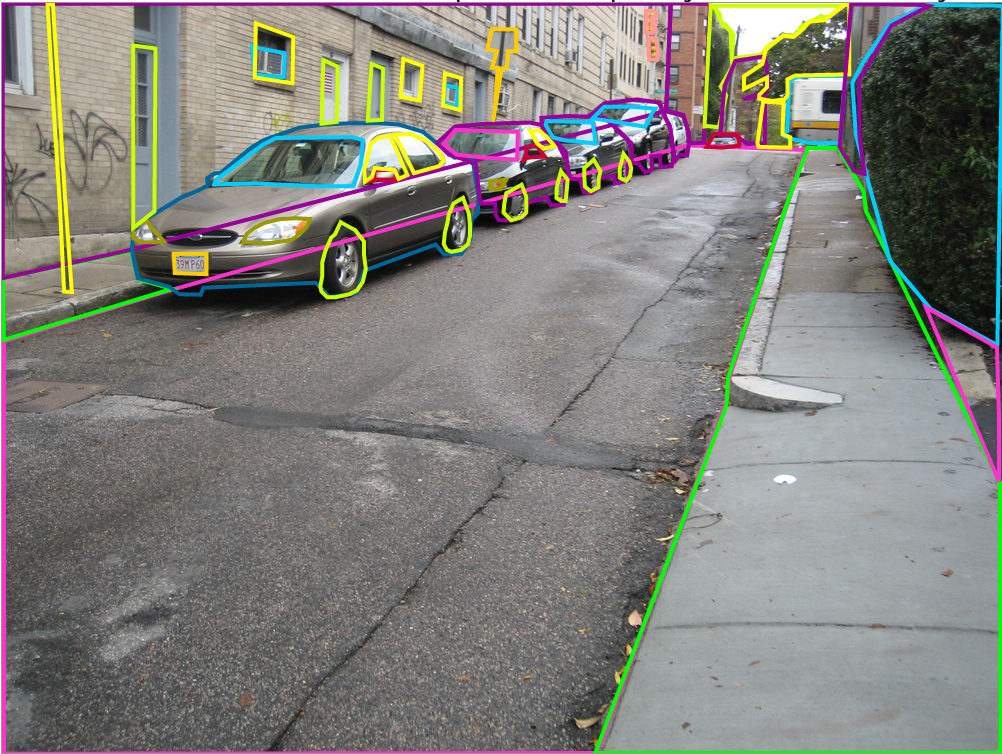
\includegraphics[height=2in]{images/labelmeparse.png}
\caption{An example of a parsed image. Adapted from the website of the
  LabelMe dataset.}
\end{figure*}

 \footnote{cite labelme}

\begin{tabular}{l l}
air conditioning & building\\
bus & car\\
door & headlight\\
license plate & mirror\\
plant & pole\\
road & sidewalk\\
sign & sky\\
traffic light & tree\\
wall & wheel\\
window & windshield\\
\end{tabular}

This is partly motivated by consideration of the human visual system:
\footnote{Pedro suggests Palmer for this whole thing, presumably:

  Palmer, S.E. (1999) Vision Science: Photons to Phenomenology, MIT
  Press .}  
\begin{itemize}
\item Humans use context to resolve ambiguities. \cite{visual-context}
  This means that we can only identify some objects by modeling their
  relationship to other objects. This can be seen in \cite{pop}.
\item Humans interpret some groupings of objects as a larger level
  object or activity, such as crowds of people or flocks of birds.
  Gestalt research demonstrates that perception has definite,
  repeatable grouping rules. \cite{gestalt}
\item Humans seem to interpret whole scenes even when answering
  simpler visual questions, such as edge detection and segmentation.
  This can be seen in Figure \ref{fig-bsd}, which shows an example
  from the Berkeley Segmentation Database. \cite{bsd}
\end{itemize}
\begin{figure}
  \centering
\subfloat[Human Segmentation]{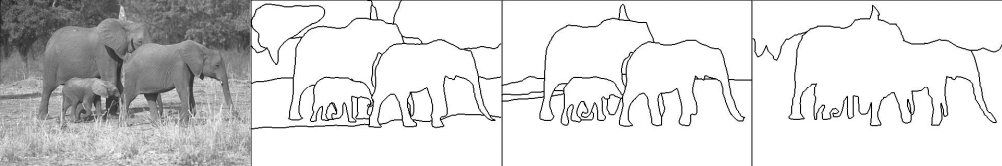
\includegraphics[width=120mm]{images/elephant-human.png}}\\
\subfloat[Machine Segmentation]{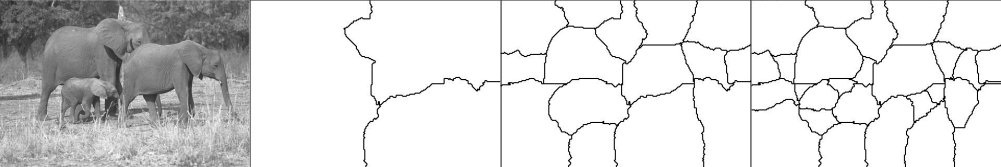
\includegraphics[width=120mm]{images/elephant-machine.png}}
\caption{Even on low-level visual tasks such as segmentation, humans
  give answers based on an interpretation of the whole scene. Figure
  adapted from.}
\label{fig-bsd}
\end{figure}

\footnote{ \cite{bsd}}

Grammatical methods are also motivated by theoretical
considerations. They are a natural choice for modeling large
structural variations (see Section \ref{sec-structural}). Grammatical
models give a principled way to avoid hard decisions for low-level
visual tasks (see Section \ref{sec-soft}). They allow strong models of
background clutter (see Section \ref{sec-clutter}). They allow whole
scene parsing (see Section \ref{sec-whole}). They make it easy to
integrate models from other domains into visual models (see Section
\ref{sec-modules}). Finally, there are theoretical reasons why
grammars may provide better generalization than other models.

\section{Curve Models: An Evolution}

We wish to build probabilistic models of curves, so that we can
calculate a likelihood that a shape class generated a particular
curve. We start by imagining a single input curve, and perturbing it.

The most straightforward model for perturbing a curve is a Markov-type
model. A curve is a sequence of line segments
$\ell_1,\dots,\ell_k$. We can describe the curve by giving the length
$l_i$ of each $\ell_i$, and the angle $\theta_i$ between $\ell_i$ and
$\ell_{i+1}$. If we perturb each $\l_i$ and $\theta_i$ slightly, we
get a curve which differs from the original. Some samples from this
are shown in Figure \ref{fig-markov}.
\begin{figure}
  \centering
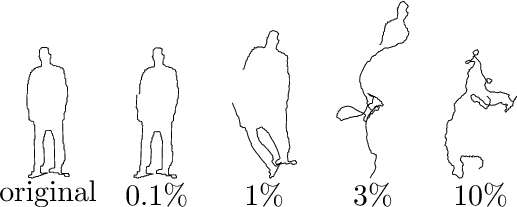
\includegraphics[width=120mm]{images/markov_new.png}
\caption{The problem of drift makes a Markov model unappealing. Random
  samples from this model are too similar locally and too dissimilar
  globally. These shapes were generated by changing each length $l$ by
  a multiplicative factor of $1 + \NNN(0,\sigma)$, and changing each
  angle $\theta$ by adding $\pi \cdot \NNN(0,\sigma )$. Here $\sigma$
  is the value listed underneath the shape.}
\label{fig-markov}
\end{figure}

\begin{figure}
  \centering
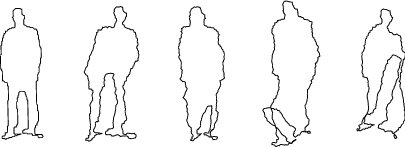
\includegraphics[width=120mm]{images/hcm.png}
\caption{The shape on the left is the original, and the other curves
  have been produced by sampling from the hierarchical curve models of
  . The model produces curves which have more perceptual
  similarity than the Markov model. }
\label{fig-hcm}
\end{figure}
\footnote{\cite{hcm}}

The major weakness of the Markov model is \emph{drift}: the small
errors will accumulate, and the overall shape of the curve will vary
greatly. A straight line has some probability of curling into a tight
spiral. Consider a shape like a hand: a hand has fingers that
protrude. This means that there are two points (namely the two points
where a finger meets the rest of the hand) far away in the curve that
we always expect to be very close together. A Markov perturbation of
the shape is likely to pull these points far apart.

To defeat this problem, \emph{hierarchical curve models} were
introduced in \cite{hcm}. There, the following curve model is given:
\begin{itemize}
\item Given a model curve $C$, decompose $C$ hierarchically by
  repeatedly cutting it in half, in a balanced but otherwise arbitrary
  fashion.
\item Suppose our first decomposition is $C=DE$. We perturb $C$ into
  $C'$ by first perturbing the midpoint of $C$ slightly. We then
  rotate and scale the curves $D$ and $E$ so that $D'$ goes from the
  endpoint of $D$ to the new midpoint, and $E'$ goes from the new
  midpoint to the endpoint of $E$.
\item We then recursively apply the same process to each subcurve $D$
  and $E$. 
\end{itemize}
It is easy to see that this defeats the problem of drift, because the
overall shape of the curve is determined in a constant number of
substitutions from the beginning curve. If our perturbations are
smaller for larger curves, then we will leave the overall shape very
similar while allowing significant local variation. Some samples from
this model are shown in Figure \ref{fig-hcm}.

Hierarchical curve models have room for improvement, as can be seen in
Figure \ref{fig-hcm}. The variations do not respect the perceptual
structure of the original curve; in particular, we do not see
articulated parts being articulated.

In this document, we describe a grammatical reformulation of the work
of \cite{hcm}, which we hope will improve upon it in two
ways. Firstly, we hope to allow for structural variation, which we
argue is an important goal for computer vision in Section
\ref{sec-structural}. Secondly, we give a generative probabilistic model of
curves, which allows us to retrain the parameters of a grammar in a
mathematically sound way, rather than optimizing many parameters in an
expensive and fragile way.

\section{Examples of Grammatical Approaches}

\subsection{Curve Grammars}

We wish to build a model of closed curves in the plane. This is an
important task because curves are the boundaries of objects, and we
can use this fact to recognize some object classes. The shape of a
boundary is invariant to many photometric effects, in particular
illumination. \cite{canny}

\subsection{Visual Chalkboard}

As an example throughout this document, we discuss a system which
would take images of a classroom chalkboard and attempt to parse them
into lecture notes. This is an application with lots of noise. It is
also an application where different levels of interpretation are
required, since lectures can contain both sentences (which should be
interpreted thoroughly, as text) and drawings (which could be
interpreted partially as collections of lines, but which may contain
unsummarizable elements which must be included verbatim).

In Section \ref{sec-modules}, we argue that grammars are a natural
choice for such an application, because they make it possible to
integrate statistical models from other domains in a straightforward
and principled manner.

\subsection{Visual Search Engine}

Google image search is a nice and useful thing, but it relies
partially on images being associated with relevant text on web
pages. It would be nice to find raw or under-described images, and it
would be nice to base search results more on the contents of the
image. We might also submit images as queries, rather than text. The
LabelMe dataset is a good challenge for this task.

In Section \ref{sec-annotation}, we argue that hierarchical
decomposition would allow the necessary rich understanding of
relationships between objects.

\subsection{Other Visual Grammars}
\label{sec-other-grammars}

Many well-performing vision algorithms can be thought of as special
cases of grammatical algorithms. Some examples can be found in
\cite{pop, pictorial, grammar-tr}. Recognizing these as a special case
means that we may be able to improve upon this work by specifying
richer models in some cases, or models that are better mathematically
founded (and thus potentially trainable) in other cases. There are two
tricks for turning a model into a grammar model:
\begin{itemize}
\item Mixture models are a special case of grammar models. If we have
  mixture components $M_1,\dots,M_k$ with mixture weights
  $p_1,\dots,p_k$, then we can build a grammar model $M$ in which we
  have rules:
  \begin{align*}
    M &\to M_1 &(p_1)\\
     &\to M_2 &(p_2)\\
     &\dots&\\
     &\to M_k &(p_k)\\
  \end{align*}
  The same is true of nearest neighbor models. This is exciting
  because mixture models and nearest neighbor models are often very
  powerful, but do not generalize well from a small amount of data.

\item Deformable parts-based models are a special case of grammar
  models. Let $M(x)$ denote the hypothesis that model $M$ appears at
  image location $x$. If we have part models $P_1,\dots,P_k$, then we
  can build a grammar model $M$ which has the rules:
  \begin{align*}
M(x) &\to P_1(x + \delta_1) + \dots + P_k(x + \delta_k)\\
P_i(x) &\to P_i(x+\Delta)\\
P_i(x) &\to I(x_1 \pm w_i, x_2 \pm h_i)
  \end{align*}
  The $\delta_i$ represent the ideal displacement of each part $P_i$
  from the object model. The model is deformable because the second
  kind of rule allows the parts to be randomly displaced. The
  probability of $P_i(x) \to P_i(x+\Delta)$ will depend on
  $\Delta$. The third kind of rule gives the cost to place a part,
  which can be thought of as the negative log probability that a part
  $P_i$ would produce the image data under it, $I(x_1\pm w_i, x_2\pm
  h_i)$.

  In our model of curve grammars, the second kind of rule is given
  by the midpoint distribution $\mu_{X\to YZ}$, and the third kind of
  rule is trivial (see Section \ref{sec-pcfsg}).
\end{itemize}

\section{Grammatical Vision is Important}

\section{Hierarchical Decomposition and Rich Description}
\label{sec-annotation}

It would be very useful if vision algorithms could achieve richer
understanding of scenes, and produce richer descriptions of images. A
rich understanding of a scene requires an understanding of the
relationship between objects. Consider an image containing a person
and two objects, where the person is pointing at one of the
objects. This is an important piece of information, and it cannot
easily be described by a list of the objects in the image.

Some scenes contain important objects that are nothing more than a
particular grouping of other objects: a crowd is just a collection of
people. Moreover, the nature of the collective object is determined
partly by the relationship between its elements. A crowd and a
marching band are two very different objects, but this difference
cannot be expressed in a simple listing of objects. How can vision
algorithms achieve this level of understanding, or even represent it?

One straightforward and general framework for rich description is a
labeled hierarchical decomposition of a
scene. \cite{zhu-mumford} This takes the form of a tree, where:
\bitem
\item The root node describes the entire image.
\item Each node is labeled with the name of an object, and an area of the image described. These areas may be approximate.
\item The children of a node describe sub-parts of the parent, and
  have areas inside the parent node's area.
\eitem
We can explicitly encode such a description in an XML-like language.
Since grammatical methods produce and work with such hierarchical
decompositions, they give a natural model for such structures.

In the example of the visual chalkboard, rich description would
produce more useful output than simple text. For instance, in
transcribing a series of boards as lecture notes, we would like to be
able to label non-textual regions as figures and include them
verbatim, or render them as a collection of lines.

\subsection{Training on rich annotations}

We would also like to train grammars simultaneously on an image and a
hand-made rich hierarchical description of that image. This ensures
that our trained grammars will produce semantically meaningful
decompositions of new images: the decomposition will have a structure
similar to that produced by a human, and we will be able to transfer
labels onto the nodes of the decomposition.

This will make it more feasible to output meaningful rich descriptions
on a wide range of data. Stochastic grammatical methods allow us to
put soft constraints on descriptions (``it is unlikely that a person
will have an apple for a face''), which will be more flexible and less
brittle than hard constraints (``a person's face can have eyes, nose,
etc., but not fruit''). We can thus favor more realistic descriptions
of scenes while still producing useful output on very unrealistic
scenes (such as Magritte's ``The Son of Man'').

Note that we may still gain information from rich descriptions without
a specified correspondence to particular parts of the image. Knowing
the correct structure and guessing at the exact correspondence is no
harder than guessing both the correct structure and the
correspondence. Such descriptions would be less labor-intensive to
produce, so we might be able to train on larger datasets.

In general, supervised learning is easier than unsupervised
learning. In computational linguistics, this means that learning a
grammar for natural language is much more tractable given samples of
natural language that have been parsed. (These are called
\emph{bracketed samples}.) It is likely that training on rich
annotations would also make learning visual grammars much easier.

\subsection{Some Problems with Rich Description, and Solutions}

For a number of reasons, dealing with rich descriptions is more
complicated than dealing with simpler descriptions. Grammatical
methods and hierarchical decomposition give ways around some of these
problems. Some important issues are: Class/Subclass ambiguity
and Questionable Parts.

First, it is worth noting that hierarchical decomposition degrades
gracefully into a flat description, since we can always decompose the
root node into a list of objects. Hierarchical decomposition presses,
but does not force, us to explain how any two parts of our annotation
are related, making for more useful description.

\bitem

\item Decomposition provides a reasonable and elegant solution to the
  Questionable Parts problem. David Marr explained it thus:
  \begin{quote}


    % What, for example, is an object, and what makes it so special that
    % it should be recoverable as a region in an image?

    Is a nose an object? Is a head one?  Is it still one if it is
    attached to a body?  What about a man on horseback?

    These questions show that the difficulties in trying to formulate
    what should be [considered an object] %recovered as a region from
                                %an image 
    are so great as to amount to philosophical problems.  There really
    is no answer to them - all these things can be an object if you
    want to think of them that way, or they can be a part of a larger
    object...% (a fact that is captured quite precisely in Chapter 5).
    \cite{marr}
  \end{quote}

  In any annotation system rich enough that we might simultaneously
  label a wheel and a car, or eyes and a face, in the same image,
  there is an arbitrary choice of how many things to label. Forcing
  these descriptions to be consistent is very
  difficult. \cite{labelme} This is especially pronounced with
  agglomerations, like crowds of people. There is no point at which a
  group of people meaningfully becomes a ``crowd''; two people are not
  considered a crowd, and one hundred people are considered a crowd,
  but it is impossible to draw a clear line between crowds and
  not-crowds.

Forcing consistency may even be counter-productive. If we must label
every face in a crowd, then a crowd seen from a distance will have an
enormous number of face labels, most of which are basically
guesses. If we never label faces in a crowd, then our visual search
engine may fail to retrieve images of a particular person when they
are in a group, even if they are clearly visible. 
  
Hierarchical decomposition describes a scene as a hierarchy of
objects, and further decomposition of these objects is optional; as
long as we know something about the object's appearance, we don't have
to demand that it be broken up into its constituent parts.

\item Grammatical methods also naturally address the Class/Subclass
  Ambiguity problem: descriptions of an object can be general or
  specific, and the level of specificity is fairly arbitrary. It is
  clear that we want the query ``dancer'' in a visual search engine to
  return images of people dancing, but these same images should also
  be returned on the query ``person''. 

  Grammatical methods model such ambiguity as OR nodes in an AND-OR
  structure \cite{zhu-mumford}, or by rules of the form
\begin{align*}
\mathrm{CLASS} &\to \mathrm{SUBCLASS}_1\\
&\to \dots\\
&\to \mathrm{SUBCLASS}_k .\\
\end{align*}

The LabelMe dataset uses a set of labels derived from WordNet
\cite{wordnet} that are related via class-subclass
relationships. The maintainers of the dataset claim that it requires
very little work to map the arbitrary labels provided by users into
these more precise and formalized labels. \cite{labelme} Given
such techniques, the Class-Subclass ambiguity problem is probably not
a fundamental barrier to rich description.

\eitem

\subsection{Rich Description and XML}

The rich descriptions we have described are naturally represented in
XML and similar languages, which yields some opportunities: 

\begin{itemize}
\item XML is reasonably human-readable and human-writable. (Comparable
  formats like YAML are even more so.) This means that rich
  photo-tagging could be done by many people, and also that many users
  could benefit from a visual search engine that accepts structured
  queries. For example, photos inside of an image could be recursively
  described as such, allowing us to separate the images containing an
  actual movie star from those containing a poster depicting that
  movie star. As another example, having a notion of classes and
  subclasses would allow us to search for \texttt{BASS < FISH} and
  receive only pictures of bass fish, and not pictures of the
  instrument or of other fish.

\item Existing technology such as XPath allows computer programs to do
  efficient and flexible searches on XML documents. This means that
  fairly complex image-sorting tasks could potentially be automated.
  This could be very good, because some image-sorting tasks such as
  content moderation are reported to be very psychologically
  damaging when performed by humans.

\item One particular XML-based file format is the \emph{scalable
    vector graphics} format (SVG). If we can learn rich visual
  grammars, we could hope to recover artistic information from images,
  so that we could approximate a drawing as a collection of strokes in
  fills in an SVG document.

  Ultimately, we might hope to learn artistic concepts such as drawing
  style or font, which would greatly expand the power of graphics
  programs.
\end{itemize}

\section{Grammars and Statistical Models}

\subsection{Structural Variation}
\label{sec-structural}

Natural object categories such as cars and people exhibit two kinds of
variation: small deformations and large structural
variation. Therefore, object models which allow for both will make
vision algorithms much more powerful.  The potential for a satisfying
account of large structural variation is one of the most intriguing
possibilities of grammatical methods.

One of the simplest structural variations is occlusion: part of an
object may not be visible, usually because something between the
object and the camera is occluding it. Occlusion has been well
understood in computer vision for a long time, and models can be made
robust to it, e.g., the Hausdorff distance in \cite{hausdorff}. 

Another common way that objects exhibit structural variation is by
having \emph{optional parts}: a dog may or may not have a tail, a
person may or may not have a hat. Occlusion models are capable of
recognizing such objects with or without their optional parts, but
they do not accurately model optional parts. An optional part is a
particular subset of the object that is likely to not appear, while
occlusion allows any not-too-large subset of the model to disappear.

The usefulness of more general structural variation can be seen in
Figure \ref{fig-variation}. Here, the human eye notices a large
similarity between the two shapes $A_1$ and $A_2$, but many curve
models would see very little similarity.

\begin{figure}
  \centering
\subfloat[$A_1$]{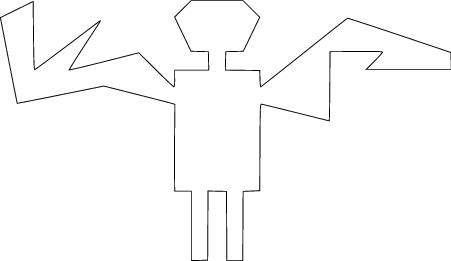
\includegraphics[height=30mm]{images/basri_original.png}}
\subfloat[$A_2$]{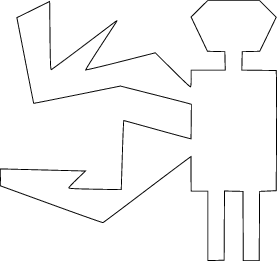
\includegraphics[height=30mm]{images/basri_variation.png}}\\
\subfloat[$A_3$]{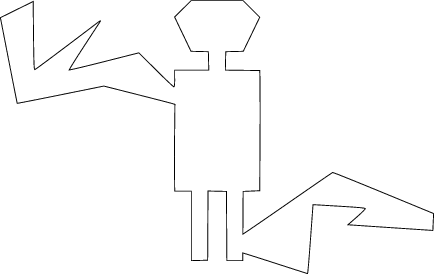
\includegraphics[height=30mm]{images/basri_variation_bad2.png}}
\subfloat[$A_4$]{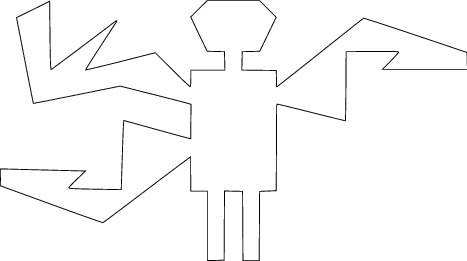
\includegraphics[height=30mm]{images/basri_three.png}}
\caption{If $A_1$ is the original curve, which other curve is most
  similar to it? Figure adapted from .}
\label{fig-variation}
\end{figure}
\footnote{\cite{basri-jacobs}}

We might intuitively describe the second shape, $A_2$, as
$$ A_2 =\mbox{``Take $A_1$, snap off the right appendage, and reattach
  it beneath the left appendage.''}. \label{desc-variation}$$ 
This highlights several important points:

The description \ref{desc-variation} of $A_2$ is very short in
English, and might be even shorter in a specialized curve model
encoding. Description length is a good proxy for the conditional
probability of observing $A_2$ given that it is a distortion of $A_1$
\cite{potter-geman-bienenstock}.

Structural variation is a fundamental problem in modeling visual
objects. In the absence of a practical model of structural variation,
we must model variation as continuous deformation. Then, any model
that declares $A_1$ and $A_2$ to be similar will think that $A_3$ or
$A_4$ is even more similar to $A_1$.

Structural variation cannot be modeled without a semantically
meaningful decomposition of the original curve, like that seen in
Figure \ref{fig-variation-decompose}. Description \ref{desc-variation}
crucially relies on ``the right appendage'' making sense to the
listener. Thus, perceptually simple structural variation must respect
the perceived structure of the original curve. Contrast Figure
\ref{fig-variation} with Figure \ref{fig-badvariation}, where a
similar transformation has been applied with no regard to the
perceived structure of the original curve.

\begin{figure}[h]
\centering
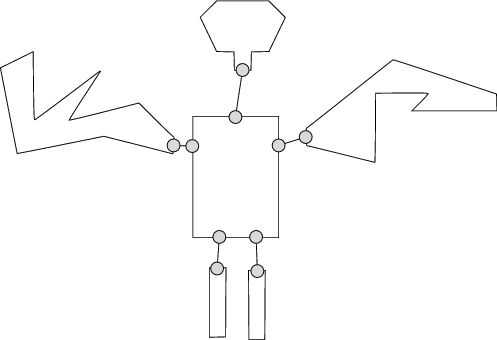
\includegraphics[height=30mm]{images/basri_decomposed.png} 
\caption{The original shape from Figure \ref{fig-variation},
  decomposed into semantically meaningful parts. We argue that this
  decomposition explains why the variation in Figure
  \ref{fig-variation} is less semantically different than the
  variation in Figure \ref{fig-badvariation}. Adapted from
.}
\label{fig-variation-decompose}
\end{figure}
\footnote{\cite{basri-jacobs}}

\begin{figure}[h]
\centering
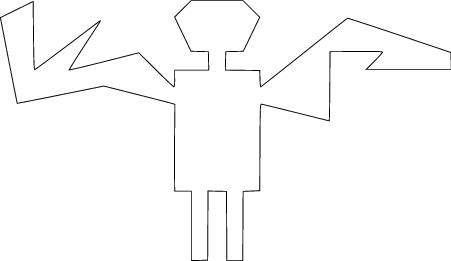
\includegraphics[height=30mm]{images/basri_original.png} 
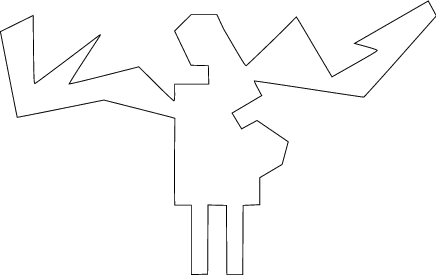
\includegraphics[height=30mm]{images/basri_variation_bad.png} 
\caption{Two shapes which are not perceptually very similar, although
  they are related by a transformation as simple as that in Figure
  \ref{fig-variation}. The problem is that the transformation does not
  respect the perceived structure of the original. Adapted from
  .}
\label{fig-badvariation}
\end{figure}
\footnote{\cite{basri-jacobs}}

Mixture models are a class of models that do not suffer from the
continuous deformation problem of Figure \ref{fig-variation}. However,
if there are multiple independent structural variations possible, it
is unlikely that we will see every combination of each form.  Consider
the shape grammar $\GGG_n$ that generates shapes that have $n$ arms,
each of which can take either of two forms:
\begin{align*}
S&\to \underbrace{Z\dots Z}\\
&\phantom{\to Z ..}n\\
Z &\to A\\
Z &\to B,
\end{align*}
where $A$ is pointy and $B$ is rectangular. We show four shapes
possible under this grammar in Figure \ref{fig-narms}. 
\marginnote{Change these to outline instead of solid shapes!}
\begin{figure}[h]
\centering

\includegraphics[height=30mm]{images/narms.png} 
\caption{Four shapes from $\GGG_8$.}
\label{fig-narms}
\end{figure}
A classic mixture model will not be able to generalize in this
scenario without exponentially many training examples, since there
are $2^n$ possible shapes. If we instead have mixture models at the
level of individual structural variations, then our model is a
grammatical model in the style of Section \ref{sec-other-grammars}.


\subsection{Soft Decisions}
\label{sec-soft}

While human vision crucially relies on global context to resolve local
ambiguity \cite{visual-context}, computer vision algorithms often have
a pipeline which makes hard low-level decisions about image
interpretation, and then uses this output as input to higher-level
analysis. Algorithms will be more accurate and less brittle if they
can avoid making such hard decisions, as advocated in \cite{pop,
  jin-geman}.

For example, in the visual chalkboard, there will be various stray
marks on the chalkboard. We would prefer not to filter these out with
some sort of quality threshold, but instead mark them as
possibilities, try to assemble an overall interpretation of the board,
and then discount any stray marks that do not participate in the
interpretation. This seems much more fruitful than filtering out stray
marks, along with some genuine letters, and then having to be very
forgiving of words actually missing some of their letters altogether.

This requires us to combine and resolve information at different
levels. Grammatical methods provide us with powerful inference
algorithms for determining the most likely decomposition of a scene
under a given compositional model. Since important local ambiguities
will lead to different global decompositions, this is exactly what is
needed: the overall likelihood of the decomposition is a common
currency that allows us to negotiate between fitting the local data
well, and explaining the local data in a way that allows a good
decomposition of the rest of the image.

\subsection{Modeling Clutter with Object Sub-parts}
\label{sec-clutter}

We would like to build specific and accurate models of clutter.  For
instance, for the visual chalkboard, it would be helpful to have a
model for stray chalk marks, rather than a model for arbitrary
unexplained patches; otherwise we will be tempted to explain stray
chalk marks as some letter, possibly a lower-case 'i'. If we try to
set our threshold high enough that we don't do this, we might start
labeling some genuine i's as background. If we instead have a model
for chalk marks, we can explain stray chalk marks and i's as
particular sorts of chalk marks, and differentiate them based on
context and appearance.

\cite{jin-geman} suggests modeling clutter in the background with
sub-parts of the objects of interest. Since objects in the background
are still objects, and are often related to the objects of interest,
this might allow us to build a much stronger background model in many
cases. In addition, by modeling clutter with sub-parts, we are less
likely to hallucinate whole objects when we see sub-parts. Thus, it is
especially important that we have a cheap way to explain clutter that
closely resembles sub-parts of the objects of interest.

With such a system, we might even be able to ignore rather subtle
clutter, such as some stray letters, or even words, from a previous
lecture that was not completely erased. Clutter words would not be
part of a line of text, and would thus be identifiable as clutter in
the parsed output, where they would be excluded from the main body of
text.

\subsection{Whole Scene Parsing}
\label{sec-whole}

It is useful to demand whole scene parses, since it avoids the need to
fine-tune detection thresholds and decision boundaries
\cite{pop}. Consider the example of the visual chalkboard. Instead of
having to set a filter on chalk marks to filter out stray chalk marks,
we simply explain them and discount them, since they are not part of
any larger structure, such as a word, that we find interesting.

\subsection{Statistical Modules}
\label{sec-modules}

Grammatical methods offer a very powerful and general way to make
vision algorithms more robust: if we can integrate different
statistical models in a modular fashion, especially models trained in
different contexts, then our system will be more robust than any
single model.

Grammatical methods are well-suited to integrating any statistical
model that depends on the qualities of image objects and the
relationships between them. When we can map objects and relationships
between domains (for example, mapping pictures of text to actual
text), this allows us to import already-trained statistical models
from very different domains.

Consider transcribing a lecture from the visual chalkboard. The system
will better recover from misidentifying letters if it uses
higher-level knowledge about the lecture's language and contents. In
particular, we can build a single grammar that integrates such
tried-and-true models as the $n$-gram model of letters
\cite{manning-schutze}, the $n$-gram model of words
\cite{manning-schutze}, a stochastic grammar model of phrase and
sentence structure \cite{manning-schutze}, and topic models of word
choice in the subject of the lecture \cite{lda}. All of these models
can be trained on large corpora of text, rather than on smaller
datasets of images.

% Each of these models can easily be expressed in a grammatical way,
% since each gives a likelihood that can be written as a product over a
% decompositional tree structure: 
% \bitem
% \item The $n$-gram models can be written as a product over any tree
%   that respects the linear order of the letters or words. Each factor
%   judges the likelihood of the $n$-grams that bridge the two
%   subtrees.
% \item The stochastic grammar model is itself a grammar, and the
%   trees are the same.
% \item The topic model can simply penalize the nodes corresponding to
%   words according to how common each word is.
% \eitem

% Grammatical methods can potentially express rich relationships between
% model parts through the formation probabilities $\Phi_{M\to P_1\dots
%   P_k}$ considered in Section \ref{sec-other-grammars}.

\subsection{Independence and the Poverty of Stimulus}

Grammatical models are typically context-free, which is fundamentally
about making independence assumptions. We argue that independence
assumptions can increase the effective amount of training data you
have.

\begin{rem}[Context-freeness is an independence assumption]
Grammatical methods in general are characterized by 1) a method for
decomposing novel data in a hierarchical fashion, and 2) an
explanation for each level of the hierarchy in terms of previously
seen data. For example, in a standard CFG, we will have both a parse
tree over a sentence, and a set of labels for the nodes of the parse
tree. If the CFG has been automatically generated (i.e., no human has
assigned semantic meaning to grammar elements), then the set of labels
for the nodes is just a probability distribution derived from all
parts of the training set that have received the same label. 

For generic grammatical methods, we can assume context-freeness by
specifying that the contents of a node N (all nodes below N in the
hierarchy) are independent of the context in which N appears (all
nodes not below N in the hierarchy) given the data stored at N (its
label and any attributes).
\end{rem}

\begin{rem}[Independence assumptions yield more effective data]
  Independence assumptions let you effectively multiply the amount of
  data you have. Consider the following simple problem: try to
  classify 0-1 vectors into two classes given a bunch of labeled
  examples. Consider the two sort of extreme things we can do: if we
  assume that each coordinate of the vector is independent, we get a
  Naive Bayes classifier, where we basically learn what the
  distribution is over a given coordinate for each class. This can be
  done with a small number of training examples.

  The other extreme is assuming that there is total dependence, that
  there is no relation between any two vectors. Then the maximum
  likelihood classifier (Paranoid Bayes?) is given by seeing how many
  times a specific vector showed up in each class, and picking the
  class where it showed up more often. We would have to guess on any
  novel vector.  

  If the independence assumption is valid for the data, then the Naive
  Bayes classifier acts like the Paranoid Bayes classifier trained on
  a data set that is exponentially larger. (Specifically, for each
  class, we generate all possible vectors that can be made by taking
  the first coordinate of a random example from the class, then taking
  the second coordinate from an independently chosen random example
  from the class, etc.)
\end{rem}

Even when the independence assumption does not apply, context-free grammars
are useful. This can be seen in examining the classic nonsense
sentence "Colorless green ideas sleep furiously". The supposed
weakness of context-free grammars, that the context-free assumption is
unrealistic, is actually a strength, because it allows us to parse and
react to very unrealistic data.

% \section{Computational Considerations}

% \subsection{Bidirectional Pipeline}
% \note{ {\bf (write!, sources)}}

% If we avoid hard decisions whenever possible, our algorithms must sift
% through a larger number of intermediate hypotheses. This can be made
% more efficient by doing a form of data-driven parsing that combines
% the strengths of top-down and bottom-up parsing. One example of this
% approach is given in \cite{astar}.

% \subsection{Sharing Object Parts for an Enormous Object Dictionary}
% \label{sec-shared}

% \note{  {\bf (write!)}}

% \note{Not true that it is impractical! Systems exist! Just say it is difficult, I guess. Should we cite the systems?}
% It is currently impractical for vision systems to know about more than
% a certain number of object classes, something like several hundred for
% adequate performance. It would be very useful if we could increase
% this number, so that we have a vision system capable of dealing with
% tens of thousands of object classes.

% This is impractical unless we can devise algorithms which are
% sublinear in the number of known object classes. This, in turn,
% requires that our set of models admits some sort of search
% structure.

% Some work has been done on hashing image patches.
% \note{find}

% By composing a small set of parts which are very distinguishable, we
% will have an exponentially large number of models. Otherwise, the hash
% table just fills up and we have to go through a bunch of false positives.

% \note{ About 30000 entry-level object categories \cite{biederman}}

% \note{Even with a reasonably small set of parts, we still need to be
%   able to search without enumerating models. This could be something
%   like a k-d tree or a hash function. \cite{biederman}}

% For the visual chalkboard, the letters of the alphabet would form a
% small set of parts that combine to produce many objects, potentially
% any word in a very large dictionary.

\section{Grammatical Vision is Difficult}

Little concrete progress has been made with visual grammars. The
general frameworks have few practical results, and people with
practical results don't seem to have a general framework.  \marginnote{This
  statement feels too strong. But something like this has to be said.}

We are also hindered because the closest equivalent to linguistics is
the cognitive science of vision, which is not as well-stocked with
intermediate hypotheses and sanity checks. For example, in
linguistics, utterances can be decomposed into phonemes. There is no
agreement as to how a visual signal can be decomposed.

\section{Grammar induction is difficult}
\label{sec-gram-hard}

Grammatical methods in vision are inspired by grammatical models like
probabilistic context-free grammars in linguistics. In computation
linguistics, the problem of learning a grammar from unlabeled examples
(grammar induction) is very difficult.

There are many \cite{lee-induction} negative theoretical results, the
most fundamental of them being Gold's Theorem:

\begin{thm}[Gold's Theorem]
Consider an algorithm $A$ trying to learn a language $L\in \Sigma^*$.
$A$ is given an infinite sequence of words $w_1, w_2, \dots\in L$ which
contains every word in $L$ at least once. After each $w_i$, $A$
outputs some $L_i$. $A$ is said to {\em learn $L$ in the limit} if,
for some $n$, $L = L_n = L_{n+1} = L_{n+2} = \dots$.

Then, if a class of languages $\LLL$ contains all languages of
finitely many strings, and at least one infinite language (in
particular, if $\LLL$ is the set of context-free languages), no
algorithm can learn all languages in $\LLL$ in the limit.
\end{thm}
Note that this result applies to all algorithms, regardless of their
complexity. 

This is a fundamental theoretical barrier to grammar induction. There
is some hope that we can defeat it by adopting a Bayesian approach,
and only hoping to learn sufficiently simple grammars. This has been
attempted several times, but no solution is known for the associated
Bayesian learning problem, and a heuristic search strategy must be
used \cite{cook, stolcke, nevill-manning}.

It is clear that the problem of learning context-free grammars applies
directly to curve grammars, since part of our curve model actually is
a PCFG (see Section \ref{sec-pcfsg}). The learning problem might be
easier if visual grammars can be simpler in structure than string
grammars for natural languages. We don't know if this is the case.

\section{Visual Grammars are hard for additional reasons}

\subsection{Comparisons are Always Inexact}

The continuous nature of visual signals means that we will rarely if
ever see exact agreement between two visual objects at the pixel
level. Compare a well-defined linguistic object (such as a word) to a
visual part such as an eye; an eye will look slightly different in
every image because of natural variation and photometric
effects. Because language has predefined symbols, in the case of
written language, or agreed-upon phonemes, in the case of spoken
language, methods from computational linguistics can check whether two
letters or two words are the same. Working with visual grammars is
thus analogous to trying to solve the problems of computational
linguistics simultaneously with the problems of speech recognition.

Computational linguistics algorithms can also be given hand-labeled
information about pre-existing correspondences between samples. For
example, there are datasets of sentences which come with ground-truth
grammatical parses. Such information is generally unavailable in
vision. 

Without certain knowledge of correspondence between samples,
generalization is difficult. We are required to infer correspondences
between samples in an unsupervised manner. This generally leads to a
unsupervised learning problem, such as clustering, or a correspondence
problem.

\subsection{Dealing with Scale}

Computer vision usually tries to be scale invariant, since a small
object closer to the camera naturally looks like a large object
further from the camera. A doubled copy of an image is hopefully
semantically the same as the original image.

We thus have two problems: when an object is too small, its internal
structure may be lost. Generally, fine internal structural elements
first become texture (discernible en masse but not individually) and
then disappear completely. The larger object may still, however, be
recognizable by shape.

When an object is too large, we are faced with the task of parsing
internal structure of which we were previously unaware.

These difficulties can probably be dealt with. The first demands that
we come up with a simple appearance model for every object, so that we
can detect it without detecting any of its subparts. Decreased recall
is probably OK, as smaller things are actually more difficult to see.

The second demands that every object be detectable at large scales,
even those which have no sub-parts in our grammar. We can model this
with simple infinitely recursive grammars; sufficiently simple ones
can hopefully model almost anything, while basically preventing their
being bias for either one of: 
\bitem
\item A ``larger'' model with more internal structure
\item A ``smaller'' model with less internal structure
\eitem

\subsection{Plane grammars do not naturally admit efficient parsing}

Efficient algorithms for parsing strings with context-free grammars
rely on dynamic programming, and ultimately on the fact that a string
has only quadratically many contiguous substrings. The elements of
visual grammars naturally live in the image plane, and thus do not
have a linear order. A visual object need not even occupy a single
contiguous region, in the case of occlusion. Therefore, a parsing
algorithm might in principle have to consider any subset of the image
elements as a node in the parse, leading to an exponential runtime.

There are some ways to address this problem.

% \section{Prior Work and Literature Review }
% \note{{\bf (write!)}}

% \bitem
% \item Visual Grammars:
% \bitem
% \item Stu Geman and Ya Jin's work
% \item visual L-systems
% \eitem
% \item Grammar Induction:
% \bitem
% \item \cite{stolcke}
% \item Dan Klein 
% \item \cite{charniak}
% \eitem
% \eitem

\marginnote{beginning of intro.tex}


\chapter{Grammatical Models of Shape}

  \section{Introduction}
    \marginnote{beginning of models/models\_intro.tex}
Introduction!
\marginnote{end of models/models\_intro.tex}
  

  \section{Goals}
    % models/models_goals.tex

\marginnote{beginning of models/models\_goals.tex}

\begin{itemize}

\item Compare shape grammars to other point-set models
\marginnote{Change ``point-set'' to something else.}

We are building probabilistic models of shape. We want to demonstrate
that our models have nice properties. In particular, we would like to
prove that our models do as well or better in explaining geometric
variability, compared to other popular models of shape. For now, we
consider only models of shape that deal with the location in the plane
of a fixed number of corresponding landmarks, $z_1, \dots, z_n$.

The easiest way to compare two generative probabilistic models is to
examine samples from them, and subjectively assess their similarity to
real data. This is inherently a very qualitative evaluation.

When the other models are also probabilistic models, we can compare
them in a more quantitative way using (estimated) cross-entropy, which
is defined as
$$H(\{x_1,\dots,x_n\}, q) = - \sum_{i=1}^n \frac{1}{N} \log_2 q(x_i).$$

If $X = \{x_1,\dots,x_n\}$ is unseen data, and a large enough sample
to be statistically useful, then $H(X,q)$ is a good measure of how
well a model explains unseen data. Smaller values of $H(X,q)$ suggest
that $q$ is a better model. One problematic aspect of cross-entropy is
that it is only meaningful if $q$ is a correctly normalized
probability distribution. Often it is easier to compute
$\widetilde{q}(x) = Z\cdot q(x)$ for some unknown but fixed constant
$Z$.

When we are comparing to a non-probabilistic model, sampling is
impossible, and cross-entropy is meaningless. In this case, the most
straightforward way to compare models is by using them both in some
task like classification. For instance, we can use both models to
classify leaves as being either oak or maple leaves. Whichever model
has a lower error rate is better capturing the differences between the
two classes of shapes.

We would like to consider the following models:

  - Markov curve models, where we represent a curve as a series of
    turns and line segments (a la the Logo turtle), and then add noise
    to the angle of each turn, and the length of each line segment.
  - Procrustes-type models, such as the Watson distribution and the
    Bingham distribution
  - Independent gaussian perturbations of each point
  - Independent nonparametric perturbations of each point

For our models, we would like to consider several different models:
  - a hand-built model
  - a model automatically inferred from a single example
  - a model automatically inferred from a single example and tuned
    with multiple examples

\item Model curves of varying length

We would like to demonstrate that shape grammars effectively model
curves with varying numbers of points. This is important to achieve
scale invariance, since larger objects will generally have more
detailed boundaries.

For this question, there are fewer standard probabilistic models to
compare grammars to. There are many discriminative models that deal
with curves of varying length. Unfortunately, there are few
classification tasks hard enough to distinguish between different
models. There are more classification tasks when we consider the more
restricted problem of comparing two different shapes, rather than
modeling an entire class and classifying a single shape.

We can examine samples from variable-length grammar models, and we can
try to perform well on classification tasks.

One hard matching task is MPEG-7. We are only allowed to compare
images in pairs, and there are about 2 million pairs that must be
iterated over. Therefore, we must be able to build a grammar from a
single example that is very small and very robust. We must also be
able to make coarse versions of curves that are good stand-ins, since
we will have to lessen the work required to parse. We can start with a
much smaller subset of the dataset, of course.

\item Build more interesting grammars

We would like to demonstrate the expressiveness of grammatical curve
models. In particular, we would like to show that a hand-built grammar
can exhibit interesting variation, such as:
\begin{itemize}      
 \item articulating parts of an object
 \item the presence or absence of a part
 \item a choice between two different variations on the part
 \item shared parts that occur in different contexts 
\end{itemize}

We will show samples from these models.

We also want to do this with automatically inferred grammars, but that
is a hard problem. Section 6 will document our efforts there.

\item Curve Classification

We want to build a system that can classify curves. We will give it a
set of curves from $n$ different classes $C_1,\dots,C_n$, and we wish
to assign new curves to the class that they most belong in. Some
datasets for this task are:
\begin{itemize}
\item Swedish Leaf dataset. Here we are given the silhouettes of
  leaves from fifteen different species of tree. (Species include
  maple, oak, and some sort of willow.) For each class, we are given
  25 example leaves, and then we want to build a classifier that will
  accurately classify another 50 examples from each species.

\item MPEG7.

\item The LabelMe dataset \cite{labelme} has some adequate user-drawn
  polygons for many classes of natural shapes.

\end{itemize}

Our generic approach to this task will be to build a probabilistic
model for each class. Given a novel curve $x_*$ from class $c_*$, we
will compute $\PP( x_* \mid c_* = C_i)$ for each class and assign
$x_*$ to the class which gives it the highest likelihood.

\item Parsing goals

Given a grammar model and a curve, we want to calculate how likely the
curve is under the model, and we would like to extract the most likely
correspondence between the points of the curve and the parts of the
model. We demonstrate parsing with several different tasks:

\begin{itemize}
  \item Given two curves whose points can be put into a one-to-one
    correspondence, show that we can recover that correspondence by
    building a grammar model from one curve and using it to parse the
    other. We can do this either with a hand-built model or an
    automatically generated model.
  \item Given a coarse curve and a finer curve, show that we can recover a
    reasonable correspondence between the points of the coarse curve
    and a subset of the points of the finer curve. We do this by
    building a grammar model from the coarse curve and using it to
    parse the finer curve. This demonstrates that we can model longer
    curves than were used to build the grammar. 
  \item Given a coarse curve and a finer curve, recover a reasonable
    correspondence by building a grammar from the finer curve and
    parsing the coarse curve. This demonstrates that we can model
    shorter curves than were used to build the grammar.
  \item Given a coarse curve and a finer curve, where the finer curve has
    features not present in the coarse curve (such as bumps or pits),
    recover a reasonable correspondence by building a grammar from the
    coarse curve and using it to parse the finer curve. This
    demonstrates that we can model longer curves that have non-trivial
    variation in detail.
  \item Given two fine curves which do not have a perfect correspondence,
    recover a reasonable correspondence by building a grammar from one
    and using it to parse the other. This demonstrates that we can
    model both extra and missing points.
  \item Given a rich grammar, show that we can choose the correct
    structure for input curves.
\end{itemize}

\end{itemize}

\marginnote{end of models/models\_goals.tex}


  \section{Prior Work}

  \section{Motivating Example: L-Systems}
    % lsystems.tex

\marginnote{beginning of models/lsystems.tex}

To motivate our discussion of curve grammars, we will first give an
amusing example of such a grammar, which is inspired by L-systems. A
Lindenmayer system, or L-system, is a parallel string rewriting
system. 
\marginnote{They are intended to be pictures! Cite Lindenmayer's famous book.}
Although they are defined on strings, it is popular to render
their output as a picture using a ``turtle language'' akin to
Logo. They are a simple and intuitive way to generate fractal
images. Since our formalisms do not match up perfectly with the usual
definition of L-systems, we will not discuss them.

We will informally discuss curve rewriting systems, where we
iteratively replace straight lines with curves composed of straight
lines. We will represent our curves like this: \spk{10}{gline}, so that
we remember which endpoint is which.

Consider the following system\footnote{generated by $A=A+A+A--$ with
  angle $60^\circ$ in Inkscape}:
$$ \spk{10}{gline} \to \spk{10}{gbump} .$$

Applying this rule a few times, we generate \spk{10}{gline}, \spk{10}{gbump},
\spk{10}{gbump2} and \spk{15}{gbump3}.

%% An L-system might represent
%% this rewrite rule as $A\to A+A+A$. Here, if we interpret the symbol
%% $A$ as ``go forward one step'' and the symbol $+$ as ``rotate 60
%% degrees to the left'', then a turtle following the directions $A+A+A$
%% would generate the curve 
\includegraphics[width=10mm]{bump.png},
%% suitably rotated.

We now wish to construct a more complicated system. We need to start
distinguishing different kinds of curves, in this case \spk{10}{gdash}
versus \spk{10}{gline}. Consider the following system\footnote{generated by 
$A=B+A+B; B=A-B-A$ with angle $60^\circ$ in Inkscape}
\begin{align*}
\spk{15}{gline} &\to \spk{15}{gBAB} \\
\spk{15}{gdash} &\to \spk{15}{gABA}.
\end{align*}

\marginnote{We should put the things on a commons scale.}
If we start from \spk{10}{gline}, we successively generate
\spk{10}{gBAB}, \spk{20}{gsier2}, and \spk{20}{gsier3}.  Suprisingly,
after a large number of iterations, a pattern arises that may be
familiar: Sierpinski's triangle! After eight iterations, we have
(filling in the dashed lines for simplicity) curve $C$:

\spk{100}{gsier8}.

These curves were generated by Inkscape's L-system function, which has
a randomizing option. It is interesting to randomize the last
example. Here is the randomized version $C'$ I got, with fairly little
noise (10\% randomization in the length of line segments, and 5\%
randomization in the angles. These parameters only make sense in a
more standard L-system framework):

\spk{100}{gbadsier}.


\footnote{This is exactly the issue shape-tree addresses in contrast
  to other deformable models.}  This has no global similarity at all
to the other curve! Inkscape is using a Markov-like source of
randomness, and little errors at the local level add up to huge
changes at the global level. If we are going to have a statistical
model for perceptual similarity of curves, we will have to find a way
to introduce long-range dependencies. This brings us to our next
section: probabilistic context-free grammars on curves.

\marginnote{end of models/lsystems.tex}


  \section{Motivating Example: A Simple Hand-built grammar}
    
\subsection{A hand-built grammar}

Here we are drawing a grammar. We have built this grammar by hand, by
taking the following curve, and specifying a decomposition of it:

\includegraphics[width=2in]{./1.grammars/hand_built/hand_built_curve.eps}

Here is the grammar:

Here are some samples from the grammar:

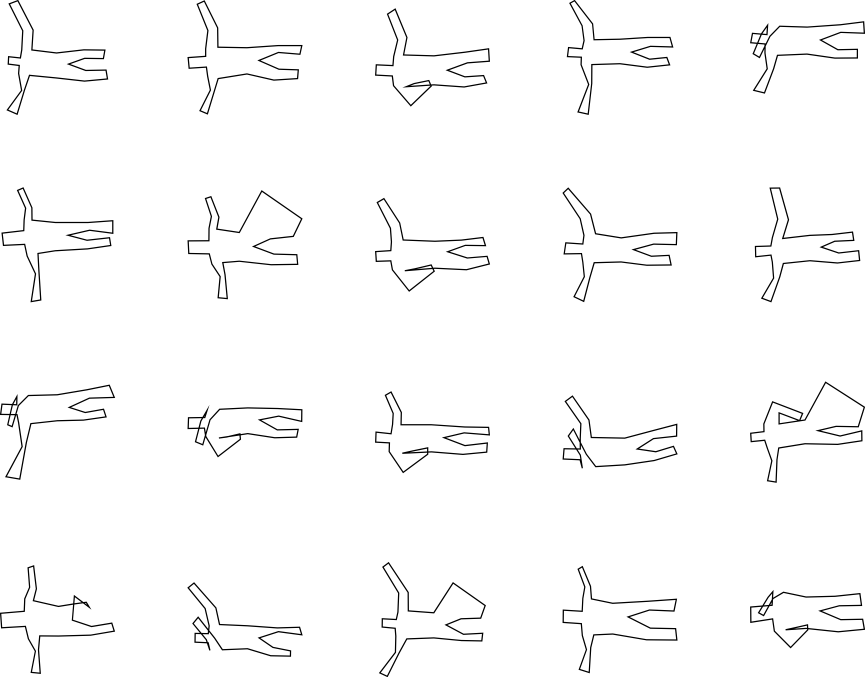
\includegraphics[width=6in]{output/3.learning/incremental/gram.19.d/samples.png}



  \section{Dealing with Curves}
    % curves.tex

A continuous plane curve is a continuous function $C:[0,1]\to
\RR^2$. $C$ is closed if $C(0) = C(1)$. In order to handle curves
computationally, we approximate them with discrete curves (referred to
as ``curves'' hereafter). We create a curve by choosing a finite
number of sample points $p_0,\dots,p_n\in \RR^2$, where $p_i =
C(t_i)$ for some $0\le t_0 < t_1 < \ldots < t_n \le 1$. A curve is
closed if $p_0 = p_n$.

We can concatenate open curves $C$ and $D$ if the last point of $C$ is
the first point of $D$. We will denote this curve by $CD$. 

We will denote an oriented line segment going from point $p$ to point
$q$ by $\ell_{p,q}$. A curve will then have the form
$$ \ell_{p_0,p_1} \ell_{p_1,p_2}\cdots \ell_{p_{n-1},p_n},$$ and
$p_0$ will be equal to $p_n$ iff the curve is closed. For a closed
curve, this sequence is circular, and we consider any cyclic
permutation of the line segments to be the same curve.

We will denote the length of a curve in segments by $|C|$. A curve $C$
will have $|C|+1$ sample points (counting $p_0 = p_n$ doubly if $C$ is
closed). We will denote the $i$-th sample point of $C$ by $C[i]$,
where $i$ ranges from $0$ to $|C|$.


\subsection{Discretizing for Efficiency}

Our inference and learning algorithms run in time that depends on the
number of sample points in a curve. In particular, parsing takes time
that is cubic in the number of sample points. We can therefore vastly
speed up inference and learning by working with subsampled curves. In
this section, we describe an algorithm that approximates the shape of
a curve with another, coarser curve. 

Let $C$ be a curve with $N$ points. We wish to produce a curve $C'$
such that (a) $C'$ approximates the shape of $C$, (b) $|C'| \approx
L$, and (c) $C'$ is sampled relatively uniformly from $C$. We do this
by minimizing the objective function \eqref{eq:subsample-obj}. The first
term measures the total deviation between $C$ and $C'$, and the second
term rewards relatively uniform sampling at the correct rate.
\begin{equation}
\argmin_{ \{n_i \} } \sum_i \sum_{j=0}^{\lambda_i} \left\| p_{n_i+j} -
  \left( \frac{\lambda_i - j}{\lambda_i} p_{n_i} + \frac{j}{\lambda_i}
    p_{n_{i+1}} \right) \right\|^2 + \alpha \sum_i (\lambda_i -
\widehat{\lambda})^2,\label{eq:subsample-obj}
\end{equation}
where $\lambda_i$ is the length of the $i$-th segment and
$\widehat{\lambda} = N/L$ is the ``ideal'' segment length. If $C$ is
closed, then $p_{n_i + j}$ wraps around: $p_{n_i + j} = p_{n_i+j \mod
  N}$ . This minimization can be done with a straightforward dynamic
program. The results of the algorithm can be seen in Figure
\ref{fig-subsample}. Note that, while we lose fine detail, the
resulting curves closely approximate the original curves.
\begin{figure}[h]
\centering
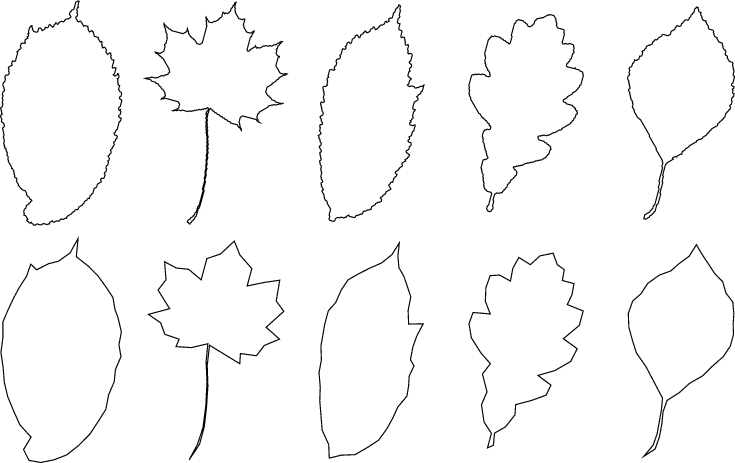
\includegraphics[width=120mm]{images/subsample.png} 
\caption{Subsampled curves. Here $\widehat{\lambda} = 40$}
\label{fig-subsample}
\end{figure}



  \section{Stochastic Shape Grammars: A Generative Model for Curves}
    % curvegrammars.tex: explaining model of curve grammars

\marginnote{beginning of models/curvegrammars.tex}

In this section, we define Probabilistic Context-Free Shape Grammars,
a probabilistic model that allows us to generate random curves, parse
curves to find their likelihood, and ultimately learn distributions
over a class of curves.

Analogously to nonterminals in a traditional context-free grammar, we
introduce {\em placed symbols}. A placed symbol is of the form
$X_{p,q}$, where $X$ is a member of a finite alphabet $\NNN$ or the
special symbol $\ell$, and $p,q$ are points. $X_{p,q}$ represents an
oriented curve going from $p$ to $q$. The path between the endpoints
is unspecified.

\marginnote{Recall \spk{10}{gdash} and \spk{10}{gline} from the
  section on L-systems, which represented different kinds of curves
  because they were on the left-hand side of different productions.}
We specify the type $X$ so that different nonterminals can be related
by the grammar. Therefore, $X$ should be thought of as specifying a
particular class of paths between any two endpoints. By itself, $X$ is
an {\em abstract symbol} that can be instantiated as a placed symbol
between any $p$ and $q$.

The special symbol $\ell$ denotes a line segment. This takes the place
of terminals in traditional context-free grammars.

\begin{defn}
A {\em placed curvilinear form} (by analogy with a sentential form) is
a sequence of placed symbols
$$ \alpha^{(0)}_{p_0,p_1} \alpha^{(1)}_{p_1,p_2} \cdots
\alpha^{(n-1)}_{p_{n-1},{p_n}},$$ where $\alpha \in \NNN \cup \{\ell
\}$.  As with curves, $p_0$ will be equal to $p_n$ iff the curvilinear
form is closed, and two closed curvilinear forms will be considered
equivalent if they differ by a cyclic permutation.

An {\em abstract curvilinear forms} is a sequence of abstract symbols
(with no associated geometric information)
$$ \alpha^{(0)} \alpha^{(1)} \cdots \alpha^{(n-1)}.$$ We will specify
whether these are open or closed, since there is no other way to
tell. Again, closed abstract curvilinear forms will be considered
equivalent if they differ by a cyclic permutation.
\end{defn}

We next introduce substitutions and substitution rules, which allow us
to transform curvilinear forms, ultimately producing curves. We will
perform substitutions of the form
$$ X_{p,q} \to Y^{(1)}_{p,p_1} Y^{(2)}_{p_2,p_3} \cdots
Y^{(k)}_{p_{k-1},q}.$$ Since $X_{p,q}$ represents an unspecified path
from $p$ to $q$, substitution simply gives a more specific route, in
terms of which points we will visit in between (the $p_i$, which we
will call the midpoint if there is only one of them, and {\em control
  points} otherwise) and what sort of path we will follow between
these points (the $Y^{(i)}$).

In order to give a substitution rule for performing substitutions, we
need to give
\bitem
\item An {\em abstract substitution rule} $X\to Y^{(1)}\cdots Y^{(k)}$.
\item a rule for determining the $p_i$ in terms of $p$ and $q$.
\eitem

In practice, applying a substitution rule is problematic because the
$p_i$ live in an infinite domain ($\RR^2$), but we want to deal with
curves that (1) live in a finite domain (the pixels of the image
plane) and (2) are expected to exhibit a good deal of variation. Thus,
we give a distribution $\mu_{X\to Y^{(1)}\cdots Y^{(k)}}(p_1,\dots,
p_{k-1} ; p,q)$ over the $p_i$ called the {\em control point distribution}. 
When there is only a single control point, we will call $\mu_{X\to
YZ}(p_1; p,q)$ the {\em midpoint distribution}.

\begin{defn}
A probabilistic context-free shape grammar (PCFSG) is a tuple 
$\GGG = (\NNN, \RRR, \SSS, \ell, \MMM, \XXX)$, where
\bitem
\item $\NNN$ is a set of abstract symbol types, which we will call
  {\em nonterminals}
\item $\RRR$ is a set of abstract substitution rules, with $\RRR(X)$
  being the set of rules in $\RRR$ with $X$ on the left-hand side
\item $\SSS$ is the {\em starting set} of abstract curvilinear forms
\item $\ell$ is a special curve type representing a line segment
\item $\XXX = \{ \rho_X \mid X\in \NNN \} \cup
  \{\rho_\SSS\}$, where $\rho_X$ is a probability distribution over
  $\RRR(X)$, and $\rho_\SSS$ is a distribution over $\SSS$
\item $\MMM = \{ \mu_{X\to Y^{(1)}\cdots Y^{(k)}} \mid (X\to
  Y^{(1)}\cdots Y^{(k)}) \in \RRR\}$ is a set of control-point
  distributions.
\eitem
\end{defn}

It is worth noting that $\GGG$ has a corresponding {\em abstract
  grammar} $\GGG_{abs} = (\NNN, \RRR, \SSS, \{\ell\}, \XXX)$ which is
just a traditional PCFG. $\GGG_{abs}$ is an odd PCFG because it only
generates strings of the symbol $\ell$; nevertheless, many properties
of $\GGG$ are actually properties of $\GGG_{abs}$.

For a grammar that generates open curves, we can assume that $\SSS$
has a single curvilinear form $S$, and we will call $S$ the start
symbol. We sample from such a PCFSG by starting with the curvilinear
form $S_{p,q}$ for arbitrary $p$ and $q$. While our curvilinear form
contains a placed symbol $X_{p',q'}$ such that $X\ne \ell$, we pick a
random substitution rule $X \to Y^{(1)} \dots Y^{(k)}$ according to
$\rho_X$, and pick random control points $p_1,\dots, p_{k-1}$
according to $\mu_{X\to Y^{(1)}\dots Y^{(k)}}(p_1, \dots, p_{k-1}; p',
q')$. We then replace the placed symbol $X_{p',q'}$ with the
curvilinear form $Y_{p',p_1}^{(1)} \dots Y_{p_{k-1},q'}^{(k)}$. We
will disallow substitutions in which any two control points $p_i, p_j$
are equal, or in which any control point $p_i$ is equal to either of
the endpoints $p'$ or $q'$.

\marginnote{Explain this better}
There is a slight difficulty here in that we usually cannot define the
control-point distribution if $p$ and $q$ are equal. This is
important, since we are mainly interested in closed curves, so we
would like to start with $S_{p,p}$ for some arbitrary $p$. In this
case, our set $\SSS$ of starting forms will contain abstract
curvilinear forms of length two or more, which are understood to be
closed. We choose a random such curvilinear form according to
$\rho_\SSS$, and then continue as before.

\subsection{Restricted Classes of Shape Grammars}

In this section, we define some restricted classes of PCFSG's. Our
restrictions are only on the abstract part of the grammar, so we are
just specifying restricted classes of traditional grammars.

For simplicity and efficiency, we will usually restrict our abstract
grammars to be in Chomsky Normal Form, in which abstract substitution
rules can only be of two forms: 
\bitem
\item Binary rules of the form $X \to Y Z$.
\item Lexical rules of the form $X \to \ell$.
\eitem 

From now on, we will assume that PCFSG's are in Chomsky Normal Form.
Accordingly, we will speak of midpoints, rather than control
points. It is important to note that PCFSG's differ from standard
PCFG's in that not all PCFSG's are equivalent to a PCFSG in Chomsky
Normal Form. This is because not all control point distributions can
be realized as a product of midpoint distributions. For instance,
suppose we have a rule $A\to BCD$, which in the PCFG setting could be
replaced with rules $A\to BX, X\to CD$. We could have a control point
distribution $\mu_{A\to BCD}(p_1,p_2;p,q)$ in which $p_1,p_2$ were on
a random circle going through $p$ and $q$. If we try to replicate such
a control point distribution with midpoint distributions $\mu_{A\to
  BX}(p_1; p,q), \mu_{X\to CD}(p_2; p_1, q)$, we cannot, because the
distribution $\mu_{X\to CD}(p_2; p_1,q)$ can only depend on the two
points $p_1$ and $q$, and that is not sufficient to specify a unique
circle.

\marginnote{end of models/curvegrammars.tex}


    \marginnote{Add a short section on inference. Explain that the
      details of parsing are deferred to the learning section.}
    

\subsection{One-to-one}

Here we have two curves given by hand-annotation of the Romer
dataset. We build a grammar from the curve on the left, using a
hand-built set of constituents. We then parse the curve on the right,
and show the Viterbi parse by showing the correspondences between the
two curves.

Because there are no missing or extra points, this is straightforward.

%% we can use \input{} here to incorporate dynamically generated text

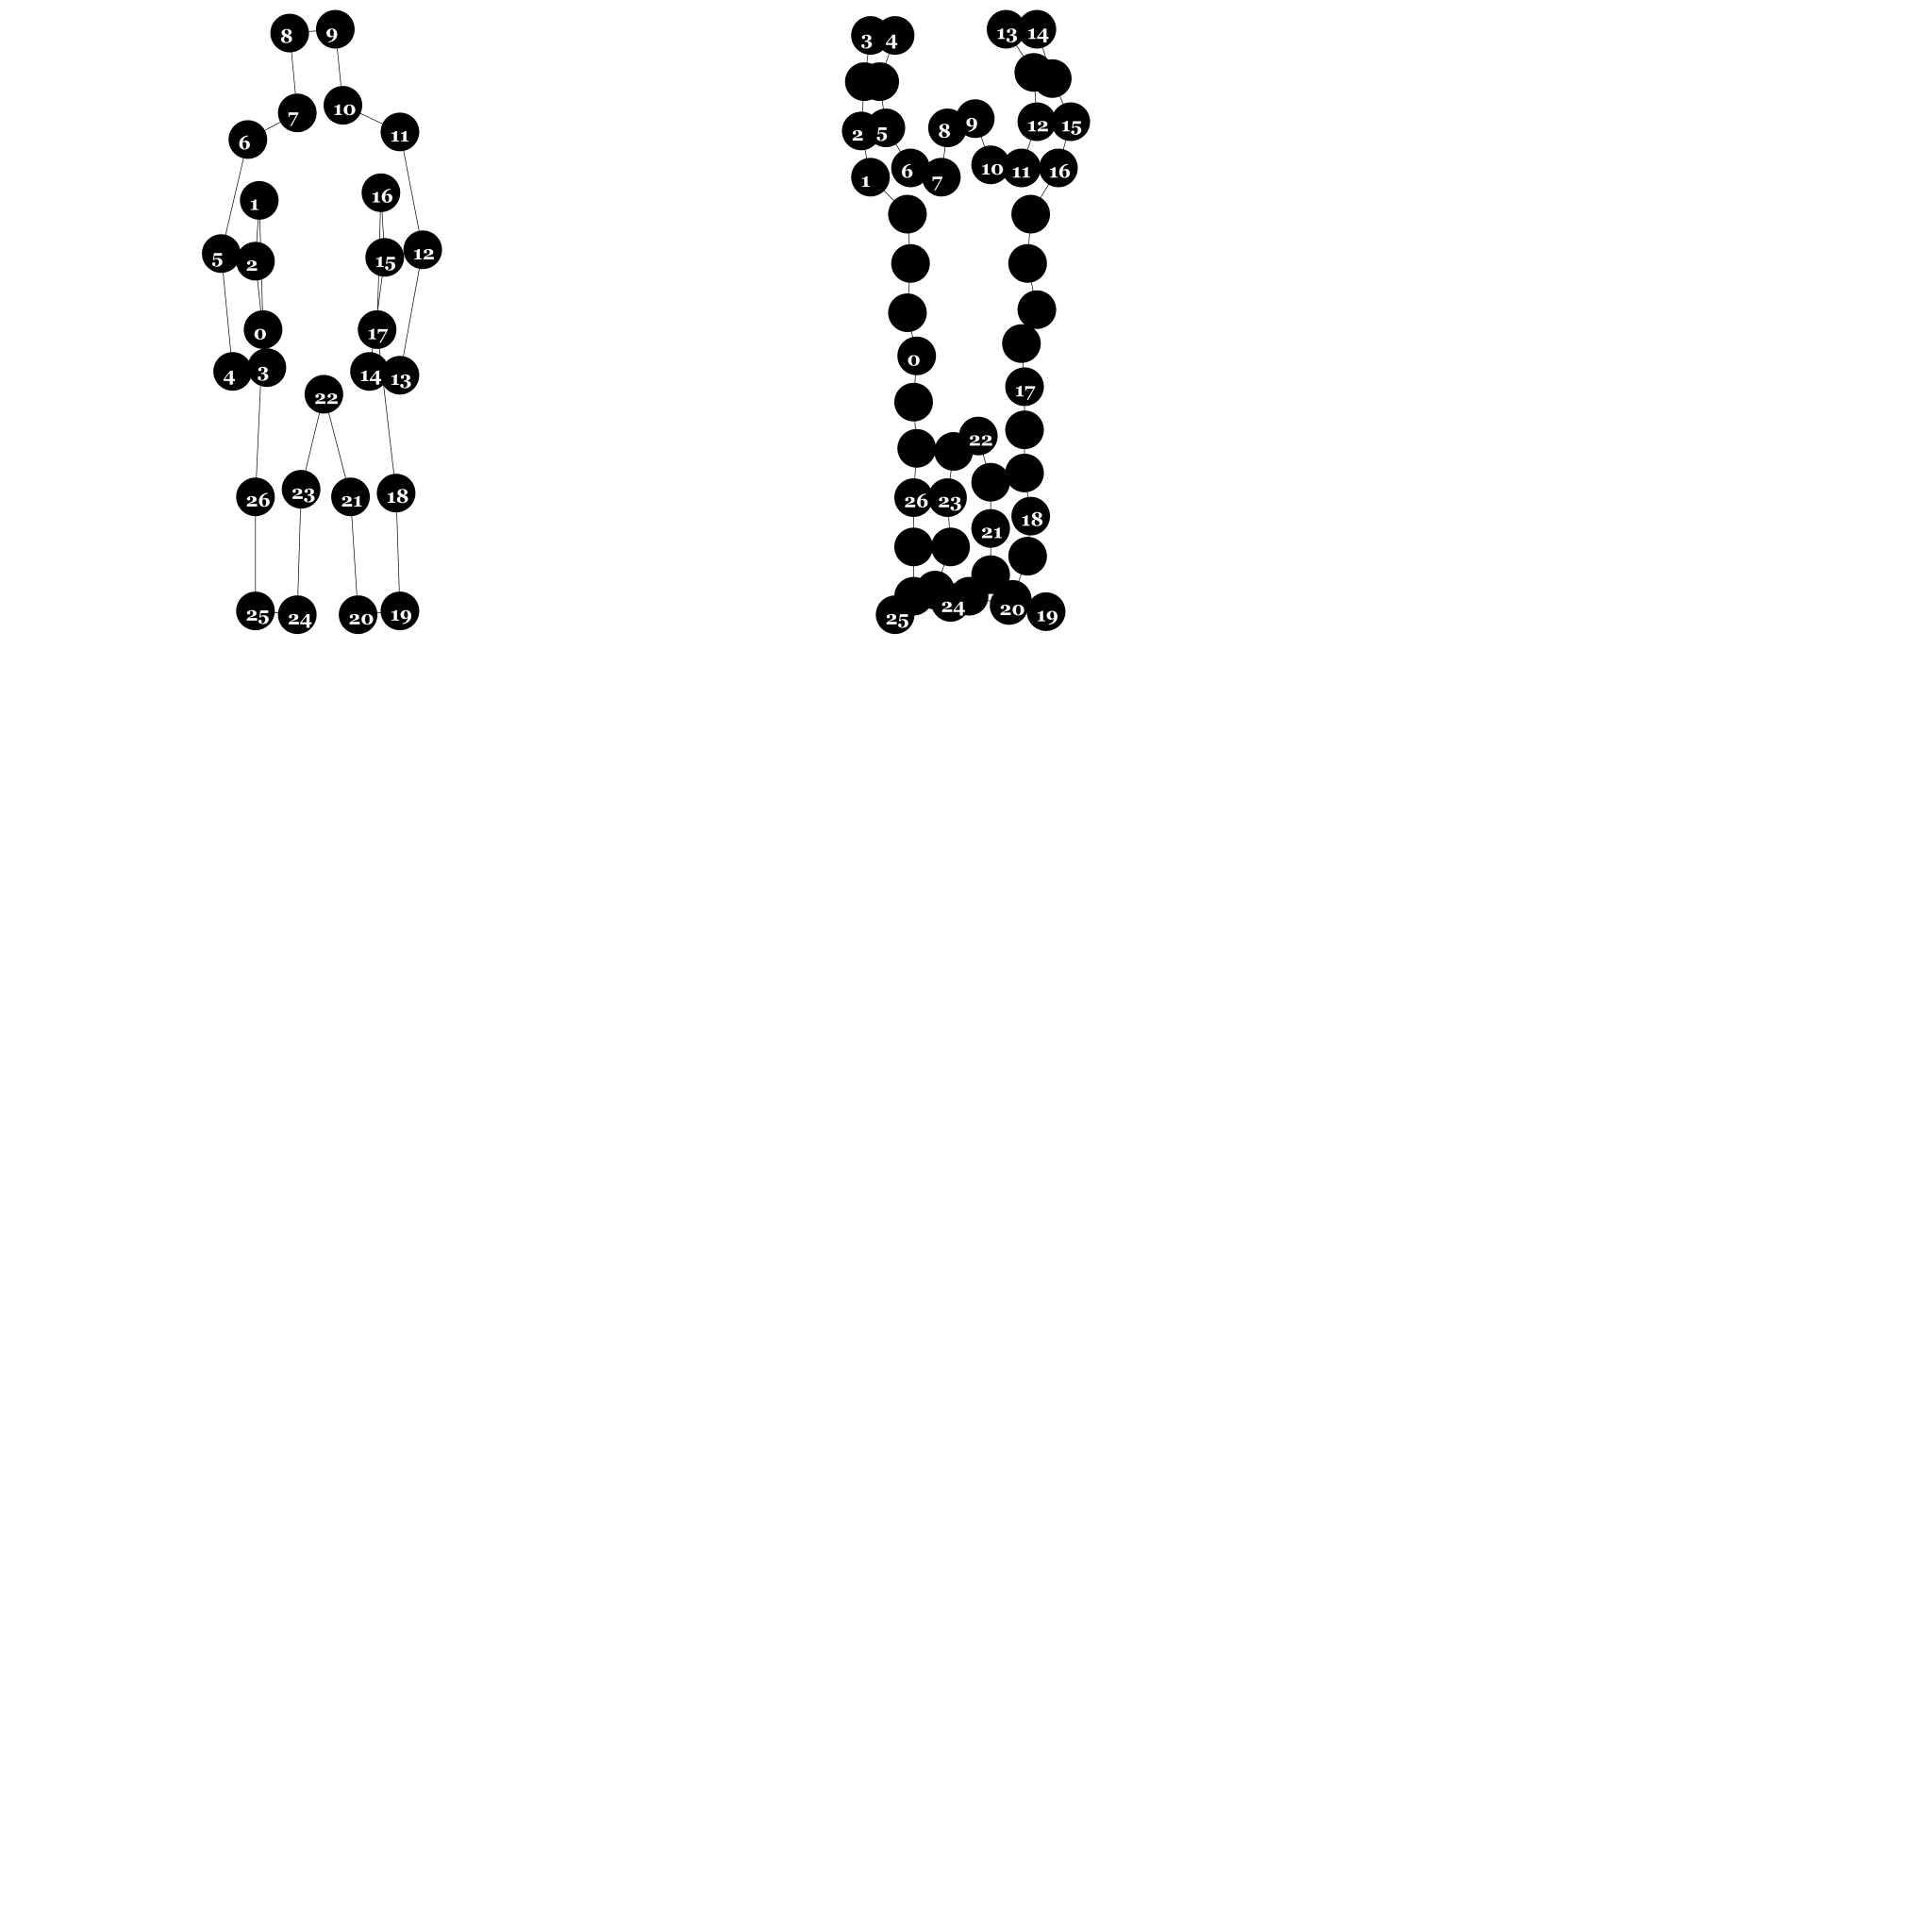
\includegraphics[width=6in]{./2.parsing/one_to_one/parse.eps}



  \section{Building a Grammar From a Single Curve}
    
\subsection{Building a Grammar for a Single Curve}
\label{sec-single}

The current work is based on \cite{hcm}, in which grammar-like
structures were constructed from single training curves. We follow
that approach here.

A grammar $\GGG_C$ for a curve $C$ should produce $C$, and curves
which look like $C$. We are not trying to achieve structural variation
yet, so the only variation that $\GGG_C$ needs to account for is:
\begin{itemize}
\item Slight geometric deformations of $C$
\item Curves like $C$ that have more or fewer sample points.
\end{itemize}
We model geometric deformations with the nonparametric distribution
described in Section \ref{sec-deform}. We model curves with fewer sample
points by allowing every nonterminal $X$ to have the rule $[X\to
\ell]$. We initially set the probability of this rule based on the
scale of $X$, as described in Section \ref{sec-scale}.

The nonterminals of our grammar will correspond to subcurves of $C$.
We model curves with more sample points than $C$ by allowing any
nonterminal $X$ that arises from a subcurve of length $1$ to have two
rules:
\begin{itemize}
\item $X\to \ell$
\item $X\to XX$
\end{itemize}
The second rule is infinitely recursive, and thus allows the curve to
get arbitrarily long.
  \marginnote{Our current thinking is to have the
  probability of $X\to XX$ be chosen in the same scale-dependent way
  as the probability of $X\to YZ$. But this might be problematic.}

\subsection{General Case}

Let $C$ be a curve of length $n$. A \emph{generic parse tree} for $C$
is a parse tree that does not refer to any particular grammar. This
will just be a binary tree $T$ where each node is labeled by an
interval $(i,j)$, $0\le i < j \le n$, and
\begin{itemize}
\item The root of $T$ is $(0,n)$
\item If $(i,j)$ is a node, and $j-i \ge 2$, then $(i,j)$ has exactly
  two children, and they are of the form $(i,k)$ and $(k,j)$ for some
  $k$.
\item $T$ has $n$ leaf nodes $(i,i+1)$ for $i=0,\dots,n-1$.
\end{itemize}

We can then specify a simple grammar for $C$ that produces the parse
tree $T$. For every node $(i,j)$ in $T$, $\GGG$ has a nonterminal
$X^{(i,j)}$. When $(i,j)$ has children $(i,k)$ and $(k,j)$, $\GGG$ has
a rule $[X^{(i,j)} \to X^{(i,k)}X^{(k,j)}]$. The scale of the
nonterminal $X^{(i,j)}$ is $\frac{j-i}{n}$ (see Section \ref{sec-scale}).

Our choice of an initial grammar for $C$ is thus based on choosing a
generic parse for $C$. Some choices:
\begin{enumerate}
\item An arbitrary parse, chosen to make the tree as balanced as
  possible. This approach corresponds most closely to that of
  \cite{hcm}.
\item A parse that has been chosen to respect the structure of
  $C$. This approach would require us to identify natural constituents
  of curves. There has been some work on this question.
\item We can choose multiple parses, and create a grammar that can
  parse $C$ in multiple ways. 
\end{enumerate}

Our favored approach is number 3. We want to create a small grammar
that can parse $C$ in as many ways as possible, so that the EM
retraining can discover the ``correct'' sub-grammar. To this end, we
use the sparse decomposition families of Section
\ref{sec-fast-parsing}.






  \section{Models of Triangle Deformation}
    
\marginnote{beginning of models/triangle.tex}

\subsection{Procrustes Distance and The Watson Distribution}
\marginnote{Write this!}

\subsection{Non-Parametric Deformation Model}

When sampling from our grammar, we place a midpoint $q$ according to
the midpoint distribution $\mu_{X\to YZ}(q; p, r)$, where $X_{p,r}$ is
the placed symbol we are currently replacing.

We want our grammar to be invariant to translation, scale, and
rotation. Therefore, we translate, scale, and rotate $\RR^2$ with a
map $\phi$ such that $\phi(p) =(0,0)$ and $\phi(r) =(1,0)$, and
represent $q$ via the coordinates $\widehat{q} = \phi(q)$.

In this coordinate system, we use the nonparametric distribution given
by the Parzen windows method \cite{parzen}. If we have seen samples
$q_1, \dots, q_k$, then
$$\mu_{X\to YZ}(q ; p, r) = \frac{1}{n} \sum_{i=1}^{k}
\frac{1}{2\pi h^2} e^{\frac{\| \widehat{q_i} - \widehat{q}\|^2}{2h^2}}.$$

In the context of kernel density estimators, the parameter $h$ is
called the bandwidth. It specifies how much smoothing to apply to the
density estimation. Selecting a suitable bandwidth is often
problematic. 

It is worth noting that this nonparametric distribution is just a
mixture of Gaussians, and thus there is no solid distinction between a
mixture of multiple copies of the rule $X\to YZ$ with Gaussian
midpoint distributions, and a single copy with a mixture of Gaussians
midpoint distribution. We will prefer the second, since the resulting
grammar has a simpler structure, as discussed in Section \ref{sec-mdl}.


\subsection{Open Questions}

Which shape grammars can be converted to Chomsky Normal Form?

This is not as straightforward as the corresponding question for
traditional context-free grammars, since not all control point
distributions can be expressed as products of midpoint
distributions. Recursion makes this question more subtle.

\newthought
Process Model of Continuous Curves

We can imagine a shape grammar which does not have any terminal
$\ell$, but rather continues to generate sample points forever. If
such a grammar is finite, it would have to have recursive rules to
allow an infinite number of expansions. The simplest case would be
rules of the form $L\to LL$.

If we have a grammar with only one symbol $L$, and only one rule $L\to
LL$, with $\mu_{L\to LL}(q;p,r)$ being the degenerate distribution
that only takes on the value $q=\half(p+r)$, then it is clear that we
generate only straight lines.

We can ask what conditions on the grammar are necessary to produce
smooth curves under such a model. For specificity, let us assume that
we represent our curve by a function $C(t) : [0,1] \to \RR^2$. Let
$C_k$ be the curve we obtain after $k$ rounds of substitution, and let
$C(\frac{i}{2^k}) = C_k[i]$. It can be checked that this gives the
same value for $\frac{i}{2^k}$ and $\frac{i'}{2^{k'}}$ when the two
are equal, and thus $C(\cdot)$ is well-defined.  Since the set
$\left\{\frac{i}{2^k}\right\}$ is dense in $[0,1]$, we can define
$C(t)$ for other values by continuity when $C(\cdot)$ is continuous.

Then, there are several interesting questions:

\begin{q}
What conditions on the grammar are necessary in order for $C(t)$ to
be continuous?
\end{q}

\begin{q}
What conditions on the grammar are necessary in order for $C(t)$ to
be smooth?
\end{q}

\begin{q}
Is it possible to write down a simple grammar for a simple parametric
curve such as a circle or a Bezier curve?
\end{q}

\begin{q}
Suppose that we generate a smooth curve $C(t)$ via a grammar \GGG, and
then subsample it to get a curve $C_*$ with a finite number of
points. How do we parse $C_*$ with \GGG, and how do we use this parse
to assign a likelihood to $C_*$ under \GGG?
\end{q}

\begin{q}
What is a good probabilistic interpretation of subsampling?
\end{q}

\marginnote{end of models/triangle.tex}

  \section{Dealing with Variation in Length}
    
\FloatBarrier

\section{Recover a correspondence where some points are missing}

Here we build a grammar from a ground-truth Romer curve, and try to
parse one of the (much shorter) hand-annotated Romer curves. We can
safely assume that every point in the parsed curve has a corresponding
one in the example curve, which is the reverse of the previous
experiments.

In order to do this successfully, the grammar needs shortening rules,
but not lengthening rules.

\begin{figure}
\includegraphics[width=\linewidth]{experiments/2.parsing/shorter_curves/output.d/parse_00.png}
\caption{On the left, the model curve. On the right, the parsed curve}
\end{figure}

This is really quite bad. We are using a pretty bad SDF to initialize
the grammar, so maybe that is why. Here is the SDF:

\includegraphics[width=5in]{experiments/2.parsing/shorter_curves/output.d/sdf_8.png}

It is somewhat troubling that it does this badly, though. Let us try
it again with less geometric variation.

\begin{figure}
\caption{On the left, the model curve. On the right, the parsed curve}
\includegraphics[width=6in]{experiments/2.parsing/shorter_curves/output.d/parse_80.png}
\end{figure}

This is basically correct, although the fine details are not very good
looking. This is probably because of the SDF. The shortening rules
only allow the parser to chop off constituents. If the constituents
look bad, then the parse will look bad.


    
\FloatBarrier

\section{Recover a correspondence with extra intermediate points}

We build a grammar from a single example from the hand-annotated Romer
dataset, and use it to parse a curve from the ground-truth Romer
dataset. We successfully recover a very reasonable correspondence.

\begin{figure}
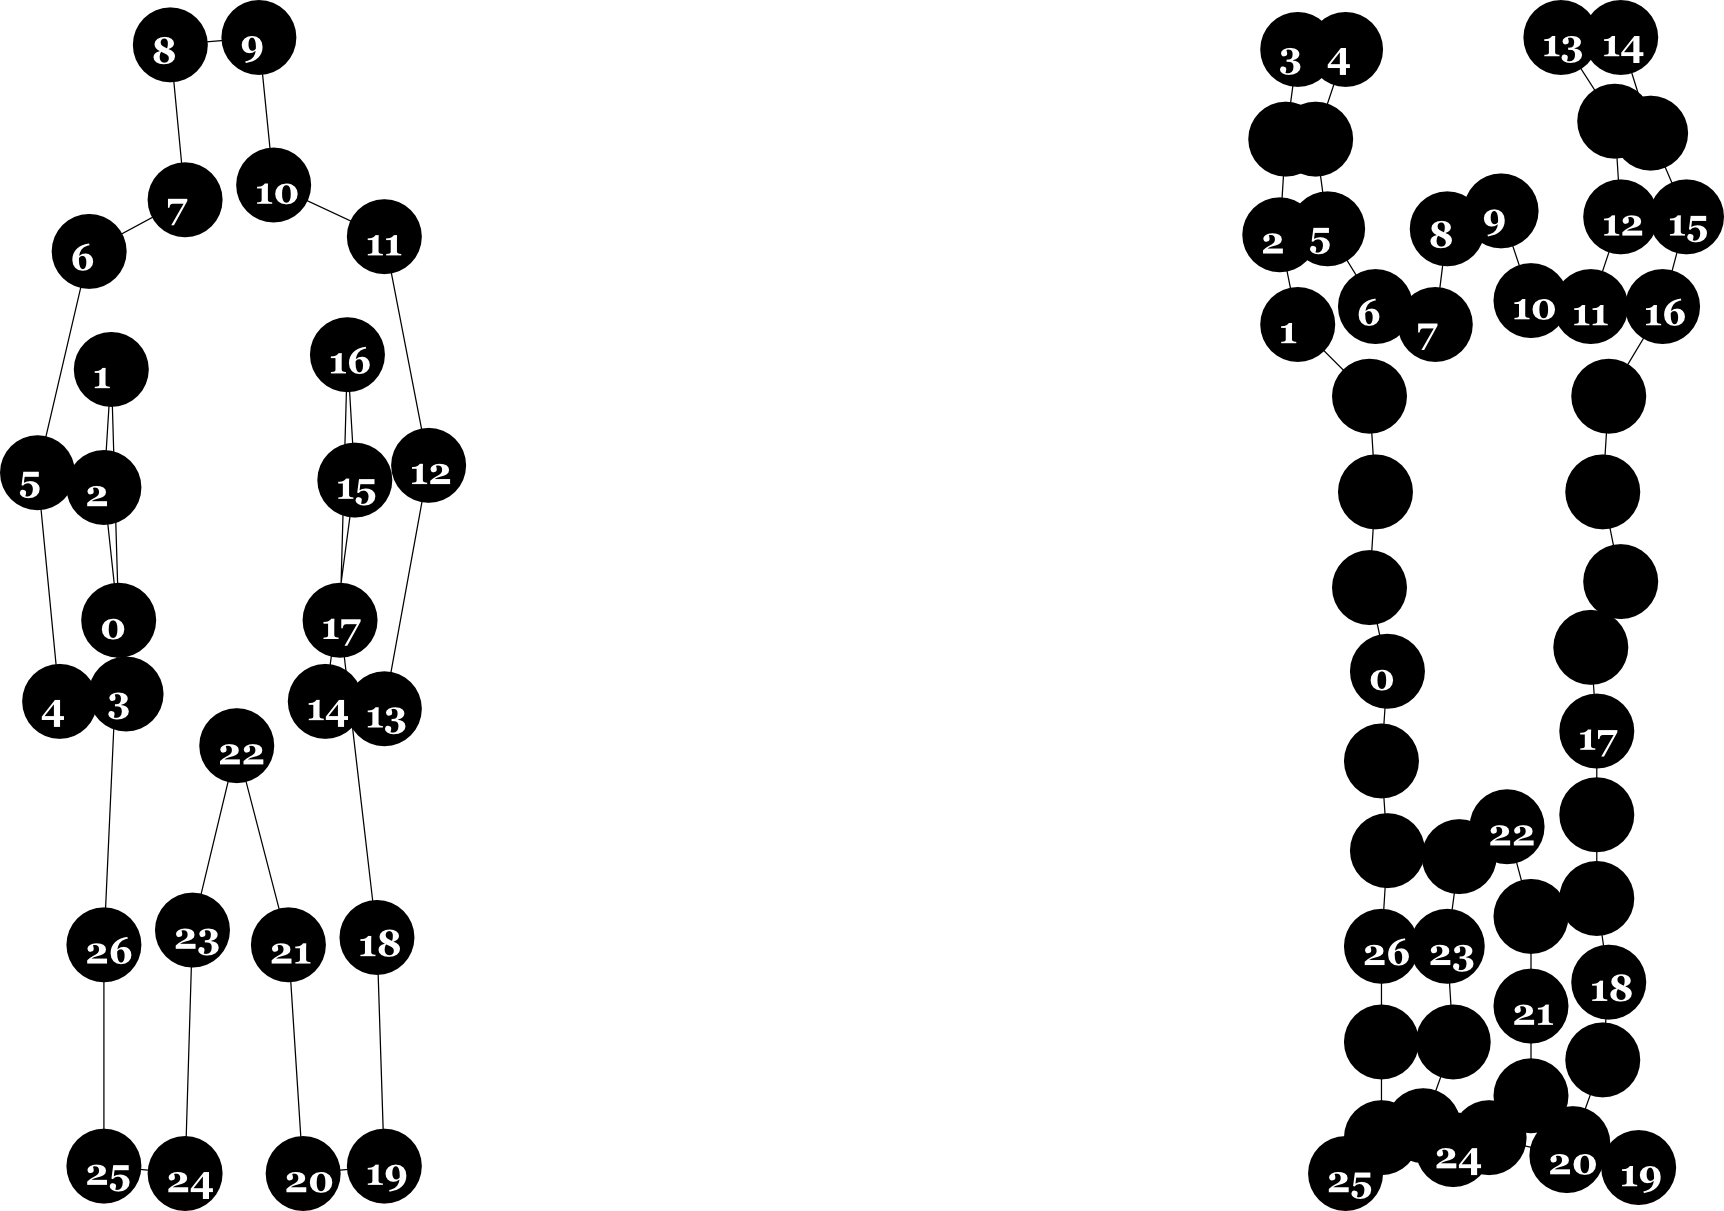
\includegraphics[width=\linewidth]{experiments/2.parsing/longer_curves/output.d/parse.png}
\caption{On the left, the model curve. On the right, the parsed curve}
\end{figure}

The ground-truth Romer curve has more intermediate points, so this
demonstrates that our grammar construction and parsing algorithm deal
well with additional intermediate points. The grammar must have
lengthening rules, but doesn't need shortening rules.



  \section{Sampling Experiments}

  \section{Classification Experiments}

  \section{Constellation Grammars}

\chapter{Detecting Objects in Cluttered Images}

  \section{Goals}
    
In \cite{hcm}, hierarchical curve models are used to find shapes in
cluttered images. The same thing can be done for our models.

We can test this out on the ETHZ dataset, which is relatively easy. We
could also try to find curves in the much harder LabelMe dataset.

\subsection{Parsing in Cluttered Images}
Given a shape model and an image containing a similar shape, we would
like to be able to find the shape in the image. This is done by
searching for a shape that is rated highly by the shape model, and for
which evidence exists in the image.

We will work on solving harder and harder versions of this problem:
  - Take a known curve, and generate evidence that suggests that
    curve, and no other curve. Find the curve.
  - As above, but randomly add evidence to other parts of the image.
  - Extract evidence from an actual image, and use this to find the
    curve.



  \section{Prior Work}

  \section{Motivating Examples}

  \section{Parsing Scenes}

  \section{Data Models for Object Detection}

  \section{Speeding up Detection with Filtrations}
    \marginnote{beginning of filtrations.tex}

\section{Lightest Derivation Problems}

We now discuss filtration parsing, which is a technique to speed up
parsing by eliminating unlikely parses from consideration. It is
similar in nature to \cite{astar}, but it can be applied in a more
general context. We first require some preliminaries.

\marginnote{Think about approximation guarantees for inadmissible
  homomorphisms. If the maximum size of a derivation is $N$, and
  $w(X\tne_v Y, Z) \ge w(\Phi(X) \tne \Phi(Y), \Phi(Z)) - \epsilon$,
  then we will find a derivation with cost at most $OPT +
  N\epsilon$. Similarly, if we stop when $\ell > u - \delta$, then we
  will find a derivation with cost at most $OPT + N\epsilon +
  \delta$.}

\marginnote{Discuss min-Bloom filters somewhere?}

We will write a binary tree with root node $v$, left subtree $T_1$,
and right subtree $T_2$ as $\tree{v}{T_1}{T_2}.$ We
will also have non-binary trees, which we will write as
$\treee{v}{T_1}{\dots}{T_k}$.

\begin{defn}
  Let $T_1, T_2$ be labeled binary trees, where $u$ is a leaf node of
  $T_1$ and $v$ is the root node of $T_2$. We define a new tree $T_1
  \triangle^{\cancel{u}}_v T_2$ to be the tree resulting from deleting
  $u$ and attaching $T_2$ in its place.
\end{defn}

A lightest derivation problem \cite{kld} is a tuple $(\SSS,\RRR)$, where $\SSS$
is a set of statements and $\RRR$ is a set of weighted inference
rules. We require that $\SSS$ contain $\perp$, a special
goal-statement. We will denote the weight of a rule $R\in \RRR$ by
$w(R)$.

The goal is to find the lightest (i.e., lowest cost) derivation of the
goal statement using the rules in $\RRR$. Our inference rules are of
the following form:
\begin{align*}
&A_1 : w_1\\
&\; \vdots \\
&A_k : w_k\\
&\infrul{v}\\
&C : v + w_1 + \dots + w_k.
\end{align*}
Here the antecedents $A_i$ and the conclusion $C$ are statements in
$\SSS$, $v$ is the cost of using the rule in a derivation, and $w_i$
is the cost of deriving $A_i$. We will also denote such a rule by
$\langle C \tne_v A_1, \dots, A_k \rangle$. We write the conclusion on
the left to maintain consistency with the conventional notation for
context-free grammars. Note that the antecedents $A_i$ are unordered,
so that $\langle C\tne_v A_1, A_2 \rangle$ and $\langle C_\tne_v A_2,
A_1 \rangle$ would be considered equivalent.

A derivation of $C$ is a finite tree whose root is labelled with a
rule $ \langle C\tne_v A_1, \dots, A_k \rangle$, where the subtree
rooted at the $i$-th child is a derivation of $A_i$. The leaves of
this tree are rules with no antecedents. The cost of a tree is the sum
of the costs of the rules at its nodes. We will denote the cost of a
tree $T$ by $wt(T)$.

Usually, we will work with lightest derivation problems that are in
Chomsky Normal Form, i.e., inference rules will either have two
antecedents,
\begin{align*}
  &A : w_A\\
  &B : w_B\\
  &\infrul{v}\\
  &C : v + w_A + w_B \\
  \intertext{in which case they will be called {\em binary rules}, or
    they will have no antecedents,}
  &\infrul{v}\\
  &A : v,
\end{align*}
in which case they will be called {\em lexical rules}.

We will be interested only in lightest derivation problems that are
acyclic. A lightest derivation problem $(\SSS,\RRR)$ is {\em acyclic}
if there is an ordering $\le$ of the statements in $\SSS$ such that,
for each rule $\langle C\tne_v A_1,\dots, A_k \rangle \in \RRR$, $A_i
\le C$ for $i=1,\dots, k$.

In most cases, the lightest derivation problem will be specified
implicitly by listing abstracts statements and rules which contain
free variables. The lightest derivation problem is then obtained by
substituting all possible values for each free variable in the
abstract statements and rules to create concrete statements and
rules. In such cases, listing all the inference rules may be
prohibitively slow.

As an example, we can consider CKY parsing with PCFG's as a lightest
derivation problem. Suppose our a grammar is in Chomsky Normal Form,
and we are parsing a string $s_1, \dots, s_n$. The lightest derivation
problem will have statements $X(i,j)$ for every nonterminal $X$ and
every pair of integers $i,j$ with $1\le i \le j \le n$. $X(i,j)$ will
represent the statement that nonterminal $X$ has the yield $s_i,\dots,
s_j$. The rules will be, for every binary rule $X\to YZ$ in the
grammar, and all $i,j,k$ with $1\le i \le j \le k \le n$,
\begin{align*}
&Y(i,j) : w_1\\
&Z(j+1,k) : w_2\\
&\infrul{w(X \to YZ)}\\
&X(i,k) : w_1 + w_2 + w(X \to YZ) \\
\intertext{and, for every nonterminal $X$, and for every $i$ such that the lexical rule $X\to s_i$ exists,}
&\infrul{w(X\to s_i)}\\
&X(i,i) : w(X\to s_i),
\end{align*}
The cost $w(X \to \lambda)$ will be the negative log of the transition
probability specified by the PCFG. The goal statement $\perp$ is in
this case $S(1,n)$, where $S$ is the start symbol of the grammar.

In this case, listing all the concrete inference rules requires
$O(mn^3)$ time, where $m$ is the number of productions in the
PCFG. This is the running time of the CKY algorithm, which is too slow
to use in many contexts.

\section{Solving Lightest Derivation Problems via Dynamic Programming}

Let $\Delta_{\SSS,\RRR}(C)$ be the set of derivations of $C$. We
define the {\em cost} of $C$ to be
$$cost_{\SSS,\RRR}(C) = \min_{T\in \Delta_{\SSS,\RRR}(C)} wt(T).$$

\begin{obs}
\label{prop-induct-inside}
Let $(\SSS,\RRR)$ be an acyclic\footnote{In the case of a cyclic
  lightest derivation problem, this definition would also allow
  infinite trees.}  lightest derivation problem. We can construct the
set $\Delta_{\SSS,\RRR}(C)$ recursively as follows:
$$
  \Delta_{\SSS,\RRR}(C) = \left\{
    \treee{\langle C\tne_v A_1, \dots, A_k\rangle}{T_1}{\dots}{T_k} \mid
    \langle C\tne_v A_1, \dots, A_k\rangle \in \RRR, T_i \in
    \Delta_{\SSS,\RRR}(A_i)  \right\}
$$
\end{obs}

\begin{obs}
  \label{obs-rec-inside}
  Let $(\SSS,\RRR)$ be an acylic lightest derivation problem.  We can
  recursively compute $cost_{\SSS,\RRR}(C)$ as
$$cost(C) = \min_{C\tne_v A_1,\dots, A_k} v + \sum_i cost(A_i).$$
\end{obs}

We can use Observation \ref{obs-rec-inside} in Algorithm
\ref{alg-inside}. We assume that $(\SSS,\RRR)$ is an acylic lightest
derivation problem in Chomsky Normal Form. Note that this is a
standard use of dynamic programming.

\begin{algorithm}
\caption{$lightest\_derivation(\SSS,\RRR)$}
\begin{algorithmic}
  \INPUT $\SSS, \RRR$
  \STATE{$COST \from \emptyset$}
  \STATE{$BEST \from \emptyset$}
  \FOR{$X\in \SSS$ (in $\le$ order)}
  \STATE $COST[X] \from \infty$
  \FOR{$\langle X\tne_v\rangle \in \RRR$}
  \IF{$COST[X] > v$}
  \STATE $COST[X] \from v$
  \STATE $BEST[X] \from \langle X\tne_v \rangle$
  \ENDIF
  \ENDFOR
  \FOR{$\langle X\tne_v YZ \rangle \in \RRR$}
  \STATE $new \from COST[Y] + COST[Z] + v$
  \IF{$new < COST[X]$}
  \STATE $COST[Z] \from new$
  \STATE $BEST[Z] \from \langle X\tne_v YZ \rangle$
  \ENDIF
  \ENDFOR
  \ENDFOR
  \RETURN $COST, BEST$
\end{algorithmic}
\label{alg-inside}
\end{algorithm}

\subsection{Contexts}

In this section, we define ``contexts'', which are a sort of dual
concept to derivations. See also \cite{astar}.

\marginnote{How do you represent a single-node tree? If not in CNF,
  don't necessarily know how many children a node ``should'' have.}
\begin{defn}
  A $B$-context for $C$ is either the single-node tree
  $\frac{hole(C)}{\cdot}$ if $B=C$, or a finite tree whose root is
  labelled with a rule $ \langle B \tne_v A_1,\dots, A_k \rangle$,
  where the subtree rooted at the $i$-th child is either a derivation
  of $A_i$ or an $A_i$-context for $C$, and exactly one of the
  subtrees is an $A_i$-context rather than a derivation. The cost of a
  context $T$ (denoted $wt(T)$) is the sum of the cost of the rules at
  all of its nodes. Note that the node labelled $hole(C)$ has cost
  $0$.
\end{defn}

Let $\Gamma_{\SSS,\RRR}(C)$ be the set of $\perp$-contexts of $C$. Define
$$ocost_{\SSS,\RRR}(C) = \min_{T\in \Gamma_{\SSS,\RRR}(C)} wt(T).$$
$ocost$ is analogous to the outside cost in the Inside-Outside
Algorithm for PCFG's, but here we are trying to find a lightest
derivation rather than sum over all derivations.

\marginnote{Figure to illustrate this prop?}
\marginnote{Assuming CNF here}
\begin{obs}
\label{prop-outer-set}
Let $(\SSS,\RRR)$ be an acylic lightest derivation problem.
We can construct the set $\Gamma_{\SSS,\RRR}(C)$ recursively as follows:
\begin{itemize}
\item $\Gamma_{\SSS,\RRR}(\perp) = \left\{ \frac{hole(\perp)}{\cdot}
  \right\}$. (Note that, since the lightest derivation problem is
  assumed to be acyclic, this is the only $\perp$-context for $\perp$.
\item $\Gamma_{\SSS,\RRR}(X) = \left\{ \treee{\langle X \tne_v
      A_1,\dots, A_k \rangle}{T_1}{\dots}{T_k} \mid \mbox{exactly one
    }T_i \in \Gamma_{\SSS,\RRR}(C,A_i), \mbox{ other } T_i \in
    \Delta_{\SSS,\RRR}(A_i) \right\}$
\end{itemize}
\end{obs}

\begin{obs}
\label{obs-outside}
Given $cost(X)$ for all $X$, we can recursively compute $ocost(X)$:

\begin{align*}
ocost(\perp) &= 0\\
ocost(C) &= \min_{A\tne_v C,B_1,\dots,B_{k-1}\in \RRR} ocost(A) + v + \sum_i cost(B_i)\\
\end{align*}

This is implemented by Algorithm \ref{alg-outside}.
\end{obs}

\begin{algorithm}
\caption{$outside(\SSS,\RRR,COST)$}
\begin{algorithmic}
  \INPUT{$\SSS, \RRR, COST$}
  \STATE $OCOST \from \emptyset$
  \STATE $OCOST[\perp] \from 0$
  \FOR{$X\in \SSS$ (in reverse $\le$ order)}
  \FOR{$X\tne_v YZ \in \RRR$}
  \STATE $OCOST[Y] \from \min \{ OCOST[Y], v + OCOST[X] + COST[Z]\}$
  \STATE $OCOST[Z] \from \min \{ OCOST[Z], v + OCOST[X] + COST[Y]\}$
  \ENDFOR
  \ENDFOR
  \RETURN $OCOST$
\end{algorithmic}
\label{alg-outside}
\end{algorithm}


\section{Homomorphisms}

\begin{defn}[Homomorphism]
\marginnote{Should we change the name? ``minimorphism''?}
\marginnote{Do we require that $\Phi(\perp) = \perp$?}
  A {\em homomorphism} of lightest derivation problems is a function
  $\Phi : \SSS \to \SSS'$ such that, for every $\langle C \tne_v A_1,
  \dots, A_k \rangle \in \RRR$, there exists a rule $\langle \Phi(C)
  \tne_w \Phi(A_1), \dots, \Phi(A_k)\rangle\in \RRR'$, with $w\le v$.
\end{defn}
Homomorphisms are called ``abstractions'' in \cite{astar}.

\begin{lem}
  Let $\Phi$ be a homomorphism of lightest derivation problems. Then
  $cost_{\SSS,\RRR}(X) \ge cost_{\SSS',\RRR'}(\Phi(X))$. Also, 
  $ocost_{\SSS,\RRR}(X) \ge ocost_{\SSS',\RRR'}(\Phi(X))$.
\end{lem}
\begin{proof}
  Let $T$ be the derivation achieving $cost(\SSS,\RRR)(X)$. We can
  replace each rule $\langle C\tne_v A_1, \dots, A_k \rangle$ used in
  the derivation with a rule $\langle \Phi(X) \tne_w \Phi(A_1), \dots
  \Phi(A_k) \rangle$, thereby creating a valid derivation of $\Phi(X)$
  whose total cost is lower than that of $T$. Thus the lightest
  derivation of $\Phi(X)$ also has cost lower than that of $T$.
\end{proof}

\begin{defn}
Let $(\SSS,\RRR)$ be a lightest derivation problem. A table $C$
mapping statements to weights is a {\em valid lower bound} for
$(\SSS,\RRR)$ if, for every $X\in \SSS$, $cost_{(\SSS,\RRR)} \ge
C[X]$.
\marginnote{Also define valid lower bound on contexts}
\end{defn}

\begin{lem}
  If $\Phi:\SSS \to \SSS'$ is a homomorphism, and $C'$ is a valid
  lower bound for $(\SSS',\RRR')$, and we define $C[X] :=
  C'[\Phi(X)]$, then $C$ is a valid lower bound for $(\SSS,\RRR)$. $C$
  is called the {\em pullback} of $C'$ under $\Phi$.
\end{lem}
\begin{proof}
  Let $X\tne A_1,\dots, A_k$ be the rule that achieves $X$'s lightest
  derivation. Then
\begin{align*}
 cost_{\SSS,\RRR}(X) &\ge cost_{\SSS',\RRR'}(\Phi(X))\\
\intertext{by some proposition}
 &\ge C'[\Phi(X)] \\
\intertext{because $C'$ is a valid lower bound for $\SSS',\RRR'$}
 &= C[X]
\end{align*}
\end{proof}

\begin{obs}
  Every derivation of $\perp$ in which $X$ appears can be realized as
  $T_1 \triangle^{\cancel{hole(X)}} T_2$, where $T_1\in \Gamma_X$ and
  $T_2\in \Delta_X$. Therefore, if $cost(X) = \min_{T\in \Delta_X}
  wt(T)$ and $ocost(X) = \min_{T\in \Gamma_X}$, then the lightest
  derivation of $\perp$ using $X$ has cost $cost(X) + ocost(X)$.
\end{obs}

\begin{lem}
  If $T$ is a lightest derivation of $\perp$, and $X$ does not appear
  in $T$, then the value of $\SSS,\RRR$ is the same as the value of
  $\SSS\sm \{X\}, \RRR'$, where $\RRR'$ has no rules involving $X$.
\end{lem}


\marginnote{Use COST, OCOST in pseudocode to make them look more like
  data structures. Maybe somehow also emphasize that they are lower
  bounds. $\underline{COST}$?}

\section{Filtration Parsing}


\begin{thm}
\label{thm-filt-test}
  Let $(\SSS,\RRR)$ be a lightest derivation problem, and let $X$ be a
  statement. Suppose that $\underline{COST}$ is a valid lower bound
  for $(\SSS,\RRR)$, and $\underline{OCOST}$ is a valid lower bound on
  contexts for $(\SSS,\RRR)$. Then the lightest derivation that uses
  $X$ has cost at least $\underline{COST}[X] + \underline{OCOST}[X]$.

  Consequently, if there is a derivation $T$ with cost $u <
  \underline{COST}[X] + \underline{OCOST}[X]$, then no lightest
  derivation of $\perp$ uses $X$.
\end{thm}

We can use this theorem to perform an admissible coarse-to-fine search
strategy. This is implemented by Algorithms \ref{alg-filt-inside},
\ref{alg-filt-outside}, and \ref{alg-filt}. Algorithms
\ref{alg-filt-inside} and \ref{alg-filt-outside} are very similar to
Algorithms \ref{alg-inside} and \ref{alg-outside}, but they do not
consider solutions that violate the lower bound of Theorem
\ref{thm-filt-test}.

Algorithm \ref{alg-filt} shows how to use the inside pass and the
outside pass to organize our search. The lifting procedure $lift$ and
the modification of $\Phi$ must be customized to the problem
domain. The lifting procedure will generally be a standard
coarse-to-fine strategy, where we search at higher and higher levels
of detail, always limiting ourselves to parses consistent with the
solution found at the previous, coarser level.

Our modification of $\Phi$ is chosen to increase the level of detail
at statements similar to those used in the last candidate parse. This
allows us to focus in on regions that could plausibly contain an
object of interest without spending extra time in other regions. Thus,
filtration parsing can be considered an attention-based method. This
technique is similar to Coarse-to-Fine Dynamic Programming (CFDP)
\cite{cfdp}, but is applicable to a broader class of problems than
CFDP, which is limited to finding the shortest path through a trellis
graph.

\begin{algorithm}
\caption{$inside(\SSS,\RRR,\underline{OCOST},u)$}
\begin{algorithmic}
  \INPUT $\SSS, \RRR, \underline{OCOST}$, $u$
  \STATE{$\underline{COST} \from \emptyset$}
  \STATE{$BEST \from \emptyset$}
  \FOR{$X\in \SSS$}
  \STATE $\underline{COST}[X] \from \infty$
  \FOR{$\langle X\tne_v \rangle \in \RRR$}
  \IF{$\underline{COST}[X] > v$}
  \STATE $\underline{COST}[X] \from v$
  \STATE $BEST[X] \from X\tne_v$
  \ENDIF
  \ENDFOR
  \ENDFOR
  \FOR{$X\in \SSS$ (in $\le$ order)}
  \IF{$\underline{COST}[X] + \underline{OCOST}[X] > u$}
  \STATE continue
  \ENDIF
  \FOR{$Z\tne_v XY \in \RRR$}
  \IF{$\underline{COST}[Y] + \underline{OCOST}[Y] > u$ or $\underline{COST}[Z] + \underline{OCOST}[Z] > u$}
  \STATE continue
  \ENDIF
  \STATE $new \from \underline{COST}[X] + \underline{COST}[Y] + v$
  \IF{$new < \underline{COST}[Z]$}
  \STATE $\underline{COST}[Z] \from new$
  \STATE $BEST[Z] \from Z\tne_v XY$
  \ENDIF
  \ENDFOR
  \ENDFOR
  \RETURN $\underline{COST}, BEST$
\end{algorithmic}
\label{alg-filt-inside}
\end{algorithm}


\marginnote{Are we forgetting something here? }
\begin{algorithm}
\caption{$outside(\SSS,\RRR,\underline{COST},u)$}
\begin{algorithmic}
  \INPUT{$\SSS, \RRR, \underline{COST}$, $u$}
  \STATE $\underline{OCOST} \from \emptyset$
  \STATE $\underline{OCOST}[\perp] \from 0$
  \FOR{$X\in \SSS$ (in reverse $\le$ order)}
  \IF{$\underline{COST}[X] + \underline{OCOST}[X] > u$}
  \STATE continue
  \ENDIF
  \FOR{$X\tne_v YZ \in \RRR$}
  \STATE $\underline{OCOST}[Y] \from \min \{ \underline{OCOST}[Y], v + \underline{OCOST}[X] + \underline{COST}[Z]\}$
  \STATE $\underline{OCOST}[Z] \from \min \{ \underline{OCOST}[Z], v + \underline{OCOST}[X] + \underline{COST}[Y]\}$
  \ENDFOR
  \ENDFOR
  \RETURN $\underline{OCOST}$
\end{algorithmic}
\label{alg-filt-outside}
\end{algorithm}

\marginnote{lift is getting incorrect parameters}
\marginnote{refer to definition of pullback}
\begin{algorithm}
\caption{Overall algorithm}
\begin{algorithmic}
  \STATE $l \from \infty$
  \STATE $u \from \infty$
  \STATE $\underline{OCOST}[*] = - \infty$
  \WHILE{$l < u$}
  \STATE $\underline{COST},BEST \from inside(u, \SSS, \RRR, \underline{OCOST})$
  \STATE $ctfcost, ctfsoln \from lift(\underline{COST},BEST)$
  \STATE $u \from \min(u, ctfcost)$
  \STATE Choose $\Phi_1, \Phi_{new}$ such that $\Phi = \Phi_1 \circ \Phi_{new}$.
  \STATE $\underline{COST} \from pullback(\Phi_1,\underline{COST})$
  \STATE $\underline{OCOST} \from outside(\SSS,\RRR,u, \underline{COST})$
  \ENDWHILE
\end{algorithmic}
\label{alg-filt}
\end{algorithm}

\section{Plane Parsing}

For the problem of detecting an object with a grammar in a cluttered
image, we have the following lightest derivation problem: for every
pair of points $p,q$, and every nonterminal $X$, we have the statement
$X(p,q)$. 

For every rule $X\to YZ$ in our grammar, and every triple of points
$p,q,r$, we have
\begin{align*}
&Y(p,q) : w_1\\
&Z(q,r) : w_2\\
&\infrul{v=-\log \left(\mu_{X\to YZ}(p,q,r) \cdot \rho(X \to YZ)\right)}\\
&X(p,r) : w_1 + w_2 + v \\
\intertext{and, for every rule $X \to \ell$, and every pair $p,q$}
&\infrul{v = data(p,q) -\log \rho(X\to \ell)}\\
&X(p,q) : v
\end{align*}
where $data(p,q)$ is a data cost modeling the log-likelihood of a line
segment existing between $p$ and $q$. Specifically, $data(p,q)$ is
chosen so that the sum over all terms will be $\log \frac{P(I\mid
  \mbox{parse})}{P(I\mid \mbox{no object})}$, where $I$ is the image
data and the probabilities refer to a probabilistic model of image
formation. Our image formation model is described in the next section.

Note that this lightest derivation problem is only acyclic if the
grammar used is acyclic. If the grammar used has cycles, we can
require that some rules $X(p,r)\tne_v Y(p,q), Z(q,r)$ are restricted
to $p,q,r$ such that the distance between $p$ and $r$ is at least as
big as that between $p$ and $q$, and $q$ and $r$.

We construct homomorphisms for filtration parsing by coarsening the
image grid, which we represent by pairs of integer indices.  Let
$\varphi((i,j)) = \left(\left\lfloor \frac{i}{2} \right\rfloor,
  \left\lfloor \frac{j}{2} \right\rfloor \right)$, and let
$\Phi(X(p,q)) = X(\varphi(p),\varphi(q))$. By repeatedly applying
$\Phi$, we construct a hierarchy of lightest derivation problems, in
which each level has 16 times fewer statements and (roughly) 64 times
fewer rules than the previous level.

To make the $\Phi_i$ be legitimate homomorphisms, for each rule
$X(p,r) \tne_v Y(p,q), Z(q,r)$ in $\RRR_i$, we need a lower bound on
the cost of rules mapping to it.


\marginnote{Talk about inadmissible methods too.}
\marginnote{Mention that this can be considered an attention-based method.}

\marginnote{end of filtrations.tex}

  \section{The Problem of Unintended Reuse}

  \section{Experimental Results}
% \section{Finding an obvious curve}

We build a grammar from a single curve, using a hand-picked
decomposition.


\includegraphics[width=4in]{experiments/4.images/standard_cky/output.d/examples.png}

We then pick some other curves which we wish to parse:

\includegraphics[width=4in]{experiments/4.images/standard_cky/output.d/targets.png}

We build a simple network on a 16x16 grid. We give curve segments a
data cost of 1.0, and short non-curve segments a data cost of 100.0.
On the left are the points of the network, with the curve segments
shown. On the right is the parse found.

\begin{center}
\begin{tabular}{ll}
\hline
 \includegraphics[width=10em]{experiments/4.images/standard_cky/output.d/network.0000.eps}  &
 \includegraphics[width=10em]{experiments/4.images/standard_cky/output.d/cky.im0000.final.png}  \\
\hline
 \includegraphics[width=10em]{experiments/4.images/standard_cky/output.d/network.0010.eps}  &
 \includegraphics[width=10em]{experiments/4.images/standard_cky/output.d/cky.im0010.final.png}  \\
\hline
\end{tabular}
\end{center}


% \section{Fuzzy parsing}

\begin{center}
\begin{tabular}{ll}
\hline
 \includegraphics[width=10em]{./4.images/fuzzy_cky/output.d/network.0000.eps}  &  \includegraphics[width=10em]{./4.images/fuzzy_cky/output.d/0000.yield.x8.final.eps}  \\
\hline
 \includegraphics[width=10em]{./4.images/fuzzy_cky/output.d/network.0010.eps}  &  \includegraphics[width=10em]{./4.images/fuzzy_cky/output.d/0010.yield.x8.final.eps}  \\
\hline
 \includegraphics[width=10em]{./4.images/fuzzy_cky/output.d/network.0020.eps}  &  \includegraphics[width=10em]{./4.images/fuzzy_cky/output.d/0020.yield.x8.final.eps}  \\
\hline
 \includegraphics[width=10em]{./4.images/fuzzy_cky/output.d/network.0030.eps}  &  \includegraphics[width=10em]{./4.images/fuzzy_cky/output.d/0030.yield.x8.final.eps}  \\
\hline
\end{tabular}
\end{center}




\begin{center}
\begin{tabular}{ll}
\hline
 \includegraphics[width=10em]{./4.images/fuzzy_cky/output.d/network.0040.eps}  &  \includegraphics[width=10em]{./4.images/fuzzy_cky/output.d/0040.yield.x8.final.eps}  \\
\hline
 \includegraphics[width=10em]{./4.images/fuzzy_cky/output.d/network.0050.eps}  &  \includegraphics[width=10em]{./4.images/fuzzy_cky/output.d/0050.yield.x8.final.eps}  \\
\hline
 \includegraphics[width=10em]{./4.images/fuzzy_cky/output.d/network.0060.eps}  &  \includegraphics[width=10em]{./4.images/fuzzy_cky/output.d/0060.yield.x8.final.eps}  \\
\hline
\end{tabular}
\end{center}

% \section{Parsing actual images}

We build a grammar using a hand-chosen annotation of this curve:

\includegraphics[width=10em]{./4.images/standard_cky/output.d/examples.eps}

Here is the image we wish to parse
%\% \includegraphics[width=10em]{../IMG0000.eps}

Here is the set of line segments allowable during parsing. Cheaper
curves are darker red.

\includegraphics[width=10em]{./4.images/image_parsing/output.d/network.0000.eps}

Here is the curve found during parsing:

\includegraphics[width=10em]{./4.images/image_parsing/output.d/0000.yield.final.eps}


\chapter{Parameter Learning for Grammatical Models}

  \section{Goals}
    % plans.tex

\marginnote{beginning of learning/learning\_goals.tex}

\subsection{Grammatical Learning Goals}

To test whether we can learn grammars, we propose a series of tasks on
real and synthetic data. The tests will have to be fairly qualitative,
although we hope that the models generated will give better results in
some quantitative task.

\subsection{Modeling Geometric Deformation}

Our first goal is to improve upon the results of \cite{hcm} by having
a more accurate model of geometric deformation. Since we have a
complete probabilistic model and a learning algorithm, this should be
possible.

The easiest version of this task is to generate good-looking samples
from the Articulator (Figure \ref{fig-articulator}). To make this task
even easier, we can start by training on bracketed samples, where we
specify that certain subcurves are constituents.

A harder version of this task is trying to generate good-looking
samples from the Romer dataset (Figure \ref{fig-romer}) and the
Weizmann Horse dataset (Figure \ref{fig-horse}). Here too we could
start with bracketed samples, although this will be more arbitrary for
silhouettes of people and horses.

\subsection{EM}
Given a fixed grammar structure (the symbols and rules), we can
optimize the parameters (rule probabilities and midpoint
distributions). EM is an iterative algorithm for improving the
parameters of a probabilistic model when important information (in our
case, the "true" parses) is unobserved.

We wish to demonstrate that EM works to tune the parameters of a shape
grammar. We would like to do the following:
  - Tune a simple hand-built grammar using several curves of fixed
    length, and then show that it produces reasonable samples, and
    that the cross-entropy estimated on unseen data is improved by EM.

  - Tune a simple hand-built grammar using several curves of fixed
    length. Start with a grammar that has several choices of midpoint
    for each of its rules, to allow for greater geometric
    variation. Show that it produces reasonable samples, and that the
    cross-entropy estimated on unseen data is improved by EM.

    We would also like to do this for a slightly more complicated
    grammar, in which the choice of midpoint at a high level can
    influence the choice of midpoint at lower levels.

  - Tune a hand-built grammar that exhibits structural variation.

  - We would like to show that EM does badly when it starts with bad
    parses.

\marginnote{end of learning/learning\_goals.tex}


  \section{Prior Work}

  \section{Motivating Examples}

  \section{Learning a Model of Triangles}
    
\marginnote{beginning of models/triangle.tex}

\subsection{Procrustes Distance and The Watson Distribution}
\marginnote{Write this!}

\subsection{Non-Parametric Deformation Model}

When sampling from our grammar, we place a midpoint $q$ according to
the midpoint distribution $\mu_{X\to YZ}(q; p, r)$, where $X_{p,r}$ is
the placed symbol we are currently replacing.

We want our grammar to be invariant to translation, scale, and
rotation. Therefore, we translate, scale, and rotate $\RR^2$ with a
map $\phi$ such that $\phi(p) =(0,0)$ and $\phi(r) =(1,0)$, and
represent $q$ via the coordinates $\widehat{q} = \phi(q)$.

In this coordinate system, we use the nonparametric distribution given
by the Parzen windows method \cite{parzen}. If we have seen samples
$q_1, \dots, q_k$, then
$$\mu_{X\to YZ}(q ; p, r) = \frac{1}{n} \sum_{i=1}^{k}
\frac{1}{2\pi h^2} e^{\frac{\| \widehat{q_i} - \widehat{q}\|^2}{2h^2}}.$$

In the context of kernel density estimators, the parameter $h$ is
called the bandwidth. It specifies how much smoothing to apply to the
density estimation. Selecting a suitable bandwidth is often
problematic. 

It is worth noting that this nonparametric distribution is just a
mixture of Gaussians, and thus there is no solid distinction between a
mixture of multiple copies of the rule $X\to YZ$ with Gaussian
midpoint distributions, and a single copy with a mixture of Gaussians
midpoint distribution. We will prefer the second, since the resulting
grammar has a simpler structure, as discussed in Section \ref{sec-mdl}.


\subsection{Open Questions}

Which shape grammars can be converted to Chomsky Normal Form?

This is not as straightforward as the corresponding question for
traditional context-free grammars, since not all control point
distributions can be expressed as products of midpoint
distributions. Recursion makes this question more subtle.

\newthought
Process Model of Continuous Curves

We can imagine a shape grammar which does not have any terminal
$\ell$, but rather continues to generate sample points forever. If
such a grammar is finite, it would have to have recursive rules to
allow an infinite number of expansions. The simplest case would be
rules of the form $L\to LL$.

If we have a grammar with only one symbol $L$, and only one rule $L\to
LL$, with $\mu_{L\to LL}(q;p,r)$ being the degenerate distribution
that only takes on the value $q=\half(p+r)$, then it is clear that we
generate only straight lines.

We can ask what conditions on the grammar are necessary to produce
smooth curves under such a model. For specificity, let us assume that
we represent our curve by a function $C(t) : [0,1] \to \RR^2$. Let
$C_k$ be the curve we obtain after $k$ rounds of substitution, and let
$C(\frac{i}{2^k}) = C_k[i]$. It can be checked that this gives the
same value for $\frac{i}{2^k}$ and $\frac{i'}{2^{k'}}$ when the two
are equal, and thus $C(\cdot)$ is well-defined.  Since the set
$\left\{\frac{i}{2^k}\right\}$ is dense in $[0,1]$, we can define
$C(t)$ for other values by continuity when $C(\cdot)$ is continuous.

Then, there are several interesting questions:

\begin{q}
What conditions on the grammar are necessary in order for $C(t)$ to
be continuous?
\end{q}

\begin{q}
What conditions on the grammar are necessary in order for $C(t)$ to
be smooth?
\end{q}

\begin{q}
Is it possible to write down a simple grammar for a simple parametric
curve such as a circle or a Bezier curve?
\end{q}

\begin{q}
Suppose that we generate a smooth curve $C(t)$ via a grammar \GGG, and
then subsample it to get a curve $C_*$ with a finite number of
points. How do we parse $C_*$ with \GGG, and how do we use this parse
to assign a likelihood to $C_*$ under \GGG?
\end{q}

\begin{q}
What is a good probabilistic interpretation of subsampling?
\end{q}

\marginnote{end of models/triangle.tex}

  \section{Technical Details of Parsing}
  \marginnote{Split these two sections, they are currently in the same
    file, but the split is straightforward.}
  \section{Learning Grammar Parameters with the EM Algorithm}

    % learning/parsing_em.tex

\marginnote{beginning of parsing\_em.tex}

\def\ind{\mathbf{1}}
\newcommand\Inner{\mathbb{I}}
\newcommand\Outer{\mathbb{O}}
\newcommand\Full{\mathbb{F}}
% \DeclareMathOperator*\Inner{Inner}
% \DeclareMathOperator*\Outer{Outer}
% \DeclareMathOperator*\Full{Full}

\section{Parse trees and Inference}
\marginnote{Add more friendly and/or explanatory text, and examples}

Given a placed symbol $X_{p,q}$, the PCFSG defines a distribution over
concrete substitution rules that can be applied:
\begin{align*}
  P_{sub}( \langle X_{p,q} \to Y_{p,m} Z_{m,q}\rangle ; X_{p,q})
  &= \rho_X([X\to YZ]) \cdot \mu_{X\to YZ}(m; p,q)\\
  P_{sub}( \langle X_{p,q} \to \ell_{p,q} \rangle ; X_{p,q}) 
  &= \rho_X([X\to \ell]).
\end{align*}

We can then define $P(C; \GGG, p,q)$ to be the probability that we
arrive at $C$ by starting with $S_{p,q}$ and repeatedly applying a
random concrete substitution rule according to $P_{sub}$. For a fixed
grammar $\GGG$ and a given curve $C$ with points $C[0], \dots, C[n]$,
there are potentially many ways for this sampling process to produce
$C$. In this section, we formalize this by defining parse trees.

\subsection{Preliminaries}

\begin{defn}
We define the set $\FFF_\GGG$ to be the set of all strings of placed
symbols $X^{(1)}_{p_0,p_1} X^{(2)}_{p_1,p_2} \dots X^{(k)}_{p_{k-1},
  p_k}$ with $X^{(i)} \in \NNN$, where neighboring placed symbols
$X^{(i)}_{p_{i-1},p_i} X^{(i+1)}_{p_i,p_{i+1}}$ are constrained to
share the point $p_i$.
\end{defn}

\marginnote{This probably wants a figure}
Let $C$ be a curve of length $n$, with points $C[0]$ through
$C[n]$. Since $C$ is fixed, we will abuse notation throughout this
section by writing placed symbols $X_{C[i],C[j]}$ as $X_{ij}$.

We will write a binary tree with root node $v$, left subtree $T_1$,
and right subtree $T_2$ as $\frac{v}{T_1\qquad \mid \qquad T_2}.$

\begin{defn}
  Let $T_1, T_2$ be labeled binary trees, where $u$ is a leaf node of
  $T_1$ and $v$ is the root node of $T_2$. We define a new tree $T_1
  \triangle^{\cancel{u}}_v T_2$ to be the tree resulting from deleting
  $u$ and attaching $T_2$ in its place.
\end{defn}

In order to differentiate between abstract and concrete substitutions
we will write the former as $[X\to YZ]$ or $[X\to \ell]$ and the
latter as $\langle X_{ik} \to Y_{ij} Z_{jk} \rangle$ or $\langle X_{i
  i+1} \to \ell_{i i+1} \rangle$.

\subsection{Parse Trees}

\begin{defn}
  A $\GGG$-parse tree is a binary tree $T$ that specifies a set
  of concrete substitution rules that take a placed symbol $X_{ij}$
  to some placed curvilinear form $\lambda$.

  $T$ has three kinds of nodes:
  \begin{itemize}
  \item Unexpanded nodes, which are labeled with a placed symbol
    $X_{ij}$, where $0\le i < j \le n$ and $X\in \NNN$. Unexpanded
    nodes are always leaves.
  \item Lexical nodes, which are labeled with a concrete substitution
    rule $$\langle X_{i i+1} \to \ell_{i i+1}\rangle,$$ where $[X\to \ell]\in
    \RRR(X)$, $X\in \NNN, 0\le i < n$. Lexical nodes are always leaves.
  \item Binary nodes, which are labeled with a concrete substitution
    rule $$\langle X_{ik}\to Y_{ij} Z_{jk}\rangle,$$ where $X,Y,Z\in
    \NNN, [X\to YZ]\in \RRR(X)$, and $0 \le i < j < k \le n$. Binary
    nodes always have two children. The first must be either of the
    form $\langle Y_{ij} \to \lambda \rangle$ or of the form $Y_{ij}$.
    The second must be either of the form $\langle Z_{jk} \to \lambda
    \rangle$ or of the form $Z_{jk}$.
  \end{itemize}
\end{defn}
For brevity, we will refer to $\GGG$-parse trees simply as parse
trees.

To simplify notation, we will define $sym(v)$ as:
\begin{itemize}
\item $sym(X_{ij}) = X_{ij}$
\item $sym(\langle X_{i i+1} \to \ell_{i i+1}\rangle) = X_{i i+1}$
\item $sym(\langle X_{ik} \to Y_{ij} Z_{jk}\rangle) = X_{i k}$
\end{itemize}

\marginnote{Depict a derivation graphically}
We have defined parse trees to represent derivations according to the
substitution rules of $\GGG$.  For $X\in \NNN, p,q\in \RR^2$, the set
of all $\GGG$-parse trees $T$ such that $sym(root(T)) = X_{p,q}$ is in
one-to-one correspondence with the set of all derivations of placed
curvilinear forms from the placed symbol $X_{p,q}$. Unexpanded nodes
correspond to incomplete derivations, while lexical and binary nodes
correspond to applications of lexical and binary substitution
rules. The constraints on the children of binary nodes require that
our derivation then operate on the placed symbols produced by the
substitution rule.

\begin{defn}
The \emph{weight} of a parse tree $T$ is defined to be
$$ W_\GGG(T) = \prod_{\langle X_{ij} \to \lambda \rangle\in T} P_{sub}(
\langle X_{ij} \to \lambda \rangle).$$ Note that this product omits
the unexpanded nodes of $T$.
\end{defn}

The weight of a parse tree multiplies the probability of each concrete
substitution in the parse tree.  We call it a weight rather than a
probability because two different parse trees are not always mutually
exclusive events (in particular, if one is a subset of the other), and
thus $W_\GGG(T)$ does not sum to one over the set of all parse
trees. (The weight can be thought of as the probability of a set of
inner parse trees, which we define in the next subsection.)

\begin{obs}
Let $T_1$ be a parse tree with an unexpanded leaf node $X_{ij}$, and let
$T_2$ be a parse tree with root node of the form $\langle X_{ij} \to
\lambda \rangle$. If we define
$$T = T_1 \triangle^{\cancel{X_{ij}}}_{\langle X_{ij} \to \lambda
  \rangle} T_2,$$
then
\begin{enumerate}
\item $T$ is a valid parse tree.
\item $W_\GGG(T) = W_\GGG(T_1) W_\GGG(T_2).$
\end{enumerate}
\end{obs}

\subsection{Inner Parse Trees}

\marginnote{Picture of inner parse tree}
\begin{defn}
  An \emph{inner parse tree} of $C$ is a parse tree $T$ in which every
  leaf node is a lexical node. Let $\Inner_\GGG^C(X_{ij}, \lambda)$ be
  the set of all inner parse trees of $C$ with root node of the form
  $\langle X_{ij} \to \lambda \rangle$. Let $\Inner_\GGG^C(X_{ij})$ be
  the set of all inner parse trees of $C$ with root node of the form
  $\langle X_{ij} \to \lambda \rangle$ for any $\lambda \in \FFF_\GGG$.
\end{defn}

\marginnote{Figure to illustrate this prop}
\begin{prop}
\label{prop-induct-inside}
We can construct the set $\Inner_\GGG^C(X_{ij}, \lambda)$ recursively
as follows:
\begin{itemize}
\item $\Inner_\GGG^C(X_{i i+1}, \ell_{i i+1}) = \left\{ \frac{ \langle
      X_{i i+1} \to \ell_{i i+1} \rangle}{ \emptyset \qquad \mid
      \qquad \emptyset } \right\}$
if $[X\to \ell] \in \RRR(X)$, and empty otherwise.
\item 
$    \Inner_\GGG^C(X_{ij}, Y_{ik} Z_{kj}) = \Bigg\{ \frac{\langle
  X_{ij} \to Y_{ik}Z_{kj} \rangle}{ T_Y \qquad \mid \qquad T_Z} : 
 T_Y\in
      \Inner_\GGG^C(Y_{ik}), T_Z \in \Inner_\GGG^C(Z_{kj}) \Bigg\}.
$
\end{itemize}
\end{prop}
\begin{proof}
  Let $T\in \Inner_\GGG^C(X_{ij})$. The root node is either of the
  form $\langle X_{i i+1} \to \ell_{i i+1}\rangle$ or $\langle X_{i
    j}\to Y_{i k} Z_{k j}\rangle$. In the former case, the root is a lexical
  node, and cannot have any children.

  In the latter case, since $T$ is an inner parse tree, the root node
  cannot be a leaf node, and it is constrained to have exactly two
  children, which must be of the form $\langle Y_{ik}\to
  \lambda_Y\rangle$ and $\langle Z_{kj} \to \lambda_Z \rangle$, since
  $T$ has no unexpanded nodes. Every leaf node of either subtree is
  also a leaf node of $T$, and thus lexical. Therefore the subtrees
  headed by these nodes are also inner parse trees, and reside in the
  specified sets.
\end{proof}

\begin{prop}
\label{prop-inside-corr}
  The set $\Inner_\GGG^C(X_{ij})$ is in one-to-one correspondence with
  the set of derivations of $C[i:j]$ from the placed symbol $X_{ij}$
  according to the substitution rules of $\GGG$. Moreover, $W_\GGG(T)$
  gives the probability of the derivation.
\end{prop}
\begin{proof}
Since inner parse trees cannot have unexpanded nodes, they correspond
to complete derivations of a subcurve from the placed symbol
$X_{ij}$. Since each step of the derivation is chosen independently
from the others, the probability of the parse tree is the product of
the probabilities of the individual substitutions, which is given by $W_\GGG(T)$.
\end{proof}

The probability that we derive a curve $C[i:j]$ from a placed symbol
$X_{ij}$ is just the sum of the probabilities of any particular
derivation, taken over all possible derivations. This probability is
called the \emph{inside probability}:
$$Inside_\GGG^C(X_{i j}) =  \sum_{T\in \Inner_\GGG^C(X_{ij})}W_\GGG(T).$$
Since $P(C\mid \GGG)$ is just the total probability of deriving $C$
from $\GGG$, it is clear by Proposition \ref{prop-inside-corr} that 
$$P(C\mid \GGG) = Inside_\GGG^C(S_{0 n}).$$

We can compute the inside probability efficiently:

\begin{obs}
\label{obs-inside-rec}
We can compute all inside probabilities in time $O(|\RRR|n^3)$ by using the
following relations:
  \begin{align*}
Inside_\GGG^C(X_{i i+1}) &= \sum_{T\in \Inner_\GGG^C(X_{i i+1})}
W_\GGG(T)\\
 &= P_{sub}(\langle X_{i i+1} \to \ell_{i i+1} \rangle) \\
\intertext{by the first case of Proposition \ref{prop-induct-inside}.}
Inside_\GGG^C(X_{ij}) &= \sum_{T\in \Inner_\GGG^C(X_{ij})} W_\GGG(T)\\
&= \sum_{\substack{[X\to YZ] \in \RRR(X)\\ i < k < j}} \sum_{T\in
  \Inner_\GGG^C(X_{ij}, Y_{ik}Z_{kj})} W_\GGG(T)\\
\intertext{by the definition of $\Inner_\GGG^C(X_{ij})$}
&= \sum_{\substack{[X\to YZ] \in \RRR(X)\\ i < k < j}} 
P_{sub}(\langle X_{ij} \to Y_{ik} Z_{kj} \rangle)
\sum_{T_Y\in \Inner_\GGG^C(Y_{ik})}
\sum_{T_Z\in \Inner_\GGG^C(Z_{kj})}
 W_\GGG(T_Y) W_\GGG(T_Z)\\
\intertext{by the second case of Proposition \ref{prop-induct-inside}}
&= \sum_{\substack{[X\to YZ] \in \RRR(X)\\ i < k < j}} 
P_{sub}(\langle  X_{ij} \to Y_{ik} Z_{kj} \rangle)
Inside_\GGG^C(Y_{ik})
Inside_\GGG^C(Z_{kj})
  \end{align*}
\end{obs}

\subsection{Outer Parse Trees}

\marginnote{Picture of outside tree}
\begin{defn}
  An \emph{outer parse tree} of $C$ is a parse tree $T$ with
  $sym(root(T)) = S_{0n}$ in which one special leaf is an unexpanded node
  $X_{ij}$, and all other leaf nodes are lexical nodes. Let
  $\Outer_\GGG^C(X_{ij})$ be the set of all outer parse trees which
  have unexpanded node $X_{ij}$.
\end{defn}

\marginnote{Figure to illustrate this prop}
\begin{prop}
\label{prop-outer-set}
  We can construct the set $\Outer_\GGG^C(X_{ij})$ recursively as
  follows:
\begin{itemize}
\item $\Outer_\GGG^C(X_{0n}) = \left\{ \frac{S_{0n}}{\emptyset \qquad
      \mid \qquad \emptyset} \right\}$, if $X=S$, and is empty otherwise.
\item 
\begin{align*}
&\Outer_\GGG^C(X_{ij}) = \\
&\bigcup_{\substack{h < i \\ [Z \to YX]\in \RRR}}
\Bigg\{
T_{out} \triangle^{\cancel{Z_{hj}}}_{\langle Z_{hj} \to Y_{hi}
  X_{ij})\rangle} \frac{ \langle Z_{hj} \to Y_{hi}
  X_{ij} \rangle}{ T_Y \qquad \mid \qquad X_{ij}} : \\
&\qquad\qquad\qquad T_{out} \in \Outer_\GGG^C(Z_{hj}), T_Y \in \Inner_\GGG^C(Y_{hi}) 
\Bigg\} \bigcup\\
&\bigcup_{\substack{i < k \\ [Z \to
    XY]\in \RRR}}
\Bigg\{
T_{out} \triangle^{\cancel{Z_{ik}}}_{\langle Z_{ik} \to X_{ij} Y_{jk}
  \rangle} \frac{ \langle Z_{ik} \to X_{ij}
  Y_{jk} \rangle}{ X_{ij} \qquad \mid \qquad  T_Y } :\\
&\qquad\qquad\qquad T_{out} \in \Outer_\GGG^C(Z_{ik}),
 T_Y \in \Inner_\GGG^C(Y_{jk}) \Bigg\}\\
\end{align*}
(For notational simplicity above, we are writing $X_{ij}$ in
place of $\frac{X_{ij}}{\emptyset \qquad \mid \qquad
  \emptyset}$.)
\end{itemize}
\end{prop}
\begin{proof}
  Let $T\in \Outer_\GGG^C(X_{ij})$. The unexpanded
  node $X_{ij}$ may be the root of $T$, in which case $X_{ij}$ must be
  $S_{0n}$, and we are in the first case.

  Otherwise, $X_{ij}$ is not the root of $T$, and has a parent which
  is either $\langle Z_{hj} \to Y_{hi} X_{ij} \rangle$, or $\langle
  Z_{ik} \to X_{ij} Y_{jk} \rangle$. Let us restrict to the second
  case; the first case is strictly analogous. 
  
  If we remove the subtree rooted at $Y_{jk}$ and replace $\langle
  Z_{ik} \to X_{ij} Y_{jk} \rangle$ with an unexpanded node $Z_{ik}$, we get a
  tree $T_{out}$ which is a valid outer tree for $Z_{ik}$:
  \begin{itemize}
  \item $T_{out}$ has a single unexpanded node $Z_{ik}$
  \item $root(T_{out}) = root(T) = S_{0n}$.
  \end{itemize}
  Furthermore, the subtree $T_Y$ rooted at $Y_{jk}$ satisfies
  $sym(root(T_Y)) = Y_{jk}$, and is an inner parse tree, since all
  remaining leaf nodes are lexical nodes. This completes the proof.
  
\end{proof}

We define the \emph{outside weight} as:
$$Outside_\GGG^C(X_{ij}) = \sum_{T\in \Outer_\GGG^C(X_{ij})}
W_\GGG(T).$$ This gives the total weight of parse trees corresponding
to derivations of the curvilinear form $\ell_{C[0], C[1]}\dots
\ell_{C[i-1],C[i]} X_{ij} \ell_{C[j], C[j+1]} \dots \ell_{C[n-1],
  C[n]}$ from $S_{0n}$.

\begin{obs}
\label{obs-outside-rec}
  Given the inside probabilities, we can compute the outside weights
  in time $O(|\RRR| n^3)$ by using the following relations:
  \begin{align*}
    Outside_\GGG^C(S_{0n}) &= \sum_{T\in \Outer_\GGG^C(S_{0n})}
    W_\GGG(T) \\
&= W_\GGG\left(\frac{S_{0n}}{\emptyset \qquad \mid \qquad
    \emptyset}\right) = 1\\
\intertext{by the first case of Proposition \ref{prop-outer-set}.}
Outside_\GGG^C(X_{ij}) 
&= \sum_{T\in \Outer_\GGG^C(X_{ij})}
    W_\GGG(T) \\
&=
 \sum_{\substack{h < i \\ [Z\to YX] \in
    \RRR}} P_{sub}(\langle Z_{hj} \to Y_{hi}X_{ij} \rangle)
\sum_{T_{out}\in \Outer_\GGG^C(Z_{hj})}
\sum_{T_{Y}\in \Inner_\GGG^C(Y_{hi})}
W_\GGG(T_{out}) W_\GGG(T_Y)\\
&+
 \sum_{\substack{j<k \\ [Z\to XY] \in
    \RRR}} P_{sub}(\langle Z_{ik} \to X_{ij}Y_{jk} \rangle)
\sum_{T_{out}\in \Outer_\GGG^C(Z_{ik})}
\sum_{T_{Y}\in \Inner_\GGG^C(Y_{jk})}
W_\GGG(T_{out}) W_\GGG(T_Y)
\intertext{by the second case of Proposition \ref{prop-outer-set}.}
&= 
 \sum_{\substack{h < i \\ [Z\to YX] \in
    \RRR}} P_{sub}(\langle Z_{hj} \to Y_{hi}X_{ij} \rangle)
Outside_\GGG^C(Z_{hj}) Inside_\GGG^C(Y_{hi})\\
&+
 \sum_{\substack{j<k \\ [Z\to XY] \in
    \RRR}} P_{sub}(\langle Z_{ik} \to X_{ij}Y_{jk} \rangle)
Outside_\GGG^C(Z_{ik}) Inside_\GGG^C(Y_{jk})
  \end{align*}
\end{obs}

\subsection{Dealing with Closed Curves}

When we are dealing with a closed curve $C$, the machinery of the
preceding sections does not work as is. Rather than using $S_{0n}$
to represent the whole curve, we have $S_{00}$, since $C[n-1]$ is
connected to $C[0]$. Moreover, there is no reason why parse trees
should necessarily be rooted at $S_{00}$, since we can split the curve
at an index other than $0$.

In order to allow a curve to be split in other ways, we define a
rotation operation:
$$C^{\leftarrow k}[i] = C[(i-k) \mod n].$$
We think of $C$ as being a random rotation of some other closed
curve $D$, and set $P(C = D^{\leftarrow k}) = \frac{1}{n}$.

%% We can then treat the closed curve $D[0], \dots, D[n-1]$ as an open
%% curve $D[0], \dots, D[n-1], D[n]=D[0]$ whose endpoints happen to be
%% the same.

\begin{rmk}
  For closed curve grammars, the top-level midpoint distributions
  $\mu_{S\to XY}$ cannot be proper distributions if our grammar is
  going to be invariant under similarity transformations (translation,
  scaling, and rotation). This is because any choice of midpoint is
  equally good, since we can map any pair $(p,q)$ to any other pair
  $(p',q')$ via a similarity transformation. This is a problem
  because we cannot define a uniform distribution on all of $\RR^2$!

  We handle this by setting $\mu_{S\to XY}(\cdot) = 1$ in our
  formulas. We justify this by thinking of each curve as being a
  representative of its equivalence class under similarity
  transformations.  
\end{rmk}

The probability that we see a parse tree is therefore $P(C,T\mid \GGG)
= \frac{1}{n} W_\GGG(T).$ In order to describe the parse trees, we
must allow placed symbols $X_{ij}$, where $j<i$. In this case,
$X_{ij}$ will be understood to be a placed symbol that ultimately
expands to be all the indices between $0$ and $n$ that are after $i$
or before $j$. To simplify matters, we introduce clockwise intervals:

\begin{marginfigure}
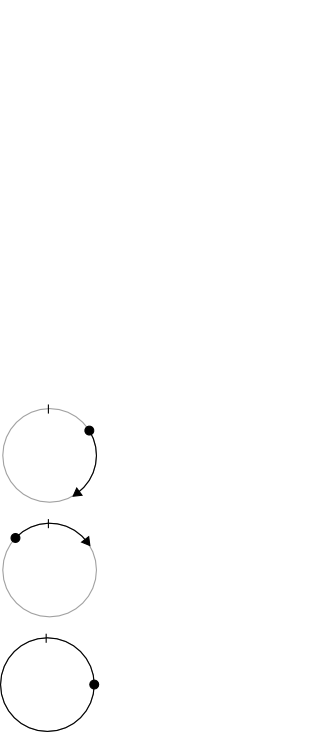
\includegraphics[width=0.2\linewidth]{figures/circular_intervals/cw.png}
\caption{The three kinds of clockwise intervals.}
\end{marginfigure}
$$cw_n(i,j) = 
\begin{cases}
\{k \in \ZZ \mid i < k < j\} & i < j \\
\{k \in \ZZ \mid 0 \le k < j \mbox{ or } i < k < n \} & i > j \\
\{k \in \ZZ \mid 0\le k < n, k\ne i \} & i = j\\
\end{cases}.$$
These are the indices in between $i$ and $j$ on the curve, where we
move ``clockwise'' in the direction of increasing indices.  We also
introduce counter-clockwise intervals
\begin{marginfigure}
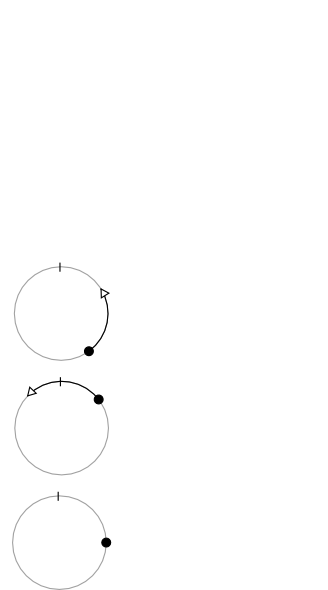
\includegraphics[width=0.2\linewidth]{figures/circular_intervals/ccw.png}
\caption{The three kinds of counter-clockwise intervals.}
\end{marginfigure}
$$ccw_n(i,j) = 
\begin{cases}
\{k \in \ZZ \mid 0 \le k < i \mbox{ or } j < k < n \} & i < j \\
\{k \in \ZZ \mid j < k < i\} & i > j \\
\emptyset & i = j\\
\end{cases}.$$
These are the points which are outside of the clockwise interval
between $i$ and $j$, excluding $i$ and $j$.

We can then adapt Observations \ref{obs-inside-rec} and \ref{obs-outside-rec} as follows:

\begin{prop}
We can recursively compute inside weights in time $O(|\RRR| n^3)$:

\begin{align*}
CInside_\GGG^C(X_{i i+1}) &= P_{sub} (\langle X_{ii+1} \to \ell_{i i+1}\rangle) \\
CInside_\GGG^C(X_{(n-1)0}) &= P_{sub} (\langle X_{(n-1)0} \to \ell_{(n-1)0}\rangle) \\
CInside_\GGG^C(X_{ij}) &= \sum_{\substack{[X\to YZ]\in \RRR(X)\\ k\in cw_n(i,j)}} 
P_{sub}(\langle X_{ij} \to Y_{ik} Z_{kj}\rangle) CInside_\GGG^C(Y_{ik}) CInside_\GGG^C(Z_{kj}).
\end{align*}
\end{prop}

\begin{prop}
We can recursively compute outside weights in time $O(|\RRR| n^3)$:

\begin{align*}
COutside_\GGG^C(S_{ii}) &= 1\\
COutside_\GGG^C(X_{ij}) &=
\sum_{\substack{h\in ccw_n(i,j) \\ [Z\to YX] \in \RRR}} P_{sub}(\langle Z_{hj} \to Y_{hi} X_{ij} \rangle)
COutside_\GGG^C(Z_{hj}) CInside_\GGG^C(Y_{hi})\\
&+ \sum_{\substack{k \in ccw_n(i,j)\\ [Z\to XY] in \RRR}}
P_{sub}(\langle Z_{ik} \to X_{ij} Y_{jk} \rangle)
COutside_\GGG^C(Z_{ik}) CInside_\GGG^C(Y_{jk}).
\end{align*}
\end{prop}

%% \subsubsection{old stuff about closed curves}

%% The probability that we see a parse tree is therefore $P(C,T\mid \GGG)
%% = \frac{1}{n} W_\GGG(T).$ The inside weights are unaffected by this
%% change - once we specify the root node $X_{ij}$, it is irrelevant
%% which shift of $C$ is being examined. (Although some shifts will not
%% allow $X_{ij}$, since $C[j]$ will be to the left of $C[i]$.)

%% The outside weights are affected by the change. For each $k$ such that
%% $0\le k < n$, we have a distinct $Outside_\GGG^{C^{\leftarrow
%%     k}}(X_{ij})$.
%% We can simplify matters by defining 
%% $$COutside_\GGG^C(X_{ij}) = \frac{1}{n} \sum_k
%% Outside_\GGG^{C^{\leftarrow k}}(X_{(i + k \mod n) (j + k \mod n)}).$$

%% \begin{prop}
%% We can compute $COutside_\GGG^C(X_{ij})$ recursively as follows:
%% $$COutside_\GGG^C(S_{ii}) = \frac{1}{n}.$$

%% \begin{align*}
%% COutside_\GGG^C(X_{ij}) &=
%%    \sum_{\substack{h < i \\ [Z\to YX] \in
%%     \RRR}} P_{sub}(\langle Z_{hi} \to Y_{hi}X_{ij} \rangle)
%% COutside_\GGG^C(Z_{hj}) Inside_\GGG^C(Y_{hi})\\
%% &+
%%  \sum_{\substack{j<k \\ [Z\to XY] \in
%%     \RRR}} P_{sub}(\langle Z_{ik} \to X_{ij}Y_{jk} \rangle)
%% COutside_\GGG^C(Z_{ik}) Inside_\GGG^C(Y_{jk})
%% \end{align*}
%% \end{prop}
%% \begin{proof}
%% \mar{finish and prove by induction.}
%% We proceed by downwards induction on the length of $X_{ij}$. The value
%% for $COutside_\GGG(S_{ii})$ is straight from the definition.

%% \end{proof}

\marginnote{end of parsing\_em.tex}

    \marginnote{Beginning of learning/doing\_em.tex}

\section{EM}
\marginnote{We want pictures of a grammar that does visible learning
  in a single iteration. The simplified hand is a nice
  example. Perturb the midpoint distributions and then try to recover
  them by retraining.}

\marginnote{Pictures to represent what EM does generically? Not clear
  how much insight it provides.}

Let $C_1,\dots, C_n$ be independent samples from a grammar $\GGG$, for
which we know the structure, but not the parameters. We would like to
set the parameters of $\GGG$ such that the posterior $P(\GGG\mid
C_1,\dots,C_n)$ is maximized. We can write the posterior as
\begin{align*}
  P(\GGG\mid C_1,\dots, C_n) &= P(\GGG) \cdot \frac{\prod_i P(C_i\mid \GGG)}{\prod_i P(C_i)}\\
  &\propto P(\GGG) \cdot \prod_i \sum_{T\in Parse_\GGG(C_i)}P(C_i, T \mid \GGG)\\
  &= P(\GGG) \cdot \sum_{\{T_i\}}\prod_i P(C_i, T_i \mid \GGG)\\
\end{align*}
Unfortunately, it is not known how to maximize this posterior, or even
the likelihood. The likelihood is known to have many local maxima in
the case of context-free grammars for natural languages
\cite{charniak}. Therefore, we are forced to use approximation
techniques. We use the Expectation-Maximization algorithm \cite{em},
which is a standard approach to finding maximum likelihood or maximum
a posteriori estimates in the case where important variables are
unobserved. In our case, the unobserved variables are the parse trees
$\{T_i\}$.

Let $\mathbf{C} = (C_1,\dots,C_n)$, and let $\mathbf{T}$ be the latent
variable $(T_1,\dots,T_n)$. We then iteratively find better and better
grammars $\GGG^{(t)}$:
\begin{enumerate}
\item \textbf{E step:} Let 
  \begin{align*}
Q^{(t)}(\GGG) &= \sum_{\mathbf{T}} \big[P(\mathbf{T}\mid \mathbf{C},
\GGG^{(t)}) \log P(\mathbf{C},\mathbf{T}\mid \GGG) \big] + \log
P(\GGG)\\
&= E_{\mathbf{T} \sim \mathbf{T} | \mathbf{C}, \GGG^{(t)}}\big[\log
P(\mathbf{C},\mathbf{T}\mid \GGG) \big] + \log P(\GGG)
  \end{align*}
\item \textbf{M step:} Let
$$ \GGG^{(t+1)} = \argmax_{\GGG} Q^{(t)}(\GGG)$$
\end{enumerate}

\subsection{The E Step}

$$Q^{(t)}(\GGG) = E_{\mathbf{T}\sim \mathbf{T}, \GGG^{(t)}} [\log
P(C,T\mid \GGG)] + \log P(\GGG)$$
Since $P(\mathbf{C},\mathbf{T}\mid \GGG) = \prod_a P(C_a, T_a\mid \GGG),$
and by linearity of expectation:
$$Q^{(t)}(\GGG) = \sum_a E_{T_a\sim \Delta^{(t)}_a} [\log
P(C_a,T_a \mid \GGG)] + \log P(\GGG),$$
where $\Delta^{(t)}_a(T_a)$ is the distribution $P(T_a\mid C_a,
\GGG^{(t)})$.

Let $Q_a^{(t)}(\GGG) =E_{T_a \sim \Delta_a^{(t)}}[\log P(C_a,T_a\mid
\GGG)].$ We can decompose $P(C_a, T_a\mid \GGG)$ by using Proposition
\ref{prop-inside-corr} \footnote{If $\GGG$ is a grammar for closed curves,
  $P(C_a,T_a\mid \GGG)$ will have an extra factor of
  $\frac{1}{|C|}$. We can ignore this because the logarithm turns it
  into an additive constant, which is irrelevant in the M step.}:

\begin{align*}
  Q_a^{(t)}(\GGG) &=
E_{T_a \sim \Delta_a^{(t)}}\left[\log
    \prod_{\langle X_{ij} \to \lambda\rangle \in T_a} P_{sub}(\langle
    X_{ij} \to \lambda\rangle)\right]\\
&=
E_{T_a \sim \Delta_a^{(t)}}\left[
    \sum_{\langle X_{ij} \to \lambda\rangle \in T_a} \log P_{sub}(\langle
    X_{ij} \to \lambda\rangle)\right]\\
\intertext{
We can rewrite this as a sum over all possible concrete
  substitution rules, using indicator variables to eliminate absent terms:}
&=
E_{T_a \sim \Delta_a^{(t)}}\Bigg[
\sum_{i < j < k} \sum_{[X\to YZ]\in \RRR}\ind [ 
\langle X_{ik}
\to Y_{ij} Z_{jk} \rangle] \quad \log P_{sub}(\langle X_{ik} \to Y_{ij}
Z_{jk}\rangle )\\
&\qquad+\qquad \sum_{i} \sum_{[X\to \ell]\in \RRR}\ind [ \langle X_{i i+1}
\to \ell_{i i+1} \rangle] \quad \log P_{sub}(\langle X_{i i+1} \to \ell_{i i+1}\rangle)
\Bigg]\\
&=
\sum_{i < j < k} \sum_{[X\to YZ]\in \RRR} \log P_{sub}(\langle X_{ik} \to Y_{ij}
Z_{jk}\rangle ) \quad E_{T_a \sim \Delta_a^{(t)}}[\ind [ 
\langle X_{ik}
\to Y_{ij} Z_{jk} \rangle]]\\
&+ \sum_{i} \sum_{[X\to \ell]\in \RRR}
\log P_{sub}(\langle X_{i i+1} \to \ell_{i i+1}\rangle)
\quad E_{T_a \sim \Delta_a^{(t)}}[\ind [ \langle X_{i i+1}
\to \ell_{i i+1} \rangle]] 
\end{align*}
In the case of closed curves, the sum over $i < j < k$ will instead be
over $0\le i,k \le n$, and $j\in cw_n(i,k)$.

\marginnote{Pick a particular rule $X\to YZ$ and show the heaviest few
  values over $a,i,j,k$. This should give a lot of insight into the
  soft counts.}

Let 
\begin{align*}
  Count_a^{(t)}(\langle X_{ik} \to Y_{ij} Z_{jk} \rangle) &=  E_{T_a \sim \Delta_a^{(t)}}[\ind [ 
\langle X_{ik}
\to Y_{ij} Z_{jk} \rangle]]\\
&= P_{T_a \sim \Delta_a^{(t)}}( \langle X_{ik} \to Y_{ij} Z_{jk}
\rangle \in T_a)\\
Count_a^{(t)}(\langle X_{ii+1} \to \ell_{i i+1} \rangle) &=
E_{T_a \sim \Delta_a^{(t)}}[\ind [ \langle X_{i i+1}
\to \ell_{i i+1} \rangle]] \\
&= P_{T_a \sim \Delta_a^{(t)}}( \langle X_{i i+1} \to \ell_{i i+1} \rangle \in T_a)\\
\end{align*}
and let
\begin{align*}
  Q^{(t)}_{a,i,j,k,[X\to YZ]}(\GGG) &= 
\log P_{sub}(\langle X_{ik} \to Y_{ij}
Z_{jk}\rangle ) \cdot   Count_a^{(t)}(\langle X_{ik} \to Y_{ij} Z_{jk} \rangle)\\
Q^{(t)}_{a,i,[X\to \ell]}(\GGG) &=
\log P_{sub}(\langle X_{i i+1} \to \ell_{i i+1}\rangle)
\cdot Count_a^{(t)}(\langle X_{ii+1} \to \ell_{i i+1} \rangle).
\end{align*}

\subsection{Computing the Soft Counts}
In this section, we show how to compute the soft counts from the inside and outside weights.

Firstly,
\begin{align*}
\Delta_a^{(t)} &= P(T_a \mid C_a, \GGG^{(t)})\\
 &= \frac{P(C_a, T_a \mid \GGG^{(t)})}{P(C_a \mid \GGG^{(t)})}\\
&= \frac{P(T_a \mid \GGG^{(t)})}{P(C_a \mid \GGG^{(t)})}.\\
\end{align*}

\begin{defn}
A {\em complete parse tree} is a parse tree with root node $S_{0n}$,
and which has no unexpanded nodes. We will denote the set of complete
$\GGG$-parse trees of $C$ by $\FF_\GGG^C$. We will denote the set of
complete $\GGG$-parse trees of $C$ which contain a node $\langle
X_{ij}\to \lambda \rangle$ by $\FF_\GGG^C(X_{ij}, \lambda)$.
\end{defn}

\begin{prop}
Every parse tree $T \in \FF_\GGG^C(X_{ij}, \lambda)$ can be obtained as
$$T_{out} \triangle^{\cancel{X_{ij}}}_{(X_{ij},\lambda)} T_{in},$$ 
where $T_{out}\in \Outer_\GGG^C(X_{ij})$ and $T_{in} \in
\Inner_\GGG^C(X_{ij}, \lambda)$.
\end{prop}
\begin{proof}
If we remove the subtree rooted at the node $\langle X_{ij} \to
\lambda \rangle$ and replace it with an unexpanded node $X_{ij}$, the
resulting tree is an outer parse tree in $\Outer_\GGG^C(X_{ij})$. The
subtree rooted at $\langle X_{ij} \to \lambda\rangle$ is an inner
parse tree with root $\langle X_{ij} \to \lambda \rangle$.
\end{proof}

\begin{obs}
For open curves $C$,
\begin{align*}
P(\langle X_{ij} \to \lambda \rangle \in T \mid \GGG) &=
\sum_{T \in \FF_\GGG^C(X_{ij}, \lambda)} W_\GGG(T)\\
\intertext{which, by the previous proposition can be broken up as}
&=
\left(\sum_{T_{out}\in \Outer_\GGG^C(X_{ij})}
  W_\GGG(T_{out}) \right)
\left(\sum_{T_{in}\in \Inner_\GGG^C(X_{ij},\lambda)} W_\GGG(T_{in})
\right)\\
&= Outside_\GGG^C(X_{ij}) Inside_\GGG^C(X_{ij}, \lambda).
\end{align*}
For closed curves $C$, 
\begin{align*}
P(\langle X_{ij} \to \lambda \rangle \in T \mid \GGG) &=
\frac{1}{|C|} \sum_{T \in \FF_\GGG^C(X_{ij}, \lambda)} W_\GGG(T)\\
&= \frac{1}{|C|} COutside_\GGG^C(X_{ij}) CInside_\GGG^C(X_{ij}, \lambda).
\end{align*}

\end{obs}

In particular, for open curves, $P(C \mid\GGG) = Inside_{\GGG}^{C}(S_{0n})$, and for closed curves, 
$P(C\mid \GGG) = \frac{1}{|C|} \sum_{i=0}^{n-1} CInside_\GGG^C(S_{ii})$.
Thus, for open curves,
$$Count_a(\langle X_{ij} \to \lambda \rangle) = 
\frac{Outside_{\GGG^{(t)}}^{C_a}(X_{ij}) Inside_{\GGG^{(t)}}^{C_a}(X_{ij},\lambda)}{
Inside_{\GGG^{(t)}}^{C_a}(S_{0n})}, $$
and for closed curves,
$$Count_a(\langle X_{ij} \to \lambda \rangle) = 
\frac{COutside_{\GGG^{(t)}}^{C_a}(X_{ij}) CInside_{\GGG^{(t)}}^{C_a}(X_{ij},\lambda)}{
\frac{1}{|C_a|} \sum_{i=0}^{n-1} CInside_{\GGG^{(t)}}^{C_a}(S_{ii})}, $$

To summarize,

\begin{centering}
\framebox{
\parbox{5in}{
\begin{align*}
  Q^{(t)}(\GGG) &= \sum_a \sum_{i,j,k} \sum_{[X\to YZ]\in \RRR}
  Q^{(t)}_{a,i,j,k,[X\to YZ]}(\GGG)\\
&+ \sum_a \sum_{i} \sum_{[X\to \ell]\in \RRR}
  Q^{(t)}_{a,i,[X\to \ell]}(\GGG)\\
&+ \log P(\GGG)
\end{align*}

\begin{align*}
  Q^{(t)}_{a,i,j,k,[X\to YZ]}(\GGG) &= 
\log P_{sub}(\langle X_{ik} \to Y_{ij}
Z_{jk}\rangle ) \cdot   Count_a^{(t)}(\langle X_{ik} \to Y_{ij} Z_{jk} \rangle)\\
Q^{(t)}_{a,i,[X\to \ell]}(\GGG) &=
\log P_{sub}(\langle X_{i i+1} \to \ell_{i i+1}\rangle)
\cdot Count_a^{(t)}(\langle X_{ii+1} \to \ell_{i i+1} \rangle) \\
\end{align*}

\begin{align*}
Count_a(\langle X_{ij} \to \lambda \rangle) &= 
\frac{Outside_{\GGG^{(t)}}^{C_a}(X_{ij}) Inside_{\GGG^{(t)}}^{C_a}(X_{ij},\lambda)}{
Inside_{\GGG^{(t)}}^{C_a}(S_{0n})}, 
\intertext{for open curves, and}
Count_a(\langle X_{ij} \to \lambda \rangle) &= 
\frac{COutside_{\GGG^{(t)}}^{C_a}(X_{ij}) CInside_{\GGG^{(t)}}^{C_a}(X_{ij},\lambda)}{
\frac{1}{|C_a|} \sum_{i=0}^{n-1} CInside_{\GGG^{(t)}}^{C_a}(S_{ii})}, 
\intertext{for closed curves.}
\end{align*}
}
}
\end{centering}

\marginnote{End of learning/doing\_em.tex}


    \marginnote{Merge the following with the previous. The subsection
      ``Scale-dependent Dirichlet Prior'' should have much of its
      material moved to the Models chapter, since it is largely about
      selecting an initially plausible set of parameters.}

    % parameters.tex

\marginnote{beginning of learning/parameters.tex}

In order to learn a shape grammar $\GGG =
(\NNN,\RRR,\SSS,\ell,\MMM,\XXX)$, we must learn (1) the structural
elements of the grammar ($\NNN, \RRR, \SSS$); (2) the continuous
elements of the grammar (the multinomial distributions $\XXX$), and
(3) the associated geometric information (the midpoint distributions
$\MMM$). Learning the structural elements of the grammar is a very
difficult unsolved problem, and we defer the topic to Section
\ref{sec-learn-struct}.

For the multinomial distributions and the midpoint distributions, we
use the Expectation-Maximization algorithm \cite{em}.  

\subsection{EM for Parameter Estimation}

Let $C_1,\dots, C_n$ be independent samples from a grammar $\GGG$, for
which we know the structure, but not the parameters. We would like to
set the parameters of $\GGG$ such that the posterior $P(\GGG\mid
C_1,\dots,C_n)$ is maximized. We can write the posterior as
\begin{align*}
  P(\GGG\mid C_1,\dots, C_n) &= P(\GGG) \cdot \prod_i P(C_i\mid \GGG)\\
  &= P(\GGG) \cdot \prod_i \sum_{T\in Parse_\GGG(C_i)}P(C_i, T \mid \GGG)\\
  &= P(\GGG) \cdot \sum_{\{T_i\}}\prod_i P(C_i, T_i \mid \GGG)\\
\end{align*}
Unfortunately, it is not known how to maximize this posterior, or even
the likelihood. The likelihood is known to have many local maxima in
the case of context-free grammars for natural languages
\cite{charniak}. Therefore, we are forced to use approximation
techniques. We use the Expectation-Maximization algorithm \cite{em},
which is a standard approach to finding maximum likelihood or maximum
a posteriori estimates in the case where important variables are
unobserved. In our case, the unobserved variables are the parse trees
$\{T_i\}$.

Let $\mathbf{C} = (C_1,\dots,C_n)$, and let $\mathbf{T}$ be the latent
variable $(T_1,\dots,T_n)$. We then iteratively find better and better
grammars $\GGG^{(t)}$:
\begin{enumerate}
\item \textbf{E step:} Let 
  \begin{align*}
Q^{(t)}(\GGG) &= \sum_{\mathbf{T}} \big[P(\mathbf{T}\mid \mathbf{C},
\GGG^{(t)}) \log P(\mathbf{C},\mathbf{T}\mid \GGG) \big] + \log
P(\GGG)\\
&= E_{\mathbf{T} \sim \mathbf{T} | \mathbf{C}, \GGG^{(t)}}\big[\log
P(\mathbf{C},\mathbf{T}\mid \GGG) \big] + \log P(\GGG)
  \end{align*}
\item \textbf{M step:} Let
$$ \GGG^{(t+1)} = \argmax_{\GGG} Q^{(t)}(\GGG)$$
\end{enumerate}

We compute only what is necessary to optimize $Q^{(t)}(\GGG)$. The
joint log-likelihood can be calculated as follows:
\begin{align*}
  P(\mathbf{C},\mathbf{T}\mid \GGG) = &\prod_a \prod_{(X,[X\to YZ],i,j,k)\in T_a} \rho_X([X\to YZ]) \cdot \mu_{X\to YZ}(C_a[i], C_a[j], C_a[k]) \\
  \cdot &\prod_a \prod_{(X,[X\to \ell],i,\bot,j)\in T_a} \rho_X([X\to \ell]) \\
  \log P(C,T\mid \GGG) = &\sum_a \sum_{[X\to \lambda] \in \RRR}
  \#\{\mbox{uses of }[X\to \lambda]\mbox{ in } T_a \} \log \rho_X([X\to \lambda]) +\\
  &\sum_a \sum_{[X\to YZ] \in \RRR} \sum_{(X, [X\to YZ], i, j,k)\in T_a} \log
  \mu_{X\to YZ}(C_a[i], C_a[j], C_a[k])\\
\end{align*}

We wish to optimize $Q^{(t)}$ with respect to the multinomial
distributions $\rho_X$ for each $X$. The joint likelihood given in
Equation \ref{joint-likelihood} depends on the $\rho_X$ only as $\prod
\rho_X()$. Taking logs, and by the linearity of expectation, the
relevant part of $Q^{(t)}$ is
$$\sum_a \sum_\lambda E_{T_a}\left[ \#\left\{\mbox{uses of }[X\to
    \lambda] \mbox{ in }T_a \right\}\right]\cdot \log \rho_{X}([X\to \lambda]) +
\log P(\rho_X).$$

This has the same form as the log-posterior of a multinomial
distribution under the Dirichlet prior, as we will see in Section
\ref{sec-multinomial}. The observed multinomial counts are a
sufficient statistic, so we need only compute $\sum_a E_{T_a}\left[
  \#\left\{\mbox{uses of }[X\to \lambda] \mbox{ in } T_a
  \right\}\right]$ for each $\lambda$. We call this quantity a
\emph{soft count}.

Similarly, we wish to optimize $Q^{(t)}$ with respect to the midpoint
distributions $\mu_{X\to YZ}$; however, we are using a nonparametric
midpoint distribution, so this question is ill-posed. We adapt the
Parzen window density estimator by using the soft counts instead of
multiplicities. The formula for this is given in Section
\ref{sec-learn-midpoint}.  The formula for the soft counts is:
$$\sum_a \sum_{0\le i < j < k\le n} \log \mu_{X\to YZ}(C_a[i], C_a[j], C_a[k])
 E_{T_a}\left[ \xi_{a, X\to YZ, i,j,k} \right],$$
where we define
$$\xi_{a, X\to YZ,i,j,k}$$
to be one if the parse tree $T_a$ uses $X\to YZ$ to parse the curve
$C_a[i:k]$, divided into $C_a[i:j]$ and $C_a[j:k]$, and zero otherwise.

We have thus reduced the problem of learning parameters to the problem
of finding the soft counts. How do we find the soft counts?  We need
to compute $E_{T_a} \xi_{a,X\to YZ,i,j,k}$ for every $a$, $[X\to YZ],
i,j,k$. Since $\xi_{a, X\to YZ,i,j,k}$ is an indicator variable, this
is the same as computing the total probability that the rule $[X\to
YZ]$ appears in the specified location, which can be obtained by
summing Equation \eqref{joint-likelihood} over all parse trees that
use $[X\to YZ]$ in the specified location.

This probability can be calculated efficiently using the
Inside-Outside algorithm, which can be derived from the equations in
Section \ref{sec-parsing}. The inside probability is given in the
second-to-last equation of Section \ref{sec-parsing}. We do not give
the equations for the outside probability, but they are derived in a
similar way.

The soft counts $E_{T_a}\left[ \#\left\{\mbox{uses of
    }[X\to \lambda] \mbox{ in } T_a\right\}\right]$ can be found by summing the
relevant $\xi$.

\subsection{Learning Multinomial Distributions}
\label{sec-multinomial}

A multinomial distribution is a distribution over a finite alphabet
$a_1,\dots, a_k$, where $P(a_i)=p_i$. Learning a multinomial
distribution from independent samples $x_1,\dots, x_n$ is commonly done by
maximizing the posterior probability 
\begin{align*}
\vec{p} = (\widehat{p_1},\dots, \widehat{p_k}) &= \argmax_{\vec{p}}
P(\vec{p} \mid x_1,\dots,x_n )\\
&= \argmax_{\vec{p}} P(x_1,\dots,x_n; \vec{p}) \cdot P(\vec{p}),
\end{align*}
where $P(\vec{p})$ is a prior distribution over the space of possible
$(p_1,\dots,p_k)$. The most common choice of prior is the Dirichlet
distribution, parameterized by $\alpha_1,\dots, \alpha_k > 0$:
$$\mathrm{Dir}(p_1,\dots, p_k; \alpha_1,\dots, \alpha_k) = \frac{\Gamma\bigl(\sum \alpha_i\bigr)}{\prod \Gamma(\alpha_i)} \prod_{i=1}^k p_i^{\alpha_i - 1},$$
because, when all $\alpha_i \ge 1$, the maximum a posteriori estimate of the $\{p_i\}$ has the simple form
$$\widehat{p_i} = \frac{ c_i + \alpha_i - 1}{ n + \sum
  \alpha_i - k},$$ 
where
$$c_i = \#\{j : x_j = i\}.$$
More generally, the maximum a posteriori estimate has the form
$$\widehat{p_i} = \begin{cases}
\frac{ c_i + \alpha_i - 1}{ n + \sum_{i\in I} \alpha_i - |I|} & c_i + \alpha_i \ge 1\\
0 & \mbox{ otherwise}\\
\end{cases},$$ 
where
$$I = \{i : c_i + \alpha_i \ge 1\}.$$

When the $\alpha_i$ are greater than one, this prior smooths the
estimated distribution $\vec{p}$ towards the uniform
distribution. When the $\alpha_i$ are less than one, this prior makes
the distribution sparser than the maximum likelihood estimate. 

When estimating the production probabilities in a grammar, a
sparsifying prior is generally recommended. One intuition for this is
that we are trying to recover a relatively sparse set of rules from
the set of all possible rules; in order to avoid missing a rule, we
must give some weight to (and thus generate observations of) rules
that will ultimately be discarded. In \cite{johnson-naacl}, a
Dirichlet prior with $\alpha_i = \frac{1}{1000}$ was found to work
well for training context-free grammars for natural languages,
although $\alpha_i$ between $\frac{1}{100}$ and $\frac{1}{10,000}$
were found to work about as well.

\subsection{Scale-dependent Dirichlet Prior}
\label{sec-scale}

When there is no prior reason to believe that any $p_i$ is larger than
the others, it is natural to use a Dirichlet prior with each
$\alpha_i$ the same. For shape grammars, this is not entirely the
case; since rules of the form $[X\to YZ]$ and $[X\to \ell]$ serve
different roles in the grammar, we expect their probabilities to take
on different values. 

In particular, if the nonterminal $X$ is meant to model long curves,
it is unlikely that a long curve will have only two sample points,
especially if we are parsing a curve that has many sample
points. Therefore, we would expect the probability of $[X\to \ell]$ to
be low.

Let $C$ be a curve. We define the \emph{scale} of a subcurve $C'$ to
be $s(C') = |C'| / |C|$. We can then specify an ideal scale $s_X$ for
the nonterminal $X$. Our prior distribution on $\rho_X$ is then
$Dir(\alpha_1,\dots,\alpha_k)$, where
\begin{align*}
\alpha_1 &= k \cdot \alpha_{dir} \cdot e^{-\omega s_X^2}k &\\
\alpha_i &= k \cdot \alpha_{dir} \cdot \frac{1 - e^{-\omega s_X^2}}{k-1} & 2 \le i \le k.\\
\end{align*}
Here $\alpha_1$ corresponds to the rule $[X\to \ell]$. Suitable values
of $\alpha_{dir}$ are probably significantly less than one, in light
of \cite{johnson-naacl}. A suitable value for $\omega$ is more
complicated, and depends on the value of other model parameters.

This prior is suitable, because it produces grammars biased towards
balanced parses. To see this, consider a grammar $\GGG$ whose
parameters are set according to this prior. (This will be true of our
initial grammar, as we describe in Section \ref{sec-single}.)  Let $C$ be a
curve of length $n$, and $T$ be a $\GGG$-parse of $C$. $T$ will then
specify nonterminals $X_1,\dots,X_n$ to parse each line segment of
$C$. Thus, the likelihood $P(C,T\mid \GGG)$ will contain factors
$\rho_{X_i}([X_i\to \ell])$ for $i=1,\dots,n$. If $\rho_{X_i}([X_i\to
\ell])$ is $e^{-\omega s_X^2}$, then these factors contribute
$$e^{-\omega \sum_i s_{X_i}^2}$$
in total. Since the $X_i$ combine to parse $C$, the scales $s_{X_i}$
will hopefully sum to approximately one. In this case the probability
will be highest when $\sum_i s_{X_i}^2$ is lowest, which occurs when
all the $s_{X_i}$ are equal. The stated Dirichlet prior thus pushes
$\GGG$ to favor balanced parse trees, as desired.

\marginnote{Would it make sense to do experiments trying to learn
  $P(X\to \ell)$?}

\marginnote{end of learning/parameters.tex}


  \section{Practical Use of the EM Algorithm with Curve Grammars:
    Obstacles and Strategies}
    
\subsection{Simple tuning}

Here is our example curve, from which we build a grammar with hand-chosen rules.

\includegraphics[width=2in]{./3.em/simple_tuning/examples.eps}

Here are our training curves:
\includegraphics[width=2in]{./3.em/simple_tuning/training.eps}

Here is the grammar:

\subsubsection{Initial}
Here are some samples from the grammar:

\includegraphics[width=6in]{output/3.learning/incremental/gram.19.d/samples.png}



\subsubsection{Round 1}
Here are some samples from the grammar:

\includegraphics[width=6in]{output/3.learning/incremental/gram.19.d/samples.png}


\subsubsection{Round 2}
Here are some samples from the grammar:

\includegraphics[width=6in]{output/3.learning/incremental/gram.19.d/samples.png}


\subsubsection{Round 3}
Here are some samples from the grammar:

\includegraphics[width=6in]{output/3.learning/incremental/gram.19.d/samples.png}


\subsubsection{Round 4}
Here are some samples from the grammar:

\includegraphics[width=6in]{output/3.learning/incremental/gram.19.d/samples.png}


\subsubsection{Round 5}
Here are some samples from the grammar:

\includegraphics[width=6in]{output/3.learning/incremental/gram.19.d/samples.png}



    
\FloatBarrier

\section{Tuning with multiple midpoints, and curves of constant length}

\marginnote{?}
There may be a small bug here, since EM should settle into a local
optimum, and the algorithm seems to be cycling between two relatively
reasonable grammars. Presumably has to do with the sparsifying
manipulations of the soft counts.

Here is our example curve, from which we build a grammar with
hand-chosen rules. We then enrich the grammar by adding in several
copies of each rule, with jittered midpoints.

\begin{figure}
\includegraphics[width=0.5\linewidth]{experiments/3.em/multi_tuning/output.d/examples.png}
\caption{
Here is our example curve, from which we build a grammar
with hand-chosen rules. We then enrich the grammar by adding in
several copies of each rule, with jittered midpoints
}
\end{figure}

\marginnote{?}
Here are our training curves. We have removed one of the curves from
the training set because its correspondence to the original curve is
questionable. (It is from a frame during the flipping around of the
arm, and it is hard to pick a labeling of the points that is
consistent throughout that transition.)

\begin{figure}
\includegraphics[width=0.5\linewidth]{experiments/3.em/multi_tuning/output.d/training.png}
\caption{Here are our training curves:}
\end{figure}

Round 10:

Here are some samples from the grammar:

\includegraphics[width=6in]{output/3.learning/incremental/gram.19.d/samples.png}




    
\FloatBarrier

\section{Tuning with multiple midpoints, learning multi-level correlations}

Here is the training data:

\begin{figure}
\includegraphics[width=3in]{experiments/3.em/correlated_tuning/output.d/training.png}
\end{figure}

Round 10:

Here are some samples from the grammar:

\includegraphics[width=6in]{output/3.learning/incremental/gram.19.d/samples.png}




    \input{experiments/3.em/sdf_tuning/sdf_tuning}
    \documentclass{article}
\usepackage{leonine,amsmath,amssymb,amsthm,graphicx, setspace}%%xy, setspace, amscd (commutative diagram)
\title{Notes}

\author{Eric Purdy \footnote{Department of Computer Science,
    University of Chicago. Email: epurdy@uchicago.edu}}

%%\doublespace
\DeclareMathOperator*{\len}{len}
\newcommand\fakecite[1]{ {\bf [#1]} }

%% \newcommand\spk[2]{\includegraphics[width=#1mm]{images/#2.png}}
\newcommand\spk[2]{\framebox{images/#2.png}}

\begin{document}
\maketitle

\tableofcontents

\part{CURRENT WORK}

\section{Style Guide}

This is just a convenient reference for me as I try to keep all the
notation consistent and intuitive.

\bitem
\item Nonterminals: $X,Y,Z$ (use superscripts to enumerate)
\item Placed nonterminals: $X_{p,q}$
\item Start nonterminals: $S,T$
\item Terminal: $\ell$
\item Placed terminal: $\ell_{p,q}$
\item Curves: $A,B,C, C_n$
\item Points: $c_i$
\item Curvilinear forms: $\lambda, \mu, \nu$ ($\sigma$ for starting)
\item Grammars: $\GGG, \HHH$
\item Set of nonterminals: $\NNN$
\item Set of starting nonterminals: $\SSS$
\item Set of rules: $\RRR, \RRR(X)$
\item Set of midpoint distributions: $\MMM$
\item Set of rule-choice distributions: $\XXX$.
\item Do we want to differentiate open/closed curves notationally?
$ST$ vs. $\overline{ST}$ is reasonable, if so.
\eitem

\section{Grammatical Curve Models }

Pedro's hierarchical curve models for curve classification

\subsection{The Task}

We want to build a system that can classify curves. We will give it a
set of curves from $n$ different classes $C_1,\dots,C_n$, and we wish
to assign new curves to the class that they most belong in. Some
datasets for this task are:
\bitem
\item Swedish Leaf dataset. Here we are given the silhouettes of
  leaves from fifteen different species of tree. (Species include
  maple, oak, and some sort of willow.) For each class, we are given
  25 example leaves, and then we want to build a classifier that will
  accurately classify another 50 examples from each species.

\item MPEG7.

\eitem

Our generic approach to this task will be to build a probabilistic
model for each class. Given a novel curve $x_*$, we will compute $\PP(
x_* \mid C_i)$ for each class and assign $x_*$ to the class which
gives it the highest likelihood.

\subsection{Some Motivation}

To motivate our discussion of curve grammars, we will first give an
amusing example of such a grammar, which is inspired by L-systems. A
Lindenmayer system, or L-system, is a parallel string rewriting
system. Although they are defined on strings, it is popular to render
their output as a picture using a ``turtle language'' akin to
Logo. They are a simple and intuitive way to generate fractal
images. Since our formalisms do not match up perfectly with the usual
definition of L-systems, we will not discuss them.

We will informally discuss curve rewriting systems, where we
iteratively replace straight lines with curves composed of straight
lines. We will represent our curves like this: \spk{10}{gline}, so that
we remember which endpoint is which.

Consider the following system\footnote{generated by $A=A+A+A--$ with
  angle $60^\circ$ in Inkscape}:
$$ \spk{10}{gline} \to \spk{10}{gbump} .$$

Applying this rule a few times, we generate \spk{10}{gline}, \spk{10}{gbump},
\spk{10}{gbump2} and \spk{15}{gbump3}.

%% An L-system might represent
%% this rewrite rule as $A\to A+A+A$. Here, if we interpret the symbol
%% $A$ as ``go forward one step'' and the symbol $+$ as ``rotate 60
%% degrees to the left'', then a turtle following the directions $A+A+A$
%% would generate the curve \includegraphics[width=10mm]{bump.png},
%% suitably rotated.

We now wish to construct a more complicated system. We need to start
distinguishing different kinds of curves, in this case \spk{10}{gdash}
versus \spk{10}{gline}. Consider the following system\footnote{generated by 
$A=B+A+B; B=A-B-A$ with angle $60^\circ$ in Inkscape}
\begin{align*}
\spk{15}{gline} &\to \spk{15}{gBAB} \\
\spk{15}{gdash} &\to \spk{15}{gABA}.
\end{align*}

If we start from \spk{10}{gline}, we successively generate
\spk{10}{gBAB}, \spk{20}{gsier2}, and \spk{20}{gsier3}.  Suprisingly,
after a large number of iterations, a pattern arises that may be
familiar: Sierpinski's triangle! After eight iterations, we have
(filling in the dashed lines for simplicity) curve $C$:

\spk{100}{gsier8}.

These curves were generated by Inkscape's L-system function, which has
a randomizing option. It is interesting to randomize the last
example. Here is the randomized version $C'$ I got, with fairly little
noise (10\% randomization in the length of line segments, and 5\%
randomization in the angles. These parameters only make sense in a
more standard L-system framework):

\spk{100}{gbadsier}.

This has no global similarity at all to the other curve! Inkscape is
using a Markov-like source of randomness, and little errors at the
local level add up to huge changes at the global level. If we are
going to have a statistical model for perceptual similarity of curves,
we will have to find a way to introduce long-range dependencies. This
brings us to our next section: probabilistic context-free grammars on
curves.

\subsection{Model: PCFG's on Curves}

Our probabilistic models will be probabilistic context-free grammars.
We define a Probabilistic Context-Free Grammar framework for
generating and parsing one-dimensional curves in a two-dimensional
space.

We will represent a curve as a sequence of oriented line segments. We
will denote a line segment going from points $p$ to point $q$ by
$\ell_{p,q}$. A curve will then have the form
$$ \ell_{p_0,p_1} \ell_{p_1,p_2}\cdots \ell_{p_{n-1},p_n},$$ and
$p_0$ will be equal to $p_n$ iff the curve is closed.  For a closed
curve, this sequence is circular, and we consider any cyclic
permutation of the line segments to be the same curve.

Analogously to context-free grammars over strings, we introduce
non-terminals. Our non-terminals will represent oriented curves
(either open or closed) whose endpoints are fixed, but whose path
between those endpoints is unspecified. We denote such a non-terminal
of type $N$ going from point $p$ to point $q$ by $N_{p,q}$. By itself,
$N$ will denote a type of non-terminal that can be instantiated
between any $p$ and $q$.

\begin{defn}
A {\em curvilinear form} (by analogy with a sentential form for string
grammars) is a sequence of oriented sub-curves denoted by
non-terminals. It will have the form
$$ \alpha^{(0)}_{p_0,p_1} \alpha^{(1)}_{p_1,p_2} \cdots
\alpha^{(n-1)}_{p_{n-1},{p_n}}$$ where each $\alpha^{(i)}$ can be
either $\ell$ or any non-terminal type. As with curves, $p_0$ will be
equal to $p_n$ iff the curvilinear form is closed.

We will also have {\em abstract curvilinear forms} which have no
associated geometric information. They will have the form
$$ \alpha^{(0)} \alpha^{(1)} \cdots \alpha^{(n-1)}.$$ We will specify
whether these are open or closed, since there is no way to
tell. Again, closed abstract curvilinear forms will be invariant under
cyclic permutations.
\end{defn}

We next introduce substitutions and substitution rules, which allow us
to transform curvilinear forms, ultimately producing curves. We will
perform substitutions of the form
$$ A_{p,q} \to B^{(1)}_{p,p_1} B^{(2)}_{p_2,p_3} \cdots
B^{(k)}_{p_k,q}.$$ Since $A_{p,q}$ represents an unspecified path from
$p$ to $q$, substitution simply gives a more specific route, in terms
of which points we will visit in between (the $p_i$, which we will
call ``control points'') and what sort of path we will follow between
these points (the $B^{(i)}$).

In order to give a substitution rule for performing substitutions, we
need to give
\bitem
\item An {\em abstract substitution rule} $A\to B^{(1)}\cdots B^{(k)}$.
\item a rule for determining the $p_i$ in terms of $p$ and $q$.
  \eitem

In order to make the rules be context-free, we would like the specific
path followed by $A_{p,q}$ (i.e., the $p_i$) to be independent of the
context in which $A_{p,q}$ occurs (i.e., $p$ and $q$), given that we
are taking this particular path. Accordingly, we specify the $p_i$ in
the coordinate system $\CCC(p,q)$ that maps $(0,0)$ to $p$ and $(1,0)$
to $q$.

In practice, applying a substitution rule is problematic because the
$p_i$ live in an infinite domain ($\RR^2$), but we want to deal with
curves that (1) live in a finite domain (the pixels of the image
plane) and (2) are expected to exhibit a good deal of variation. Thus,
we give a distribution over the $p_i$ called the control-point
distribution:
$$ \PP \left[ p_1,\dots, p_k \mid p,q \right] = \mu_{A\to
  B^{(1)}\cdots B^{(k)}}(p_1,\dots, p_k ; p,q).$$ Because we want a
context-free formulation, we will restrict the control-point
distribution to be of the form
$$ \PP \left[ p_1,\dots, p_k \mid p,q \right] = \mu_{A\to
  B^{(1)}\cdots B^{(k)}}( \widehat{p}_1, \dots, \widehat{p}_k)$$ where
$\widehat{p_i}$ are the coordinates of $p_i$ in $\CCC(p,q)$.

\begin{defn}
A probabilistic context-free shape grammar (PCFSG) is a tuple 
$\GGG = (\NNN, \RRR, \SSS, \ell, \MMM, \XXX)$, where
\bitem
\item $\NNN$ is a set of curve types
\item $\RRR$ is a set of abstract substitution rules
\item $\SSS$ is a set of starting curvilinear forms
\item $\ell \in \NNN$ is a curve type representing a line segment
\item $\XXX = \{\rho_X \mid X\in \NNN, X\ne \ell\} \cup
  \{\rho_\SSS\}$, where $\rho_X$ is a probability distribution over
  $\RRR(X)$, and $\rho_\SSS$ is a distribution over $\SSS$
\item $\MMM = \{ \mu_{X\to Y^{(1)}\cdots Y^{(k)}} \mid (X\to
  T^{(1)}\cdots Y^{(k)}) \in \RRR\}$ is a set of control-point
  distributions.
\eitem
\end{defn}

\mar{Update informal sampling for starting forms formulation}
We sample from a curve PCFG by starting with $S_{p,q}$ for arbitrary
$p$ and $q$, and, while there is a subcurve $A_{p,q}$ in our
curvilinear form, with $A\ne \ell$, picking a random substitution rule
$A \to B^{(1)} \dots B^{(k)}$ according to $\rho_A$, and picking
random control points $p_1,\dots, p_k$ according to $\mu_{A\to
  B^{(1)}\dots B^{(k)}}$.

There is a slight difficulty here in that we cannot define the
control-point distribution if $p$ and $q$ are equal. This is
important, since we are mainly interested in closed curves, so we
would like to start with $S_{p,p}$ for some arbitrary $p$. In this
case, we define a probabilistic context-free grammar over closed
curves by having two start symbols $S$ and $T$, and starting with the
curvilinear form $S_{p,q} T_{q,p}$ for an arbitrary choice of $p$ and
$q$.

\subsection{Our Model for Curves}

For simplicity and efficiency, we will usually restrict our
substitution rules to be of two forms:
\bitem
\item Binary rules of the form $$ A_{p,q} \to B_{p,r} C_{r,q}.$$ We
  will call the point $r$ the midpoint instead of a control point.
\item Rules of the form $$ A_{p,q} \to \ell_{p,q}.$$
\eitem 

We will model the midpoint distribution using the complex Watson
distribution, defined as follows: consider our points in $\RR^2$ as
complex numbers, and let $\tilde{z} = \left(\begin{array}{c c c} p& r&
  q\end{array}\right)$.  Let $\tilde{\mu} = \left(\begin{array}{c c c} p&
    \widehat{r} & q\end{array}\right)$, where $\widehat{r}$ is the
    most likely value of $r$. For various reasons, we will multiply
    $\tilde{z}$ by the $2\times 3$ Helmert matrix
$$H = \left(\begin{array}{c c c} 1/\sqrt{2} & -1/\sqrt{2} & 0
  \\ 1/\sqrt{6} & 1/\sqrt{6} & -2/\sqrt{6}\end{array}\right), $$ and
then normalize the result to get our coordinates:
\begin{align*}
\langle p, q, r\rangle = z &= H\tilde{z} / \|H\tilde{z}\| \\
\mu &= H\tilde{\mu} / \|H\tilde{\mu}\|
\end{align*}

Then
$$\mu_{A\to BC}(r) = Watson(\mu,\kappa) =
\frac{1}{Z(\kappa)}e^{-\kappa |z^*\mu|^2},$$ where $\kappa$ is a
concentration parameter. More details on the Watson distribution can
be found in Mardia and Dryden.

\subsection{Defining a Parse and Writing the Likelihood}

Let $G$ be a shape grammar in Chomsky Normal Form, and let
$C$ be a curve of length $n$.

A parse of $C$ using $G$ is a tree $T=(V,E)$, where
$V = V_{\ell} \cup V_{bin} \cup V_{lex}$. The interior
nodes of $T$ are in $V_{bin} \cup V_{lex}$, and each is
labeled by a triplet $(X,i,j)$ where $X\in N(G)$, 
$1\le i,j \le n$. The leaf nodes of $T$ are 
exactly $V_\ell$, and they are all labeled by $\ell$.

The nodes in $V_{bin}$ are called binary nodes, and always
have two children. If $(X,i,j)\in V_{bin}$ , its two 
children must be labeled with $(Y,i,k)$ and $(Z,k,j)$
for some $k\in [n]$ and 
some $Y$ and $Z$ such that $X\to YZ$ is 
a rule of $G$. In this case, we
 will let $rhs( (X,i,j) ) = BC$, and $ch( (X,i,j) ) = \{(Y,i,k), (Z,k,j)\}$.

The nodes in $V_{lex}$ are called lexical nodes. They each
have one child, which is a leaf node.
In this case, we will let $rhs( (X,i,j) = \ell$.

Then 
\begin{align*}
P(C\mid G) = \sum_{T} &\prod_{\substack{v=(X,i,j) \in V_{bin}, \\ch(v)=\{(Y,i,k),(Z,k,j)\}}}
  \mu_{X\to YZ}(c_i, c_k, c_j) \cdot \\
&\prod_{(X,i,j) \in V_{bin} \cup V_{lex}} p_G(X \to rhs( (X,i,j) )
\end{align*}

Note that, for a closed curve, the top-level rule has no geometric
information. For simplicity, we can assume that $\mu_{\ \to ST} \equiv 1$.

\subsection{Defining a Parse and Writing the Likelihood 2}

Let $\GGG = (\NNN,\RRR,\SSS,\ell,\MMM)$ be a shape grammar in Chomsky
Normal Form, and let $C$ be a curve of length $n$.

A $\GGG$-parse of $C$ is a directed tree $T=(V,E)$, where $V=V_{NT}
\cup V_\ell$.  $V_{NT}$ contains the interior nodes of $T$, each of
which is labeled by $X_{c_i c_j}$ for some $X\in \NNN$, $i,j\in
[n]$. $V_\ell$ contains the leaf nodes of $T$, each of which is
labeled by $\ell_{c_i c_{i+1}}$ for some $i$. Every segment $\ell_{c_i
  c_{i+1}}$ is used exactly once as a label.

$V_{NT} = V_{bin} \cup V_{lex}$. If $X_{c_i c_j}\in V_{bin}$ , then
$X_{c_i c_j}$ has two children, $Y_{c_i c_k}$ and $Z_{c_k c_j}$, where
$[X\to YZ] \in \RRR$. We will set $rhs(X_{c_i c_j})=YZ$.  We will let
$R(T) = \{ [X\to YZ]_{c_i c_j c_k} \mid X_{c_i c_j} \sim Y_{c_i c_k},
Z_{c_k c_j}\}$.

If $X_{c_i c_j}\in V_{lex}$, then $X_{c_i c_j}$ has one child $v\in
V_\ell$. In this case, we will set $rhs(X_{c_i c_j})=\ell$.

Let $Parse_\GGG(C)$ be the set of all $\GGG$-parses of $C$.  The
likelihood of $C$ according to $\GGG$ is
\begin{align*}
P(C\mid\GGG) &= \sum_{T\in Parse_\GGG(C)} P(C,T\mid G)\\
&= \sum_{T\in Parse_\GGG(C)} P(C\mid T, G) P(T\mid G)\\
\end{align*}

$$P(C\mid T,\GGG) = \prod_{[X\to YZ]_{pqr}\in R(T)} \mu_{X\to YZ}(p,q,r)$$
$$P(T\mid \GGG) = \prod_{X_{c_i c_j}\in V_{NT}} \rho_{X}(rhs(X_{c_i c_j}))$$

\subsection{Parsing Algorithm}

In order to classify curves, we need to be able to compute the
likelihood of a curve given a grammar. As an approximation, we can
compute the probability of the most probable parse of that curve. We
call this the Viterbi parse.

Calculating the probability of a curve involves either summing or
maximizing over the various ways to decompose each curve into two
subcurves by picking a midpoint. This can be done via dynamic
programming.

We are using two different parsing algorithms: an adaptation of the
CKY algorithm (for finding the probability of the Viterbi parse), and
an adaptation of the inside-outside algorithm (for finding the true
probability). Both algorithms must be adapted because we are
ultimately parsing circular strings, so we have to consider the
possibility that a given nonterminal maps to a subset of the curve
that wraps around the end of the curve.

This is fairly straightforward.


\section{Discretizing for Efficiency}

In order to speed up the algorithm, we approximate each curve with
polygonal segments.  Current behavior is to pick a desired final curve
length $L$ (our default it 40 points), and try to simultaneously not
deviate from that and approximate the curve well. We do this by
minimizing:

$$\argmin_{ \{n_i \} } \sum_i \sum_{j=0}^{\ell_i} \left\| p_{n_i+j} -
\left( \frac{\ell_i - j}{\ell_i} p_{n_i} + \frac{j}{\ell_i}
p_{n_{i+1}} \right) \right\|^2 + \lambda \sum_i (\ell_i -
\hat{\ell})^2,$$
  
where $\ell_i$ is the length of the $i$-th segment and $\hat{\ell} =
N/L$ is the ideal segment length to go from $N$ points to $L$
points. Note that $p_{n_i + j}$ wraps around: $p_{n_i + j} = p_{n_i+j
  \mod N}$ . I have been using $\lambda=1$. The segmentation algorithm
is not particularly sensitive to $\lambda$.

This minimization is done with a straightforward dynamic program.

\section{A Prior over Models}


We need to give both a prior over the structure of the grammar, and over
the parameters $\{\rho_A\}$ and $\{\mu_{A\to BC}\}$.


\subsection{Prior over Structure}

We are using a minimum description length prior for the structure of
the grammar. That is, we set $P(G) = \frac{1}{Z} e^{-len(enc(G))}$ for
some encoding function $enc(\cdot)$.  The only parts of the grammar
structure that we need to encode are $\NNN$, the set of curve types,
and $\Pi$, the set of abstract substitution rules. For $\NNN$, we only
need to know $n = |\NNN|$, since we can just enumerate $\NNN$ and
refer to each curve type by an integer between $1$ and $n$. This
requires $\log(n)$ bits.

We encode each element $A\to BC$ or $A\to \ell$ of $\Pi$ as either
$$ 1\ id_A\ id_B\ id_C$$
or
$$ 0\ id_A, $$
respectively.  Specifying an id takes $\log(n)$ bits, so we require
$3\log(n) + 1$ bits to encode the first sort of rule, and $\log(n) +
1$ bits to encode the second sort of rule.

Thus our total description length is

\begin{align*}
&\log(n)  \\
+& (3\log(n) + 1)  \times \#[\text{binary productions}]\\
+& (\log(n) + 1) \times \#[\text{lexical productions}] .
\end{align*}

\subsection{Prior over Parameters}
\label{sec-prior-param}

We must specify a prior for the $\mu_{X\to YZ}$ and $\rho_X$.  For
optimal results, we tailor the specific prior to the scale $s$ of the
subcurve we are modeling, where $s(C') = \frac{|C'|}{|C|}$.

Let $X\in \NNN$. Let $s$ be our scale parameter. We let
$$\rho_X \sim Dir(\alpha_1, \dots, \alpha_k),$$
where
\begin{align*}
\alpha_1 &= \alpha_{dir} e^{- \alpha_{\rho} s^2} \\
\alpha_i &= \alpha_{dir} \frac{1 - e^{- \alpha_{\rho}s^2}}{k-1}, 2\le i\le k
\end{align*}
where $\alpha_1$ corresponds to the rule $X\to \ell$.
Currently $\alpha_{dir} = 10.0$, $\alpha_\rho = 1000.0$.

Let $X\to YZ$ be a rule of $G$. Let $s$ be our scale parameter.  We
set $\mu_{X\to YZ}$ equal to a Watson distribution with random mode $\mu$ and
random concentration $\kappa$, where
$$\kappa \sim Gamma(\sigma, \theta=\bar{\kappa}/\sigma)$$
$$\mu \sim Watson(\mu_0, \alpha_{mp} \kappa)$$
where $\sigma$ is the shape parameter of the Gamma distribution, and
$\bar{\kappa} = \alpha_{\kappa} s$. 

Currently $\sigma=5$, $\alpha_\kappa = 4000.0$. $\alpha_{mp}$ is a
parameter dictating the balance between prior and observation.  We
choose $\mu_0$ to correspond with the mean of the two endpoints.

\section{Learning Parameters}

There are two components to our model: the structure of the grammar,
and the value of the continuous parameters. If we have an appropriate
structure, learning the continuous parameters can be done using the EM
algorithm, modified so as to take priors into account.

Doing the full EM algorithm would require us to sum over all possible
parses. For the sake of simplicity and efficiency, we approximate this
by only using the parse with highest likelihood, called the Viterbi
parse.

In this section we give approximations to the maximum a posteriori
setting of the parameters given observed data. Let $C_1, \dots, C_n$
be our observed curves, $\GGG$ be our grammar (whose structure is
fixed), and let $T_i$ be the Viterbi parse tree of $C_i$ according to
$\GGG$.

\subsection{Multinomial Distribution}

We want to estimate the distribution $\rho_X$, which is distributed
according to some $Dir(\alpha_1, \dots, \alpha_m)$. For each of the
rules $X\to \lambda$, we have a count $k_i$ of how many times that
rule appears in the $T_j$. The maximum a posteriori estimate of
$\rho_X$ is then a multinomial with probabilities 
$$p_i = \frac{k_i + \alpha_i - 1}{\sum_i k_i + \sum_i \alpha_i - m}.$$

\subsection{Watson Distribution}

We wish to estimate $\mu_{X\to YZ}$, given the parses $T_1, \dots,
T_n$. For each time the rule $X\to YZ$ was used, we observe one
midpoint. Transforming these into our preferred coordinates, we get
observations $z_1, \dots, z_m$. We wish to use the $z_i$ to estimate
the parameters $\mu$ and $\kappa$ of our Watson distribution.

Let $\alpha_{mp}, \mu_0$ be defined as in Section
\ref{sec-prior-param}. Let $\gamma(\kappa;\sigma,\theta) = \log
Gamma(\kappa; \sigma,\theta)$.  Let $c(\kappa)$ be the normalizing constant
of the Watson distribution.

\begin{align*}
P(\mu, \kappa \mid z_1,\dots,z_m) &\propto
P(\mu, \kappa) P(z_1,\dots,z_m\mid \mu, \kappa) \\
&= \exp[ \alpha_{mp}\kappa \mu^* \mu_0 \mu_0^* \mu
- \log c(\alpha_{mp} \kappa) + \gamma(\kappa; \sigma,\theta)
+ \kappa \sum_i \mu^* z_i z_i^* \mu - m \log c(\kappa)
\\
&= \exp[
\kappa \mu^* (\alpha_{mp} \mu_0 \mu_0^* + \sum z_i z_i^*)\mu
- \log c(\alpha_{mp} \kappa) - m \log c(\kappa) + 
\gamma(\kappa; \sigma, \theta) ]\\
\log P(\mu, \kappa \mid z_1,\dots,z_m) &= 
c_{norm} + 
\kappa \mu^* (\alpha_{mp} \mu_0 \mu_0^* + \sum z_i z_i^*)\mu
- \log c(\alpha_{mp} \kappa) - m \log c(\kappa) + 
\gamma(\kappa; \sigma, \theta) \\
&= c_{norm} + 
\kappa \mu^* A \mu
- \log c(\alpha_{mp} \kappa) - m \log c(\kappa) + 
\gamma(\kappa; \sigma, \theta),
\end{align*}

where $A = \alpha_{mp} \mu_0 \mu_0^* + \sum z_i z_i^*$.
Since $\mu$ only appears in the term $\kappa \mu^* A \mu$,
and $A$ has non-negative eigenvalues, it is clear
that we maximize the posterior by choosing $\mu$ to be
the dominant eigenvector of $A$.
Let $\lambda_{\max}$ be the associated eigenvalue. Then

\begin{align*}
\log P(\mu, \kappa \mid z_1,\dots,z_m) &= 
c_{norm} + \kappa \lambda_{\max}(A) - 
\log c(\alpha_{mp} \kappa) - m \log c(\kappa) + 
\gamma(\kappa; \sigma, \theta)\\
\end{align*}

Taking partial derivatives, and using the approximation
$c(\kappa) = 2 \pi^2 \frac{1}{\kappa} e^\kappa$,
we arrive at the approximate solution

$$
\frac{\partial \log P(\mu, \kappa \mid, z_1,\dots,z_m)}
{\partial \kappa} = 
\lambda_{max} - \alpha_{mp} -m + \frac{1+m}{\kappa} + 
\frac{\sigma-1}{\kappa} - \frac{\sigma}{\bar{\kappa}} = 0
$$
$$
\widehat{\kappa} = \frac{\sigma+m}{\frac{\sigma}{\bar{\kappa}}
+ m + \alpha_{mp} - \lambda_{max}}
$$

$$
\widehat{\mu} = \mbox{ dominant eigenvector of }
A\mbox{, where } A = \alpha_{mp} \mu_0 \mu_0^* + \sum z_i z_i^*
$$

Examining this solution, we see that our estimate of the
midpoint is similar to the maximum likelihood estimate of
a Watson distribution, but is adapted to contain
$\alpha_{mp}$ artificial observations at the prior mode.

The posterior estimate of the concentration will be at
a maxmimum when all $z_i$ are identical and equal to 
$\mu_0$. In this case, $\lambda_{max}$ will be
$m + \alpha_{mp}$, and $\widehat{\kappa} = 
\bar{\kappa} \frac{\sigma+n}{\sigma}$. Thus, our concentration will
increase essentially linearly with the number of examples, but will never
be infinite.

In general, the $z_i$ and $\mu_0$ will be more spread out, causing $A$
to have a lower dominant eigenvalue, and lowering the concentration.

\section{Learning the Model Structure}

\subsection{Building a Grammar from a Single Curve}
 
This work is based on a nearest-neighbor algorithm. The grammar we
build initially emulates the matching procedure used there. We will
build a grammar from each training example, which generates curves
that look like that specific example.

We construct a grammar $\GGG$ from a curve $C$ by first choosing a
parse of $C$, and then giving $\GGG$ the necessary nonterminals and
rules. We use this parse to set the continuous parameters of the
grammar according to the formulas given in the previous section.

Let $p_1,\dots,p_n$ be the points of $C$. Note that $C$ is closed, so
that there is a line segment from $p_n$ to $p_1$. For notational
convenience, we will let $p_0 = p_n$.

We then hierarchically decompose $C$ by splitting it into two open
curves
$$p_0,\dots,p_k$$
and
$$p_k, \dots, p_n.$$ 
We add nonterminals $N^{0k}, N^{kn}$ to $\NNN$, and we let $\SSS = \{
N^{0k} N^{kn} \}$ be the set of starting forms.  We can choose
$k=\lfloor \frac{n}{2} \rfloor$. Later, we will look at other options.
%% Currently we just use $k={\lfloor \frac{n}{2}
%%   \rfloor}$, i.e., we split the initial curve into two curves of equal
%% length. We could probably do better by choosing the split more
%% intelligently.

We then recursively break each curve $p_i,\dots,p_j$
into two subcurves 
$$p_i, \dots, p_k$$
and
$$p_k, \dots, p_j.$$ 
(Note that the midpoint of the larger curve is always shared by the
two subcurves.)  We add nonterminals $N^{ik}, N^{kj}$ to $\NNN$, and
add the rule $N^{ij} \to N^{ik} N^{kj}$ to $\RRR$.  We can choose
$k=\frac{i+j}{2}$. Later, we will look at other options.
%% Here we choose
%% $k=\frac{i+j}{2}$. We could probably do better by choosing the split
%% more intelligently.

When we see a curve of length one, $p_i,  p_{i+1}$, we add the rule
$N^{i i+1} \to N^{i i+1} N^{i i+1}$ to $\RRR$. (This allows our grammar
to model curves which are longer than $C$.)

Finally, for every $N^{ij} \in \NNN$, we add a rule $N^{ij} \to \ell$.
(This produces the bottom-most level of $C$ when $j=i+1$. When $j\ne
i+1$, this allows our grammar to model curves which are shorter than
$C$.)

To give an initial estimate for the continuous parameters, we use
$$s = \frac{j-i}{n},$$
$$\mu_{ N^{ij} \to N^{ik} N^{kj} } = Watson(\langle p_i, p_k,
p_j\rangle, \alpha_\kappa s),$$
$$\rho_{N^{ij}} (N^{ij}\to \ell) = e^{- \alpha_\rho s^2},$$
$$\rho_{N^{ij}} (N^{ij}\to N^{ik}N^{kj}) = 1 - e^{-\alpha_\rho s^2}.$$

%% Given this hierarchical decomposition, we define a grammar as follows:
%% for every subcurve $p_i,\dots,p_j$ in the decomposition, we create a
%% new nonterminal $N^{ij}$ that is responsible for generating only that
%% subcurve.  If $p_i,\dots,p_j$ was broken into $p_i,\dots, p_k$ and
%% $p_k,\dots,p_j$ when we were creating the decompostion, we introduce a
%% rule $N^{ij} \to N^{ik} N^{kj}$. We need to specify the midpoint
%% distribution of this rule: we use a complex Watson distribution with
%% mode equal to the point $p_k$ when represented in the coordinate frame
%% where $p_i$ is mapped to $(0,0)$ and $p_j$ is mapped to $(1,0)$.

%% We still need to specify a concentration for the Watson
%% distribution. It is meaningless to estimate a variance parameter from
%% a single data point, so we use $\kappa = 1000 \cdot (j-i)$ as a
%% heuristic. Choosing a concentration proportional to arclength is
%% motivated by the model of \fakecite{hier}.

%% We want our grammar to be able to produce both longer and shorter
%% curves. To this end, we introduce two new kinds of rules. For every
%% nonterminal $N^{ij}$ we introduce the rule $N^{ij} \to \ell$, so that
%% any subcurve in our hierarchical decomposition can be mapped to a
%% single line segment. This allows the grammar to model curves that are
%% shorter than our original curve.

%% To model longer curves, for each nonterminal $N^{i\ i+1}$ we introduce
%% a recursive rule $N^{i\ i+1} \to N^{i\ i+1} N^{i\ i+1}$. We use the
%% complex Watson distribution for the midpoint, with mode equal to
%% $(\half,0)$ (i.e., the mean of the two endpoints) and
%% concentration $\kappa = 1000$.

%% There is only one more kind of parameter to specify, which is the
%% relative probability of the rules
%% \begin{align*}
%% N^{ij} &\to N^{ik} N^{kj} \\
%% \intertext{and}
%% N^{ij} &\to \ell \\
%% \intertext{ and the relative probability of the rules}
%% N^{i\ i+1} &\to \ell \\
%% \intertext{and}
%% N^{i\ i+1} &\to N^{i\ i+1} N^{i\ i+1}. \\
%% \end{align*}

%% As a heuristic, we set $P(N \to \ell) = e^{-1000 \frac{(j-i)^2}{n^2}}$
%% (with $j=i+1$ in the second case).




\subsection{Optimizing the Grammar from a Single Curve}

When constructing a grammar from a single curve, we have a choice in
how we split the curve each time. It is straightforward to do this in
such a way that we optimize the prior probability of the resulting
grammar. In practice, this means mainly choosing the midpoints to make
the subcurves straight, and the two subcurves of roughly equal length.


This is done via dynamic programming.
\mar{Explain!}


\subsection{Merging the Leaves}
We will usually merge all nonterminals that are ``leaves'', i.e.,
those nonterminals $N$ whose only expansions are $N\to NN, N\to \ell$.
\mar{Explain!}

\subsection{Building a Grammar from Multiple Curves by Greedy Optimization}

It is a well-defined question to ask for the shape grammar structure
and parameters which give us the maximum posterior for a set of
training examples given our chosen prior and likelihood
models. Unfortunately, we do not know how to optimize over all grammar
structures, and we do not know how to optimize over even restricted
classes of grammars efficiently. Here we describe a restricted class
of grammars and a greedy approach to finding a reasonable structure.

\subsubsection{Incremental Incorporation}

Suppose that we have a grammar $G_n$ which is an acceptable
explanation of example curves $C_1,\dots, C_n$.  Among the restricted
class of grammars we are examining, we wish to pick the best grammar
$G_{n+1}$ to explain $C_1,\dots, C_{n+1}$. To make the problem more
tractable, we will use the Viterbi approximation, and we will only
look at $G_{n+1}$ which contain all nonterminals and rules of $G_n$.

Because of the greedy search strategy, it seems sensible
to choose our next curve $C_{n+1}$ to be the next unexplained
curve which is least likely under $G_n$. Hopefully, this will
allow us to discover all the necessary structure quickly.

We simplify matters by only considering single-use grammars.
\begin{defn}
A {\em single-use grammar} is one in which every nonterminal $N\in
\NNN$ appears on the right-hand side of at most one rule, and in which
the start nonterminal(s) do not appear on the right-hand side of any rule,
and the starting form does not contain any nonterminal twice.
\end{defn}
\mar{Have to allow $L\to LL$}
\mar{appears only once on right hand side, also}
\mar{$\Pi(X)$ is set of rules with $X$ on the left hand side}

\begin{defn}
For a curvilinear form $\Phi = \phi_1 \cdots \phi_k$, and a
closed-curve grammar $G = (\NNN,\Pi,S,T,\ell)$, let $$SUB_G(\Phi) = \{
r_1(\phi_1) \cdots r_k (\phi_k),\mid r_i \in \Pi(\phi_i) \}.$$ A derivation is
a list of curvilinear forms $\Phi_1,\dots, \Phi_k$, where $\Phi_1 =
ST$, $\Phi_k = \ell^n$, and $\Phi_{i+1} \in SUB_G(\Phi_i)$ for $1\le i
< k$.
\end{defn}

\begin{lem}
Any derivation from a single-use grammar $G$ uses each nonterminal at
most once. 
\end{lem}
\begin{proof}
Let $D = (\Phi_1, \dots, \Phi_k)$ be a derivation from $G$.  Suppose
that $\Phi_h$ and $\Phi_{h'}$ contain the same symbol $N$, where $h$
is minimal. $N$ appears on the right hand side of only one rule,
without loss of generality $r : X \to N Z$. Then, if $h>1$, $X$ must
occur in both $\Phi_{h-1}$ and $\Phi_{h'-1}$, contradicting the
minimality of $h$. If $h=1$, $N$ is one of the start nonterminals, so
$G$ should not have such a rule $r$.

Suppose that $\Phi_h$ contains some nonterminal $N$ twice, where $h$
is minimal. Then, if $h>1$, we can again find the unique $r : X \to N
Z$ with $N$ on the right-hand side. Then $X$ must appear twice in
$\Phi_{h-1}$, contradicting the minimality of $h$. If $h=1$, then the
starting form of $G$ contains a repeated nonterminal, which is not
allowed.
\end{proof}


\subsection{Almost Single Use Notes}

\begin{defn}
A grammar $\GGG$ is {\em almost single-use} if $\NNN = \NNN_{NT} \cup
\NNN_{PT}$, with the following conditions:
\bitem
\item If $X\in \NNN_{NT}$, then $X$ appears at most once on the right
  hand side of at most one rule in $\RRR$, or appears at most once in
  at most one starting form in $\SSS$, but not both.
\item If $X\in \NNN_{PT}$, then $X$ appears in a rule $X\to XX$. $X$
  appears at most once on the right hand side of at most one other
  rule in $\RRR$, or at most once in at most one starting form in
  $\SSS$, but not both. Also, $X$ is on the left side of exactly two
  rules, $X\to XX$ and $X\to \ell$.
\eitem
\end{defn}

We are searching over this space, while requiring that $X\to XX$ rules
have a flat midpoint.

\begin{lem}
Let $\GGG$ be an almost single-use grammar, $C$ a curve, and $T$ a
parse tree. Then, if $X\in \NNN_{NT}$, there is at most one $X_{pq}$
in $V$. If $X\in \NNN_{PT}$, then vertices of the form $X_{pq}$ form a
single subtree of $T$.
\end{lem}
\begin{proof}
First part is same as before.

Second part: Since $X\to XX$ and $X\to \ell$ are the only
substitutions for $X$, it is clear that all descendants of $X_{pq}$
will be either $X_{p'q'}$ or $\ell$. Thus, we need only prove that
there is at most one such subtree. Consider the set of $X_{pq}$ whose
parent is not of the form $X_{p'q'}$, and suppose that there are at
least two. Recall that $X$ appears on the right hand side of only two
rules, $X\to XX$ and $Z\to XY$. Furthermore, $Z\notin \NNN_{PT}$, since
$Z\to XY$ is not of the form $Z\to ZZ$. Thus, we will have two
occurrences of $Z$, but $Z\notin \NNN_{PT}$, and the first part of the
lemma is violated for $Z$.
\end{proof}


%% The parse of $C_{n+1}$ under $G_{n+1}$ will be a parse tree labeled
%% with nonterminals from $\NNN_n$ and some new nonterminals. Since our
%% new grammar must be single-use, and assuming that it has no unused
%% nonterminals, each new nonterminal will parse exactly one subcurve of
%% $C_{n+1}$. We need only consider adding nonterminals in
%% $\NNN_{C_{n+1}} = \{N_C \mid C \subseteq C_{n+1}\}$, and rules in
%% $\Pi_{C_{n+1}} = \{r_{C, C'} : N_{CC'} \to N_C N_{C'}\mid C,C'
%% \subseteq C_{n+1}\}$ and $\Pi_{C_{n+1},G} = \{r_{N,C,C'} : N \to N_C
%% N_{C'} \mid N\in \NNN_n, C,C'\subseteq C_{n+1}\}$. Since our grammar
%% is single-use, we will add only one of $r_{C,C'}, r_{N,C,C'}$. 

%% In order to make our grammar able to use either of these rules, we
%% must add enough rules to transform both $N_C$ and $N_{C'}$ into
%% $\ell^k$ for some $k$. The optimal grammar will only add rules used in
%% the Viterbi parse of $C_{n+1}$, so it will have new rules
%% $r_{N_1,D_1,D'_1}, \dots, r_{N_k, D_k, D'_k}$ for some disjoint
%% subcurves $D_1, D'_1, \dots, D_k, D'_k$, and it will have rules
%% $r_{C,C'}$ decomposing each $D_i$ and $D'_i$ down to single segments.

%% There is an issue here - is the new Viterbi parse constrained to be
%% consistent with the old Viterbi parse? Ideally, the answer would be
%% no...

%% We can (approximately) calculate the effect of each of these additions
%% on the posterior in isolation. There are four sources of change:

\subsection{Incremental Incorporation Formula Notes}

We wish to maximize 
\begin{align*}
\frac{P(\GGG \mid C_1, \dots, C_n, C)}{P(\GGG_n\mid C_1, \dots, C_n)}
&= \frac{P(\GGG)}{P(\GGG_n)} \cdot 
\frac{P(C_1,\dots,C_n, C\mid \GGG)}{P(C_1,\dots,C_n \mid \GGG_n)}
\end{align*}

Focusing on the first factor, the prior, we can write
\begin{align*}
\frac{P(\GGG)}{P(\GGG_n)} &=
\frac{P_{struct}(\GGG)}{P_{struct}(\GGG_n)}
\cdot
\frac{P(\MMM)}{P(\MMM_n)}
\cdot
\frac{P(\XXX)}{P(\XXX_n)} \\
&= 
\frac{P_{struct}(\GGG)}{P_{struct}(\GGG_n)}
\cdot
\prod_{\mu_{X\to YZ}\in \MMM\sm \MMM_n} P(\mu_{X\to YZ})
\cdot
\prod_{\rho'_X \in \XXX \sm \XXX_n} P(\rho'_X)
\cdot 
\prod_{\rho_X \in \XXX_n} \frac{P(\rho'_X)}{P(\rho_X)},\\
\end{align*}
assuming that we do not change the existing midpoint distributions.

We can approximate $P_{struct}(\GGG)/P_{struct}(\GGG_n)$ in a nice
way. Recall that $P_{struct}(\GGG) = \frac{1}{Z} e^{-|enc(\GGG)|}$, so
that $P_{struct}(\GGG)/P_{struct}(\GGG_n) = e^{ |enc(\GGG_n)| -
  |enc(\GGG)|}$. Thus
\begin{align*}
-\log\left(\frac{P_{struct}(\GGG)}{P_{struct}(\GGG_n)}\right) &=
\log |\NNN| + (3 \log |\NNN| + 1)|\RRR| + (\log|\NNN|| + 1)|\NNN| \\ 
&\quad - \log |\NNN_n| + (3 \log |\NNN_n| + 1)|\RRR_n| + (\log|\NNN_n|| + 1)|\NNN_n|. \\ 
\intertext{Making the reasonable approximation that
$\log|\NNN| \approx \log |\NNN_n|$,}
&\approx (3 \log |\NNN_n| + 1)[|\RRR \sm \RRR_n|] + 
(\log|\NNN_n|| + 1) [|\NNN \sm \NNN_n|]. \\ 
\end{align*}
We can thus keep track of this change by charging $\log|\NNN_n|+1$ to
introduce a new nonterminal, and $3\log|\NNN_n|+1$ to introduce a new
binary rule.

We now turn our attention to the second overall factor, the
likelihood.  Using the Viterbi approximation, we can write
\begin{align*}
\frac{P(C_1,\dots,C_n, C\mid \GGG)}{P(C_1,\dots,C_n \mid \GGG_n)}
& \approx
\frac{P(C_1,\dots,C_n \mid T_1,\dots, T_n, \GGG)}{P(C_1,\dots,C_n \mid T_1,\dots, T_n, \GGG_n)}
\cdot
\frac{P(T_1,\dots,T_n \mid  \GGG)}{P(T_1,\dots,T_n \mid  \GGG_n)} \\
& 
\cdot
P(C\mid T, \GGG)
\cdot
P(T\mid \GGG)
\end{align*}
Since we are fixing the parameters of $\MMM_n$, the first factor is
one. The second factor is $\prod_{X\to \lambda\in \RRR_n}
\frac{\rho'_X(\lambda)^{\#(X\to \lambda)}}{\rho_X(\lambda)^{\#(X\to
    \lambda)}}$.

Sticking everything together, and using the formulas for $P(C\mid T,
\GGG), P(T\mid \GGG)$, we wish to minimize

\begin{align*}
-\log\left(
\frac{P(\GGG \mid C_1, \dots, C_n, C)}{P(\GGG_n\mid C_1, \dots, C_n)}
\right) 
\approx&
(3 \log |\NNN_n| + 1)[|\RRR \sm \RRR_n|] + 
(\log|\NNN_n|| + 1) [|\NNN \sm \NNN_n|] + \\
& \sum_{\mu_{X\to YZ}\in \MMM\sm \MMM_n} -\log P(\mu_{X\to YZ}) +\\
& \sum_{\rho'_X\in \XXX \sm \XXX_n} -\log P(\rho'_X) +\\
& \sum_{\rho_X \in \XXX_n} \left(\log P(\rho_X) -\log P(\rho'_X)\right) + \\
& \sum_{[X\to \lambda]\in \RRR_n} \#(X\to \lambda\text{ in } T_1,\dots,T_n)
\left( \log \rho_X(\lambda) - \log \rho'_X(\lambda) \right) \\
& \sum_{[X\to YZ]_{pqr}\in R(T)} -\log \mu_{X\to YZ}(p,q,r) \\
& \sum_{X_{c_i c_j}\in V_{NT}} -\log\rho'_{X}(rhs(X_{c_i c_j}))
\end{align*}

Since we can derive the optimal $\GGG$ from $\GGG_n$ and the parse
tree $T$, we need only search over $T$. We can optimize this quantity
by dynamic programming, by charging every term in this formula to some
node of $T$. Specifically, for $X_{c_i c_j}\in V_{NT}$, we charge
\bitem
\item $(4\log |\NNN_n| +2) - \log P(\mu_{X\to YZ}) - \log P(\rho'_X)
  -\log \mu_{X\to YZ}(c_i,c_k,c_j) - \log \rho'_X(YZ)$ if $X$ is a new,
  non-preterminal symbol, where $Y_{c_i c_k}, Z_{c_k c_j}$ are the
  children of $X_{c_i c_j}$
\item $(4\log |\NNN_n| +2) - \log P(\mu_{X\to XX}) - \log P(\rho'_X)
  -\log \mu_{X\to XX}(c_i,c_k,c_j) - \log \rho'_X(XX)$ if $X$ is a new
  pre-terminal symbol, and we are at the root of $X$'s subtree
\item $-\log \mu_{X\to XX}(c_i,c_k,c_j) - \log \rho'_X(XX)$ if $X$ is a new
  pre-terminal symbol, and we are NOT at the root of $X$'s subtree
\item $\log P(\rho_X) - \log P(\rho'_X) + \sum_{[X\to \lambda]\in
  \RRR_n} \#(X\to \lambda \text{ in } T_1,\dots, T_n) (\log
  \rho_X(\lambda) - \log \rho'_X(\lambda)) -\log_{\mu_{X\to YZ}} (c_i,
  c_k, c_j) - \log \rho'_X(YZ)$ if $X$ is an old nonterminal, but
  $Y,Z$ are new nonterminals, where $Y_{c_i c_k}, Z_{c_k c_j}$ are the
  children of $X_{c_i c_j}$
  \mar{also $3 \log|\NNN_n| + 1$ for new rule description}
\item $ -\log_{\mu_{X\to YZ}} (c_i, c_k, c_j) - \log \rho'_X(YZ)$ if
  $X,Y,Z$ are all old nonterminals
\item $ - \log \rho_X(YZ)$ if
  $X$ is an old nonterminal, and $\ell_{c_i c_j}$ is the child of
  $X_{c_i c_j}$
\item $ - \log \rho'_X(YZ)$ if
  $X$ is a new nonterminal, and $\ell_{c_i c_j}$ is the child of
  $X_{c_i c_j}$
\eitem


\subsection{Multinomial penalty notes}

Also, for every use of $X$ in parsing $C_1, \dots, C_n$, the
probability of $X\to \lambda$ for $\lambda \ne YZ$ is slightly lower
than before.

We make the simplifying assumption that curves already processed will
receive the same parse as before. This makes the updated maximum a
posteriori probabilities straightforward to compute from the prior
distribution and the existing counts.
  
Let $X$ be a nonterminal with $r$ rules, with usage counts $k_1, \dots,
k_r$.

Let $N = k_1 + ... + k_r$.  Let $k_{r+1} = 1$.  Let $\alpha_1, \dots,
\alpha_{r+1}$ be the parameters of the Dirichlet prior on $r$ rules,
and $\beta_1, \dots, \beta_{r+1}$ be the parameters of the Dirichlet
prior on $r+1$ rules. Let $A = \sum_i \alpha_i, B = \sum \beta_i$.

Let
$$p_i =  (k_i + \alpha_i -1) / ( N + A -r) \mbox{ for } i=1..r$$
$$q_i = (k_i + \beta_i -1) / ( N+1 + B -(r+1)) \mbox{ for } i=1..r+1.$$
These are the MAP estimates of the parameters. 

Then the cost of making the change (the negative log ratio) is
$$\log \left[ Dir(p_1,...p_r; \alpha_1,...,\alpha_r) /
Dir(q_1,...,q_{r+1}; \beta_1,...,\beta_{r+1}) \right] +
\sum_{i=1}^r k_i \log(p_i) - \sum_{i=1}^{r+1} k_i \log(q_i).$$

This cost depends only on the identity of $X$, so we can compute it
beforehand in a straightforward way.

\subsection{Manipulating Grammars by Merging}

We do not have any way to pick an optimal grammatical
structure. Currently, we are using an approach inspired by
\fakecite{stolcke}, in which we explore grammar space in an effort to
maximize the posterior of the grammar and the training data.

We define the operator $Merge(A,B)$, which maps a grammar $G$ to a
grammar $G'$ in which each occurence of the nonterminals $A$ and $B$
has been replaced with a new non-terminal. We replace the multinomial
distributions $\rho_A$ and $\rho_B$ with $\half(\rho_A + \rho_B)$.  

It is not clear what the most correct way is to combine the midpoint
distributions $\mu_{A\to CD}$, $\mu_{B\to CD}$, if $A\to CD$ and $B\to
CD$ are both rules. We are currently using a heuristic inspired by
\fakecite{watson}. Specifically, we use a formula that was chosen to
resemble the maximum likelihood estimate of this distribution given a
very large number of samples from each of the two existing midpoint
distributions.

We build our initial grammar as described above. We then do a
randomized, back-tracking beam search over the space of grammars,
using the $Merge(\cdot,\cdot)$ operator as our random step.

Currently, we are not getting any gain from this. We can, however,
halve the number of non-terminals without incurring any significant
loss, so we are at least successfully simplifying our grammar.

There is an enormous potential for more cleverness here. The most
important thing seems to be to use heuristics to preselect which
merges to consider.

\subsubsection{More Allowable Moves?}
\subsubsection{Better Exploration Strategy?}
\subsubsection{Heuristics for Picking Good Moves?}

\subsubsection{Possible Tricks to Speed it up?}
Stolcke managed to avoid reparsing the data for large periods of time
by assuming that his manipulations didn't change the parses in a
non-obvious way very often. This made his algorithm much faster.

This would allow our algorithm to run much faster, possibly with
little effect on performance.


\end{document}


    \marginnote{Can slide naturally into talking about discriminative
      and shadowcasting learning. Train, sample, and then hand-tag
      some samples as bad, and then retrain with them weighted
      negatively. (And probably with good samples weighted positively.)}

  \section{Shadowcasting Priors}
    
\section{Shadowcasting Priors}

Can we modify em to express some constraint on the model? For
instance, if we want to model convex curves, we could generate random
curves, find the non-convex ones, and somehow use those as negative
observations (a la contrastive divergence)

Could weight them negatively according to how much they violate our
constraint

We can think of it like this: if we had lots and lots of data, then we
would hope that our model estimation procedure would work. But, since
we have relatively little data, we want to somehow use our intuition
about the domain to suggest more data.

In general, can have any sort of positive and negative observations...

Need to be able to use negative observations in our estimators. For
us, we have multinomial counts and the procrustes mean, relatively
clear how it should be done. Need to watch out that the procrustes
mean matrix remains psd, or the eigenvalues will behave weirdly.



\chapter{Structure Learning for Grammatical Models}

  \section{Goals}
    \marginnote{beginning of structure/structure\_goals.tex}

\subsection{Learning Constituents}

The EM algorithm with a sparsifying prior will hopefully be able to
recover grammatical structure. Therefore, if we start from a grammar
with choice, we hope that doing EM iterations will give us a grammar
with fewer choices that correspond to natural decompositions of
shapes.

Easy tasks for this would be trying to find constituents in stars and
polygons, and the $n$-armed shape. We could also try to get
intuitively reasonable constituents for silhouettes of people and
horses.

\subsection{Merging and Factorization}

We would like to show that grammars can capture an exponential amount
of variability through factoring, as discussed in Section
\ref{sec-structural}.

The easiest task would be to correctly apply merging (Section
\ref{sec-merge}) to the $n$-armed shapes of Section
\ref{sec-structural}, so that we can generate all of the shapes in the
class after having seen a small number of them. We can make this
easier by having different arm variants in each of the $n$ arm
slots. We can also start on an easier version by training on bracketed
samples.

A harder merging task is to use merging to get good-looking samples
from the Romer and Weizmann Horse datasets.

\subsection{Reusable Parts}

We would like to show that we can learn simple grammars through
replacement, as discussed in Section \ref{sec-replacement}.

The easiest task would be to learn simple grammars for polygons,
stars, or the $n$-armed shapes of Section \ref{sec-structural}. We
could start on an easier version by training on bracketed samples.

A harder replacement task is to replacement merging to get
good-looking samples from the Romer and Weizmann Horse datasets.

\subsection{Recovering a Grammar}

If we build a shape grammar by hand and take samples from it, we would
hopefully be able to use these to learn another shape grammar that is
similar to the original. It is unlikely that we will recover the exact
same grammar, so we should instead try to show that we can improve
some measure of closeness. For instance, we can approximately measure
the KL divergence between the original grammar and the learned
grammar, by using the techniques of Section \ref{sec-merge}.

\begin{itemize}
\item Figure out optimal single-example grammar
\item Implement Merge and Replace
\item Implement Merge and Replace KL heuristics
\item Use Merge and Replace to search for good grammar
\item Figure out how to optimally incorporate new samples

\end{itemize}

\marginnote{beginning of structure/structure\_goals.tex}


  \section{Prior Work}

  \section{Motivating Examples}
  \marginnote{Probably want to move stuff from the introduction to
    here.}

  \section{What Characterizes an Optimal Structure?} 
    \marginnote{beginning of structure/optimality.tex}

\marginnote{John Goldsmith wanted to see examples of grammars at
  different levels of complexity.}

We want to learn a grammar that explains our training data well, but
we also want a simple grammar. We thus specify a Minimum Description
Length prior over grammars, which will favor simple grammars. We then
attempt to maximize the posterior probability of $\GGG$ given the
training data and this prior.

Finding the optimal such grammar is a very hard unsolved problem for
standard CFG's, and thus we only give a heuristic search strategy.  We
discuss the difficulties of grammar induction in Section \ref{sec-gram-hard}.

\subsection{MDL Priors over Grammar Structure}
\label{sec-mdl}

Let $\GGG=(\NNN,\RRR,\SSS,\ell,\MMM,\XXX)$ be a grammar. We wish to
specify a prior over the structural parts of $\GGG$: $\NNN, \RRR,
\SSS$. We use a minimum description length prior for the structure of
the grammar:
$$P(\NNN,\RRR,\SSS) = \frac{1}{Z} e^{-len(enc(\NNN,\RRR,\SSS))}$$
for some binary encoding function $enc(\cdot): \{\GGG\} \to
\{0,1\}^*$. $enc$ must be uniquely decodable, i. e.,
$enc(\NNN,\RRR,\SSS) = enc(\NNN',\RRR',\SSS') \implies \NNN=\NNN',
\RRR=\RRR', \SSS=\SSS'$.

The encoding function $enc$ should be as concise as possible, so that
simple grammars are rewarded for their simplicity.  We choose to
represent $\NNN, \RRR$, and $\SSS$ as
$$(|\NNN|, \{(i_X,i_Y,i_Z) \mid [X\to YZ] \in \RRR\}, \{(i_Y,i_Z) \mid
YZ\in \SSS \} ),$$ where the $i_X$ denote some consistent numbering of
the nonterminals. We assume that every nonterminal $X\in \NNN$ has the
rule $[X\to \ell] \in \RRR(X)$, and thus do not explicitly encode this
information.

Each component of this representation can be encoded in binary:
\begin{itemize}
\item $|\NNN|$ is represented as a standard binary integer, taking up
  $k_\NNN \lceil \log_2 \NNN \rceil$ bits
\item Each $(i_X, i_Y, i_Z)$ is represented as three binary integers,
  each zero-padded to take up exactly $k_\NNN$ bits.
\item Each $(i_Y, i_Z)$ is represented as two binary integers, each
  zero-padded to take up exactly $k_\NNN$ bits.
\end{itemize}

We thus use up $k_\NNN (1 + 3 |\RRR| + 2 |\SSS|)$ bits. We also need
to use $2 \lceil \log_2 k_\NNN \rceil + 2$ bits to specify how to
break the stream of bits into ``words'' of $k_\NNN$ bits. (We simply
need to encode $k_\NNN$ itself. We need to be able to specify where
the encoding of $k_\NNN$ stops and the rest of the encoding
begins. One relatively simple way to do this is to encode $k_\NNN$ in
binary, and then preface every digit with a $1$. We then use $00$ to
denote the end of $k_\NNN$.)

Thus our total description length is
\begin{align*}
\big\lceil \log_2 |\NNN| \big\rceil (1 + 3 |\RRR| + 2|\SSS|) + 2 \big\lceil
\log_2 \log_2 |\NNN| \big\rceil + 2
\end{align*}

\marginnote{end of structure/optimality.tex}


  \section{Incrementally Incorporating Novel Structures}
  \marginnote{This is buried inside of singleuse.tex, which is
    unincorporated.}

  \section{How do we do Local Search for an Optimal Structure?}
    
\marginnote{beginning of structure/local\_search.tex}


\subsection{Creating Reusable Parts with Replacement}
\label{sec-replacement}

Given a grammar $\GGG$, we wish to create a grammar which still
explains our training data, and is simpler. We would also like to
create grammars that have reusable parts, as explained in
\cite{amit-bernstein}. This can be done using
the operation of \emph{replacing $Y$ with $X$}: whenever $Y$ is on the
right-hand side of a rule, we replace it with $X$. Whenever $Y$ is on
the left-hand side of a rule, we delete that rule. This may lead to a
merging of two rules $[Z_1 \to X Z_2], [Z_1 \to Y Z_2]$, in which case
we combine the multinomial probabilities and average the midpoint
distributions.

Why does this operation create reusable parts? Ideally, before the
replacement, $Y$ and $X$ are nonterminals that are used to parse
similar curves, but which fit differently into the larger
grammar. After the replacement, these curves will be parsed only with
$X$, and $X$ will fit into the larger grammar in two different
ways. $X$ has thus become a reusable part.

Note that replacement is asymmetric. This could be good; since
approximate similarity is not transitive, we would like to replace
nonterminals $X_1,\dots, X_k$ with whichever $X_i$ is most
representative.

This transformation should be applied when the nonterminals $X$ and
$Y$ have similar \emph{internal} structure. Intuitively, this means
that any curve generated by $X$ can be generated by $Y$ with a similar
probability, and vice versa. We formalize this notion by measuring the
KL divergence of the respective \emph{inside distributions}. The
inside distribution of $X$ is the distribution over curves that comes
from sampling in the standard way. We call this distribution the
inside distribution because its probabilities are calculated in the
first pass of the Inside-Outside Algorithm, as explained in Section
\ref{sec-parsing}.

\subsection{Principled Reason for using the KL Divergence}

If we think of $X$ as stealing the data $d_Y$ that $Y$ was explaining,
then we'll be paying $\log \frac{P_Y(d_Y)}{P_X(d_Y)}$. If we don't
know $d_Y$, then we'll just have to guess, so we'll be paying $E_Y
\left[ \log \frac{P_Y(d_Y)}{P_X(d_Y)} \right]$, which is exactly the
KL divergence.

If the formula were correct, this would be weighted by the actual
amount of data that $Y$ is explaining, but we can maybe assume that
this is uniform pre-training. Or weight the KL divergence term by how
much data we think $Y$ should explaining.

\subsection{Creating Choice with Merging}
\label{sec-merge}

We want to create grammars that have choice, as described in Section
\ref{sec-structural}. This can be done by the operation of \emph{merging $X$ and
  $Y$}: we replace every instance of $Y$ in either the left or
right-hand side of a rule with $X$. This may lead to a merging of two
rules $[X \to Z_1 Z_2], [Y\to Z_1,Z_2]$ (and some other cases). When
this happens, we combine the multinomial probabilities and average the
midpoint distributions of the rules.

As a heuristic to guide merging, we plan to apply the approach of the
last section, but to use the outside probability instead of the inside
probability. If two nonterminals $X$ and $Y$ have similar outside
probabilities on every subcurve, then $X$ and $Y$ can be said to have
similar \emph{outer structure}, since the grammar is placing them in
similar contexts. Intuitively, this means that $X$ and $Y$ are
interchangeable, so that for any curve in which $X$ is used to explain
a subcurve, there is another equally likely curve where that subcurve
has been replaced with a subcurve that can be explained by $Y$.

\subsection{Searching over grammars}

In the light of \cite{stolcke}, it should be the case that we can
reach any grammatical structure if we start from a sufficiently rich
initial grammar on every training curve, and apply replacements,
merges, and deletions. It would be good to check this.

We do not know of any optimal way to search over grammatical
structures, so our proposal is to start from the initial grammars
described in Section \ref{sec-single}, and proceed by greedily applying the
transformations listed. We could also try a slightly more flexible
search algorithm, such as the beam search used by \cite{stolcke}.

\subsection{Possible Tricks to Speed Up Search}
We want to search over the space of grammars using the posterior
probability of the grammar. Unfortunately, knowing the posterior
probability requires parsing every single input curve with a
potentially very large grammar.

In \cite{stolcke}, grammar induction was sped up by only occasionally
reparsing the data. This was done under the assumption that
transformations applied to a grammar don't change the Viterbi parses
in a non-obvious way. (When applying replacements and merges to a
grammar, it is reasonable to assume that the optimal parse of a curve
usually changes in the same way as the grammar does.)

Such an approach would allow a search algorithm to run much faster,
possibly with little effect on performance. This is impossible to do
with full inside-outside parsing, but is probably straightforward with
Viterbi parsing.

\marginnote{end of structure/local\_search.tex}

  \section{Approximating the KL Divergence Efficiently}
    \marginnote{Beginning of structure/kl.tex}

\subsection{Approximating the KL Divergence}

\marginnote{Desired experiments: Do this calculation and show a
  similarity table. Along diagonal, show a representative
  curve. Everywhere else, visually depict the similarity. One easy way
  would be to draw a black square inside the cell, and have the area
  of the square be proportional to the KL divergence. (Or have the
  white area be proportional?) Note that this matrix will of course be
  non-symmetric. }

The Kullback-Leibler divergence is a popular choice for measuring the
distance between two distributions. It is defined as 
$$KL(P || Q) = \sum_x P(x) \log \frac{P(x)}{Q(x)}.$$
We can rewrite this as
$$KL(P||Q) = \EE_{x \sim P(\cdot)} \left[ \log \frac{P(x)}{Q(x)}
\right],$$
and it is clear that we can approximate it as 
$$KL(P||Q) \approx \frac{1}{n} \sum_{i}\left[ \log \frac{P(x_i)}{Q(x_i)}
\right],$$
where $x_1, \dots, x_n$ are samples from $P$. If $x_1, \dots, x_n$ are
instead samples from a distribution $R$, then we can approximate 
\begin{align*}
KL(P||Q) &= \sum_x R(x) \frac{P(x)}{R(x)} \log \frac{P(x)}{Q(x)}. \\
&= \EE_{x\sim R(\cdot)} \left[ \frac{P(x)}{R(x)} \log \frac{P(x)}{Q(x)}\right]\\
&\approx \frac{1}{n} \sum_{i}\left[ \frac{P(x_i)}{R(x_i)}\log \frac{P(x_i)}{Q(x_i)}
\right].  
\intertext{When $R()$ is the empirical distribution $R(x_i) =
  \frac{1}{n}\#\{j\mid~x_j=x_i\}$ this simplifies to: }
&\approx \sum_{i}\left[ P(x_i) \log \frac{P(x_i)}{Q(x_i)}
\right].  
\end{align*}

Let $X$ be a nonterminal. For every subcurve $C$ of any training
curve, we can use re-weighting to consider $C$ as a sample from $X$'s
inside distribution. In this case, $P_X, Q_Y$ are the inside
distributions of $X$ and $Y$, respectively. This approximation is
especially appealing because the Inside algorithm gives us a very
efficient way to simultaneously compute $P_X(C_a[i:j])$ for every
nonterminal $X$ and every subcurve $C_a[i:j]$ of every training curve
$C_a$. Specifically, we can compute all these in $O(k n^3 |\NNN|)$
time, where $k$ is the number of training curves, and $n$ is the
maximum length of a training curve.

When dealing with the initial grammar, this approximation should be
reasonable, since our initial grammars don't generate any curves that
are too dissimilar from our training curves. We hope that
generalization will take place as the grammar is simplified; thus, the
approximation will get worse as we simplify the grammar.

\marginnote{End of structure/kl.tex}

  \section{How do we Identify Natural Constituents?}
    \marginnote{beginning of structure/constituency.tex}


\subsection{Constituency Cues}
In \cite{basri-jacobs, hoffman-richards, Kimia2003Euler}, it is argued that some shapes have natural
constituents, and some shapes do not. Some cues that we believe would
give us some clues to structure: 
\begin{itemize}
\item Large-scale curvature. If we smooth the points of a curve with a
  Gaussian, then we can measure curvature at different levels. We feel
  that large-scale curvature is likely to occur only at constituent
  boundaries.
\item Protuberances. If the curve goes out from a point $x$ and then
  returns to a point $y$, where the length of the curve is
  significantly larger than the distance between $x$ and $y$, then the
  curve from $x$ to $y$ is likely to be a natural constituent. This
  will also be true of any points close to $x$ and $y$, so we should
  restrict ourselves to pairs $(x,y)$ for which the ratio 
$$\frac{\max_{z}||x-z|| + ||y-z||}{||x-y||}$$
is at a local maximum.
\end{itemize}

\marginnote{end of structure/constituency.tex}

    \marginnote{beginning of structure/ex\_constituency.tex}

\subsection{Figure out optimal single-example grammar}

We use explicit correspondences to learn the statistically best set of
constituents when building a grammar from a single
example. Specifically, since the points on each curve from the
hand-annotated Romer dataset correspond semantically, we can ask which
decomposition of the curves yields the model which gives the highest
log-likelihood to the curves seen. This can be done with a simple
dynamic program:
\begin{align*}
COST[i,k] &= \min_j COST[i,j] + COST[j,k] - \min_{\mu, \kappa} \sum_a \log Watson(C_a[i],C_a[j],C_a[k]; \mu, \kappa)\\
\intertext{for $k\ne i, (i+1) \mod n$, and}
COST[i,(i+1) \mod n] = 0
\end{align*}
Minimizing the sum of negative log-likelihoods of the Watson
distribution is simply maximum likelihood estimation for the Watsone
distribution, which is explained in Section
\ref{sec-learning-triangle}.

% There is a strange issue here, but I've seen it before in other code
% and I don't think it's a bug. Converting to Bookstein coordinates
% improves the results (or here, the results are more intuitive to me),
% even though the Watson distribution shouldn't need this.

The constituents selected by the algorithm are shown in Figure
\ref{fig-constituents-optimal} Note that the arms are found as
constituents. The constituents that seemed most intuitive to me are
shown in Figure \ref{fig-constituents-handpicked}. The main difference
between the two is that the algorithm does not select balanced
decompositions of object sub-parts that show relatively little
geometric variation, instead preferring to parse long subcurves as a
single line segment combined with a slightly shorter long subcurve.

\begin{figure}
\includegraphics[width=\linewidth]{experiments/6.structure/constituents/output.d/optimal.png}
\caption[Finding optimal constituents]{Finding optimal constituents. This figure generated by the experiment experiments/6.structure/constituents.}
\label{fig-constituents-optimal}
\end{figure}

\begin{figure}
\includegraphics[width=\linewidth]{experiments/6.structure/constituents/output.d/handpicked.png}
\caption[Hand-picked constituents]{Hand-picked constituents.}
\label{fig-constituents-handpicked}
\end{figure}

% \subsection{Constituency from decay}

% We have the following curve:

% \begin{figure}
% \includegraphics[width=\linewidth]{experiments/6.structure/constituency_heuristics/output.d/curve.png}
% \end{figure}

% We attempt to decompose the curve meaningfully by iteratively
% simplifying the curve, like this:

% \begin{figure}
% \includegraphics[width=\linewidth]{experiments/6.structure/constituency_heuristics/output.d/decay.png}
% \caption[Constituency heuristics]{We iteratively simplify the curve. This figure generated by the experiment experiments\/6.structure\/constituency\_heuristics.}
% \end{figure}

% Here is the decomposition found using this heuristic.

% \begin{figure}
% \includegraphics[width=\linewidth]{experiments/6.structure/constituency_heuristics/output.d/decay_sdf.png}
% \caption[Constituency heuristics]{Decomposition found. This figure generated by the experiment experiments\/6.structure\/constituency\_heuristics.}
% \end{figure}

\marginnote{end of structure/ex\_constituency.tex}


  \section{Can we Learn a Model of Curve Texture?}
    \marginnote{Beginning of structure/texture.tex}

\marginnote{Retrain the grammar with EM!!!}

\begin{itemize}
\item set up some hierarchy of scales, with decompositions between them

\begin{itemize}
\item would like to use all the data we can get, which means we want
      every length of curve to be close to some scale
\end{itemize}

\item build a grammar from this
\item learn midpoint distributions by going over all pairs of curve
    points and taking the midpoint (and maybe other percentiles) by
    arclength to get triangles
\item sample from it
\item Here are samples from such a grammar, built from every class of
    the Swedish leaf dataset. Some classes are being modeled
    reasonably, some are not.
\end{itemize}


\begin{figure}
\includegraphics[width=0.45\linewidth]{experiments/7.texture/scaled_nts/output.d/scaled_nts_training_1.png}
\hfill
\includegraphics[width=0.45\linewidth]{experiments/7.texture/scaled_nts/output.d/scaled_nts_1.png}
\\\vspace{3\baselineskip}
\includegraphics[width=0.45\linewidth]{experiments/7.texture/scaled_nts/output.d/scaled_nts_training_2.png}
\hfill
\includegraphics[width=0.45\linewidth]{experiments/7.texture/scaled_nts/output.d/scaled_nts_2.png}
\\\vspace{3\baselineskip}
\includegraphics[width=0.45\linewidth]{experiments/7.texture/scaled_nts/output.d/scaled_nts_training_3.png}
\hfill
\includegraphics[width=0.45\linewidth]{experiments/7.texture/scaled_nts/output.d/scaled_nts_3.png}
\\\vspace{3\baselineskip}
\includegraphics[width=0.45\linewidth]{experiments/7.texture/scaled_nts/output.d/scaled_nts_training_4.png}
\hfill
\includegraphics[width=0.45\linewidth]{experiments/7.texture/scaled_nts/output.d/scaled_nts_4.png}
\\\vspace{3\baselineskip}
\includegraphics[width=0.45\linewidth]{experiments/7.texture/scaled_nts/output.d/scaled_nts_training_5.png}
\hfill
\includegraphics[width=0.45\linewidth]{experiments/7.texture/scaled_nts/output.d/scaled_nts_5.png}
\caption{Training on left, samples on right.}
\end{figure}

\begin{figure}
\includegraphics[width=0.45\linewidth]{experiments/7.texture/scaled_nts/output.d/scaled_nts_training_6.png}
\hfill
\includegraphics[width=0.45\linewidth]{experiments/7.texture/scaled_nts/output.d/scaled_nts_6.png}
\\\vspace{3\baselineskip}
\includegraphics[width=0.45\linewidth]{experiments/7.texture/scaled_nts/output.d/scaled_nts_training_7.png}
\hfill
\includegraphics[width=0.45\linewidth]{experiments/7.texture/scaled_nts/output.d/scaled_nts_7.png}
\\\vspace{3\baselineskip}
\includegraphics[width=0.45\linewidth]{experiments/7.texture/scaled_nts/output.d/scaled_nts_training_8.png}
\hfill
\includegraphics[width=0.45\linewidth]{experiments/7.texture/scaled_nts/output.d/scaled_nts_8.png}
\\\vspace{3\baselineskip}
\includegraphics[width=0.45\linewidth]{experiments/7.texture/scaled_nts/output.d/scaled_nts_training_9.png}
\hfill
\includegraphics[width=0.45\linewidth]{experiments/7.texture/scaled_nts/output.d/scaled_nts_9.png}
\\\vspace{3\baselineskip}
\includegraphics[width=0.45\linewidth]{experiments/7.texture/scaled_nts/output.d/scaled_nts_training_10.png}
\hfill
\includegraphics[width=0.45\linewidth]{experiments/7.texture/scaled_nts/output.d/scaled_nts_10.png}
\caption{Training on left, samples on right.}
\end{figure}

\begin{figure}
\includegraphics[width=0.45\linewidth]{experiments/7.texture/scaled_nts/output.d/scaled_nts_training_11.png}
\hfill
\includegraphics[width=0.45\linewidth]{experiments/7.texture/scaled_nts/output.d/scaled_nts_11.png}
\\\vspace{3\baselineskip}
\includegraphics[width=0.45\linewidth]{experiments/7.texture/scaled_nts/output.d/scaled_nts_training_12.png}
\hfill
\includegraphics[width=0.45\linewidth]{experiments/7.texture/scaled_nts/output.d/scaled_nts_12.png}
\\\vspace{3\baselineskip}
\includegraphics[width=0.45\linewidth]{experiments/7.texture/scaled_nts/output.d/scaled_nts_training_13.png}
\hfill
\includegraphics[width=0.45\linewidth]{experiments/7.texture/scaled_nts/output.d/scaled_nts_13.png}
\\\vspace{3\baselineskip}
\includegraphics[width=0.45\linewidth]{experiments/7.texture/scaled_nts/output.d/scaled_nts_training_14.png}
\hfill
\includegraphics[width=0.45\linewidth]{experiments/7.texture/scaled_nts/output.d/scaled_nts_14.png}
\\\vspace{3\baselineskip}
\includegraphics[width=0.45\linewidth]{experiments/7.texture/scaled_nts/output.d/scaled_nts_training_15.png}
\hfill
\includegraphics[width=0.45\linewidth]{experiments/7.texture/scaled_nts/output.d/scaled_nts_15.png}
\caption{Training on left, samples on right.}
\end{figure}


\marginnote{End of structure/texture.tex}


\chapter{Approximate Parsing of One-Dimensional Signals}
  \marginnote{This chapter is joint work with Pedro Felzenszwalb.}

  \section{Goals}
    \subsection{Fast Parsing in Other Domains}

We have an algorithm to do approximate parsing in linear time. This
might be useful in domains other than computer vision. Some possible
applications:
\begin{itemize}
\item Speech recognition
\item Time series analysis
\end{itemize}


  \section{Prior Work}

  \section{Motivating Examples}

  \section{Constructing Sparse Decomposition Families}

  \section{Hierarchical Matching Costs}

  \section{Experimental Results}

  \section{Rest is Unincorporated}

  \section{SDF's}
    \marginnote{beginning of sdf/sdf.tex}

\section{Introduction}
We are interested in modeling time series data. We will consider
sequences of data $C=c_0, \dots, c_n$. We would like to create a
meaningful similarity measure, so that we can do nearest neighbor
classification of sequences. This will be defined in terms of a
similarity measure $d(\cdot,\cdot)$ on the domain containing the data
points.

\section{Dynamic Time Warping}

One well-known and effective approach to time-series matching is to
use Dynamic Time Warping (DTW), which searches for a correspondence
between the points of two time series such that their data are
similar, and such that the correspondence is relatively smooth.

Dynamic time warping is defined in terms of a distance function $d$
between data points. Let $X$ and $Y$ be two sequences, of length $m$
and $n$ respectively. We are searching over sets $S$ of pairs $(i,j)$
such that:
\begin{itemize}
\item For all $0\le i \le m$, there is some $(i,j)\in S$
\item For all $0\le j \le n$, there is some $(i,j)\in S$
\item If $(i_1,j_1), (i_2,j_2)\in S$, then either
\begin{itemize}
\item $i_1\le i_2$ and  $j_1 \le j_2$, or
\item $i_2\le i_1$ and  $j_2 \le j_1$.
\end{itemize}
\end{itemize}
The DTW cost function is then simply $\sum_{(i,j)\in S} d(x_i,y_j)$.

We can compute this efficiently via the following dynamic program: 
\begin{align*}
M[0,0] &= d(x_0, y_0) \\
M[i,j] &= d(x_i, y_j) + \min \{ M[i-1,j], M[i,j-1], M[i-1,j-1]\}.
\end{align*}
It should be noted that this penalizes stretching, since choosing
$M[i-1,j]$ or $M[i,j-1]$ instead of $M[i,j]$ increases the number of
pairs $(i,j)\in S$, and thus the number of $d(\cdot,\cdot)$ terms in
the final sum.

One weakness of DTW is that it does not model long-range
properties. 

\begin{ex}
\label{stretch-problem}
For example, DTW will charge similar amounts for combining $2k$ points
in a row, and for combining $k$ pairs of points that are spaced far
apart. The latter case is less likely to indicate error, since it can
arise from small variations in the sampling rate. If we consider three
times series $X,Y,Z$:
\begin{align*}
x_i &= i, &i=0, \dots, 2n\\
y_i &= 2i, &i=0, \dots, n\\
z_i &= \begin{cases} 0 & i=0,\dots, n\\ i-n & i=n+1, \dots, 3n\end{cases}\\
\end{align*}
Arguably, $X$ and $Y$ are the same time series at different sampling
resolutions, but they are distance $n$ apart, while $X$ and $Z$ have
different shapes, but are distance $0$ apart.

The optimal warp between $X$ and $Y$ will be $\{(2i+a,i) \mid 0\le i
\le n, a=0,1\}$. The optimal warp between $X$ and $Z$ will be $\{(0,i)
\mid 0\le i \le n\} \cup \{(i,i+n) \mid 0\le i \le 2n \}$. These are
shown in Table \ref{dtw-table}.
\end{ex}

\begin{table}
\begin{tabular}{|l|l|l|l|l|l|l|l|l|l|}
\hline
& $x_0=0$ & $x_1=1$ & $x_2=2$ & $x_3=3$ & $x_4=4$ & $x_5=5$ & $x_6=6$ & $x_7=7$ & $x_8 = 8$\\
\hline
$y_0 = 0$ & 0 & 1 & & & & & & & \\
\hline
$y_1 = 2$ & & & 0 & 1 & & & & & \\
\hline
$y_2 = 4$ & & & & & 0 & 1 & & & \\
\hline
$y_3 = 6$ & & & & & & & 0 & 1 & \\
\hline
$y_4 = 8$ & & & & & & & & & 0 \\
\hline
\end{tabular}

\begin{tabular}{|l|l|l|l|l|l|l|l|l|l|}
\hline
& $x_0=0$ & $x_1=1$ & $x_2=2$ & $x_3=3$ & $x_4=4$ & $x_5=5$ & $x_6=6$ & $x_7=7$ & $x_8 = 8$\\
\hline
$z_0 = 0$ & 0 & & & & & & & & \\
\hline
$z_1 = 0$ & 0 & & & & & & & & \\
\hline
$z_2 = 0$ & 0 & & & & & & & & \\
\hline
$z_3 = 0$ & 0 & & & & & & & & \\
\hline
$z_4 = 0$ & 0 & & & & & & & & \\
\hline
$z_5 = 1$ & & 0 & & & & & & & \\
\hline
$z_6 = 2$ & & & 0 & & & & & & \\
\hline
$z_7 = 3$ & & & & 0 & & & & & \\
\hline
$z_8 = 4$ & & & & & 0 & & & & \\
\hline
$z_9 = 5$ & & & & & & 0 & & & \\
\hline
$z_{10} = 6$ & & & & & & & 0 & & \\
\hline
$z_{11} = 7$ & & & & & & & & 0 & \\
\hline
$z_{12} = 8$ & & & & & & & & & 0 \\
\hline
\end{tabular}
\caption{The lowest cost DTW matching between $X$ and $Y$, and between $X$ and $Z$. DTW is often visualized as finding the lowest cost path from the top left corner to the bottom right corner of such a table. }
\label{dtw-table}
\end{table}


\section{Parsing Sequences to Measure Distance}

Instead of growing our sequences by one each time, as in DTW, we want
to consider hierarchical decompositions of the sequences. Let $X$ be a
sequence of length $n$. We consider intervals $[i,j]$ for all $0\le i
\le j \le n$, and decompositions of the form $[i,k] \to [i,j] +
[j,k]$.  We denote the length of an interval $I$ by $|I|$, so that
$|[i,j]| = j-i$. Recall that we have some similarity measure
$d(\cdot,\cdot)$ on the domain of $X$ and $Y$.

Suppose we have two sequences, $X$ and $Y$, of length $m$ and $n$
respectively, and we wish to measure their similarity. A {\em
  hierarchical matching} is a set $\MMM$ of pairs of intervals $I,J$
such that $([0,m], [0,n])\in \MMM$, and for every $(I,J) \in \MMM$
where $|I|, |J|> 1$, there are two pairs $(I_1, J_1)$, $(I_2, J_2)\in
\MMM$ with $I=I_1 + I_2$ and $J=J_1 + J_2$.

The cost of a matching is the sum of costs for matching splits,
$W_{split}(I\to I_1 + I_2, J\to J_1 + J_2)$, where $(I,J), (I_1,J_1),
(I_2,J_2)\in \MMM$, and costs for matching a given pair of intervals
$W_{pair}(I,J)$, where $(I,J)\in \MMM$.
We can calculate these costs via the following dynamic program:

\begin{align*}
M[[i,i+1],J] &= W_{pair}([i, i+1],J)\\
M[I,[j, j+1]] &= W_{pair}(I,[j,j+1])\\
M[I,J] &= \min_{\substack{I\to I_1 + I_2 \\ J\to J_1 + J_2}} 
M[I_1, J_1] + M[I_2, J_2] + W_{split}(I\to I_1 + I_2, J\to J_1 + J_2) + W_{pair}(I,J)\\
\end{align*}

We have many choices for these cost functions.

For every hierarchical matching $\MMM$, there is a corresponding warp
$S$ given by $\{(i,j) \mid (I,J)\in \MMM, I=(i,k), J=(j,\ell)\} \cup
\{(m,n)\}$. It is not the case that every warp can be thus derived
from some matching.

\subsubsection{Emulating DTW}
% \begin{align*}
% W_{pair}([i,i+1], [j_1,j_2]) &= \frac{1}{2}\left(d(x_i,y_{j_1}) +
% d(x_{i+1}, y_{j_2})\right) + \min_{j_1 \le k < j_2} \sum_{j=j_1 + 1}^k
% d(x_i, y_j) + \sum_{j=k+1}^{j_2 - 1} d(x_{i+1}, y_j)\\
% W_{pair}([i_1,i_2], [j,j+1]) &= \frac{1}{2}\left(d(x_{i_1},y_j) +
% d(x_{i_2}, y_{j+1})\right) + \min_{i_1 \le k < i_2} \sum_{i=i_1 + 1}^k
% d(x_i, y_j) + \sum_{i=k+1}^{i_2 - 1} d(x_{i}, y_{j+1})\\
% W_{pair}(I, J) &= 0 \mbox{\quad if } |I|,|J| > 1 \\
% W_{split}(I\to I_1 + I_2, J\to J_1 + J_2) &= 0
% \end{align*}

\begin{align*}
W_{pair}([i,i+1], [j_1,j_2]) &= \min_{j_1 \le k < j_2} \sum_{j=j_1}^k d(x_i,y_j) + \sum_{j=k+1}^{j_2-1} d(x_{i+1},y_j)\\
W_{pair}([i_1,i_2], [j,j+1]) &= \min_{i_1 \le k < i_2} \sum_{i=i_1}^k d(x_i,y_j) + \sum_{i=k+1}^{i_2-1} d(x_i,y_{j+1})\\
W_{pair}([0,m], [0,n]) &= d(x_m,y_n)\\
W_{pair}(I, J) &= 0 \mbox{\quad otherwise}\\
W_{split}(I\to I_1 + I_2, J\to J_1 + J_2) &= 0
\end{align*}

This corresponds almost exactly to dynamic time warping - the cost is
the same as the corresponding warp in DTW. (Note that we omit the cost
of matching the rightmost pair of points in every interval, since they
will be the leftmost pair of points in the next interval, and that we
treat the very rightmost pair $(x_m,y_n)$ specially.)

However, not every warp can be represented by a matching. For example,
matching all but the last point in $X$ to the first point of $Y$, and
matching all but the first point of $Y$ to the last point of
$X$. Reasonable warpings will be very close to a warping that is
representable by a matching.

Note that, like DTW, this penalizes stretching and contracting,
because we end up adding more distance terms together when we stretch.

\subsubsection{Explicit stretching penalty}
We can use
\begin{align*}
W_{split}(I\to I_1 + I_2, J\to J_1 + J_2) &= w(I,J) \times \left[\left( \frac{|I_1|}{|I|} - \frac{|J_1|}{|J|}\right)^2 +
\left( \frac{|I_2|}{|I|} - \frac{|J_2|}{|J|}\right)^2 \right].
\end{align*}
This penalizes matching two intervals which are split in very
different places. It would impose a hefty penalty on matching $X$ and
$Z$ in example \ref{stretch-problem}, since the problematic match
there would be charged $W_{split}([0,2n]\to [0,0] + [0,2n], [0,3n] \to
[0,n] + [n,3n])$.

We would have to use some weighting function $w(I,J)$ to make the
longer intervals count more. For very short intervals, sampling
artifacts would make this very noisy. For example, matching an
interval of length two to an interval of length three would have a
minimum penalty of $\frac{1}{18}$.

% \subsubsection{DTW without implicit stretching penalty}
% We can consider a modification of DTW that does not implicitly
% penalize stretching. Let $X$ and $Y$ be two time series of length $m$
% and $n$ respectively. We wish to find two functions $f:[0,m]\to [0,n]$
% and $g:[0,n]\to [0,m]$ such that:
% \begin{itemize}
% \item If $i_1 < i_2$, then $f(i_1) \le f(i_2)$
% \item If $j_1 < j_2$, then $g(j_1) \le g(j_2)$
% \item If $i < g(j)$, then $f(i) \le j$
% \item If $j < f(i)$, then $g(j) \le i$
% \end{itemize}
% Our modified cost function is $\sum_i d(x_i, y_{f(i)}) + \sum_j
% d(x_{g(j)}, y_j)$. We can compute this efficiently using the following
% dynamic program:
% \marginnote{base case?}
% \begin{align*}
% M[-1,-1] &= 0\\
% M[0,0] &= 2 d(x_0, y_0) \\
% M[i,j] &= \min \{ d(x_i, y_j) + M[i-1,j], d(x_i, y_j) + M[i,j-1]\}.
% \end{align*}


% The formula isn't quite right, but it's close.

% If we don't want to implicitly penalize stretching, we can use
% \begin{align*}
% W_{pair}([i,i+1], J) &= \min_{J = J_1 + J_2} \left(1+ \frac{1}{|J_1|}\right) \sum_{j\in J_1} d(x_i,
% y_j) + \left(1+ \frac{1}{|J_2|}\right) \sum_{j\in J_2} d(x_{i+1}, y_j)\\
% W_{pair}(\{i\}, J) &= \left(1 + \frac{1}{|J|}\right) \sum_{j\in J} d(x_i, y_j) \\
% W_{pair}(I, \{j\}) &= \left(1 + \frac{1}{|I|}\right) \sum_{i\in I} d(x_i, y_j) \\
% W_{pair}(I, J) &= 0 \mbox{\quad if } |I|,|J| > 1 \\
% W_{split}(I\to I_1 + I_2, J\to J_1 + J_2) &= 0.
% \end{align*}
% It can be verified that each $i$ and $j$ then contributes a weighted
% average of one data term, for $m+n$ total data terms.

% Since stretching is a bad thing, this seems silly. However, we can
% combine this with the explicit stretching penalty.

\subsubsection{Comparing subsequences by approximation}

We can define the cost $W_{pair}(I,J)$ in terms of how similar the
sequences $X$ and $Y$ appear on the respective intervals $I$ and $J$,
by comparing approximations of them. For example, if we had a linear
approximation of each, we could compare the two lines. It should be
possible to compute linear approximations of all subsequences in some
efficient way.

Wavelets might provide a cool way to do this, since we could probably
compare the wavelet coefficients in a semi-principled way.

\subsubsection{Bias and Gain Invariance}

Let $x_i$ be a real time series, and consider the time series $y_i = a x_i
+ b$. While the values of $x_i$ and $y_i$ can be significantly
different, it is desirable in many cases to consider the two time
series to be very similar. Transforming a time series by adding a
constant $b$ to every term is known as adding bias. Transforming a
time series by multiplying every term by a constant $a$ is known as
adding gain. In many contexts, it is desirable to be invariant to gain
and bias, which would mean that $x_i$ and $y_i$ would be considered
identical.

What is base case?

We can be invariant to bias and gain by charging some function of
%% \begin{align*}
%% W_{pair}(\{i\}, J) &= \left(1 + \frac{1}{|J|}\right) \sum_{j\in J} d(x_i, y_j) \\
%% W_{pair}(I, \{j\}) &= \left(1 + \frac{1}{|I|}\right) \sum_{i\in I} d(x_i, y_j) \\
%% W_{pair}(I, J) &= 0 \mbox{\quad if } |I|,|J| > 1 \\
%% W_{split}(I\to I_1 + I_2, J\to J_1 + J_2) &= 0.
%% \end{align*}
$$\frac{C[i_2] - C[i_1]}{C[i_3] - C[i_1]} - \frac{D[i_2] - D[i_1]}{D[i_3] - D[i_1]}.$$
This makes the cost invariant to local bias and gain, which might be a little bit strong.

\subsubsection{Detrending data cost}
We can also formulate a detrending data term, so that if $C'$ is
defined in terms of $C$ as $c'_i = c_i + a + bi$, the cost for
matching $C'$ and $C$ is zero.

To match $[i_1,i_3]\to [i_1,i_2] + [i_2, i_3]$ with $[j_1,j_3]\to [j_1,j_2] + [j_2, j_3]$, we charge
\begin{align*}
&\left[ C[i_2] - C[i_1] + \frac{i_2 - i_1}{i_3 - i_1}(C[i_3] - C[i_1])\right] \\
-&\left[ D[j_2] - D[j_1] + \frac{j_2 - j_1}{j_3 - j_1}(D[j_3] - D[j_1])\right] 
\end{align*}
We can verify that works for detrending: suppose $D[i] = C[i] + a + bi$. Then the cost of matching 
$[i_1,i_3]\to [i_1,i_2] + [i_2, i_3]$ with itself is
\begin{align*}
&\left[ C[i_2] - C[i_1] + \frac{i_2 - i_1}{i_3 - i_1}(C[i_3] - C[i_1])\right] \\
-&\left[ C[i_2] + a + bi_2 - C[i_1] -a - bi_1 + \frac{i_2 - i_1}{i_3 - i_1}(C[i_3] + a + bi_3 - D[j_1] - a - bi_1)\right],
\end{align*}
which is zero. The cost is also approximately zero if $D$
simultaneously includes an additive trend and is stretched, although
small errors will result from subsampling. 

The correct base case is probably to compute the cost of matching each
interval $J$ to an interval $[i,i+1]$; this will not depend on which
$i$ we pick, and will only measure how far $D$ or $C$ deviates from a
straight line in the given interval.


\section{Decomposition Families}

In order to speed up parsing, we consider an approximate version of
parsing that searches over a restricted set of parses. We describe
these sets of parses using decomposition families.

\begin{defn}
Let $C=c_0,\dots,c_n$ be a sequence. We will say that $C$ has length
$n$, even though it has $n+1$ points.

A {\em decomposition family for $C$} is a pair $(I, R)$, where $I$ is
a set of intervals $[i,j]$, and $R$ is a set of rules of the form
$$[i,j] \to [i,k] + [k,j],$$ where $[i,j], [i,k], [k,j]\in I$. $I$
  must contain the interval $[0,n]$.
\end{defn}

The most trivial decomposition family is the set of all intervals
$[i,j]$ such that $0\le i < j \le n$, together with all possible
decompositions of each $[i,j]$ into $[i,k] + [k,j]$. We will call this
the {\em complete decomposition family}.

Decomposition families are interesting because they allow us to speed
up parsing by summing or searching over a restricted set of parses:
\begin{thm}
  Let $G$ be a context-free grammar with $k$ rules. Let $C$ be a
  sequence of length $n$. Let $\FFF=(\III,\DDD)$ be a decomposition
  family for $C$. Then there is a dynamic programming algorithm to
  approximately (relative to $\FFF$) parse $C$ in time $O(|\DDD|k)$.
\end{thm}
Traditional parsing corresponds to the complete decomposition family,
which has size $O(n^3)$. We can construct sparse decomposition
families of size $O(n)$, though.

\begin{defn}
A decomposition family $F=(I,R)$ is $\theta$-flexible if, for every interval
$[i,j]\in I$, and every $k$ such that $i<k<j$, there is a rule
$$[i,j] \to [i,k'] + [k',j],$$
where 
$$|k-k'| < \theta |j-i|.$$
\end{defn}

\begin{defn}
Let $C$ be a sequence of length $n$ Let $F=(I,R)$ be a decomposition
family for $C$.  An interval $[i,j]$ is called {\em reachable} if
there is a sequence of intervals $x_i$ such that $x_0=[0,n],
x_k=[i,j]$, and there is a rule with $x_i$ on the left-hand side and
$x_{i+1}$ on the right-hand side for every $i$ between $0$ and $k$.
\end{defn}

\begin{defn}
A decomposition family $F=(I,R)$ is $\theta$-complete if, for every
interval $[i,j], 0\le i< j \le n$, there is a reachable interval
$[i',j']\in I$ such that
$$|i-i'| < \theta |j-i|$$
and
$$|j-j'| < \theta |j-i|.$$
\end{defn}

\section{Constructing Sparse Decomposition Families}

\begin{thm}
  Let $C$ be a sequence of length $n$, and let $k$ be an integer. Then
  there is a $\frac{1}{k}$-flexible decomposition family $(\III,\DDD)$
  that has at most $2nk^2$ decompositions.
\end{thm}

\begin{proof}
  We recursively define a sequence of subsampled sequences $C^{(i)}$ as
  follows: $C^{(0)} = C$, and $C^{(i+1)}$ is obtained from $C^{(i)}$
  by taking every other point. The number of points in all $C^{(i)}$
  combined is at most $2n$.

  A subsequence between points $p$ and $q$ is \emph{allowable} if
  there is some $C^{(i)}$ which contains both $p$ and $q$, and the
  subsequence between them has length at most $k$ in $C^{(i)}$, i.e.,
  there are at most $k-1$ other points between them in $C^{(i)}$. The
  number of allowable subsequences is then at most $2nk$.

  We will say that a subsequence between points $p$ and $q$
  \emph{lives} in level $i$ (for $i>0$) if $p$ and $q$ are both in
  $C^{(i)}$, and if the length of the subsequence is strictly greater
  than $k/2$ and at most $k$ in $C^{(i)}$. When $i=0$, we will not
  have the minimum length requirement, so all subsequence of $C$ of
  length at most $k$ live in level $0$. It is straightforward to see
  that each subsequence lives in a single level.

  If $p,q$ is a subsequence that lives in level $i$, then we can
  decompose it by picking midpoints from $C^{(i)}$. Some of these
  choices will lead to subsequences that live in level $i-1$.

  This decomposition family is $\frac{1}{k}$-flexible. When picking
  midpoints at level $i$, our subsequence has length at least $k/2$ in
  $C^{(i)}$, so we have at least $k/2$ evenly spaced midpoint
  choices. We can thus choose a midpoint that is within $c$ points of
  any desired midpoint, where $c$ is at most $\frac{1}{k}$ times the
  length of the subsequence we are splitting.
  
  There are at most $k$ midpoints per allowable subsequence, so the number
  of composition rules is at most $2nk^2$.
\end{proof}


\section{Further Questions}

\subsection{What sorts of grammars are robust to the approximation?}
In some cases, we may need to modify a grammar slightly so that it
behaves well with approximate parsing.

For instance, consider approximate parsing of strings with space
removed. If we use a context-free grammar trained on English, the
approximation would be very, very inaccurate, since being a single
letter off will prevent us from recognizing a word as being a
particular part of speech.

In this case, we could modify our rules so that
\begin{align*}
N &\to \mbox{cat} \\
\intertext{becomes}
N &\to \mbox{cat} \\
N &\to \mbox{at} \\
N &\to \mbox{cath} \\
N &\to \mbox{cata} \\
N &\to \mbox{catg} \\
\ldots
\end{align*}
That is, we allow letters to be removed at either end, and allow
letters to be added at either end. When adding letters, the
distribution should be realistic (such as from an n-gram model) rather
than uniform, or else we will pay $\log|\Sigma|$ for every letter
added.

In general, we can imagine adapting any grammar to deal with such
problems. The grammar must allow deletion and addition of data at the
ends of a chunk. The model for addition should be relatively accurate.

\subsection{Data-Dependent Decomposition Families}

Basically, want to build families on top of a good subsampling. Here
good means that it respects some property of the sequence, which could
mean either boundary cues or that the subsampled version approximates
the original well.

\subsection{Correcting Parses through Local Perturbations}

We think it is meaningful to talk about local perturbations of a
parse. This would hopefully improve the quality of the parse.

We are assuming that all grammars are in CNF, and thus all parse trees
are binary trees.

Consider every pair of adjacent data points. Some pairs are not
separated by a constituency boundary (if the two points were the two
children of an interval of length two), but at least half of the pairs
are. 

It is then reasonable to consider shifting either of these data points
across the constituency boundary. We have to somehow rearrange the
parse tree to keep it binary. 

We want to have a local computation at each of these adjacent
pairs. How do we do that?

There are a linear number of adjacent pairs. How quickly can we do all
the perturbations we want to do?

\subsection{Approximation guarantees}
Can we prove bounds on the cost incurred by moving to sparse
decomposition families? For example, if we use cost functions
emulating DTW, what is the cost incurred by using SDF's instead of
complete decomposition family? As far as I can tell, no such bound is
obtainable. The conditions I investigated were when the distance
function and the sequences satisfied
$$|d(x_i, y_j) - d(x_k, y_\ell) \le C |i-k| + |j-\ell|.$$ It seems
that we can then figure out how much cost is incurred by applying
Green's theorem in the DTW square, and the cost is too high. That is,
it can be larger in magnitude than ...

\marginnote{end of sdf/sdf.tex}

  \section{SDF's, part 2}
    \marginnote{beginning of sdf/sdf2.tex}

\subsection{Decomposition Families}

\begin{defn}
  Let $C$ be a curve of length $n$.  A {\em decomposition family for
    $C$} is a pair $(\III, \DDD)$, where $\III$ is a set of intervals
  $[i,j]$, and $\DDD$ is a set of decompositions of the form
$$[i,j] \to [i,k] + [k,j],$$ where $[i,j], [i,k], [k,j]\in \III$. $\III$
must contain the interval $[0,n]$.
\end{defn}

The most trivial decomposition family is the set of all intervals
$[i,j]$ such that $0\le i < j \le n$, together with all possible
decompositions of each $[i,j]$ into $[i,k] + [k,j]$. We will call this
the {\em complete decomposition family}.

\begin{defn}
  A decomposition family $\FFF=(\III,\DDD)$ is $\theta$-flexible if,
  for every interval $[i,j]\in \III$, and every $k$ such that $i<k<j$,
  there is a decomposition
$$[i,j] \to [i,k'] + [k',j],$$
where 
$$|k-k'| < \theta |j-i|.$$
\end{defn}
A $\theta$-flexible decomposition family is desirable because, for any
parse tree, there is a similar parse tree that is allowable under the
decomposition family. Here, similar means that, as we recursively
subdivide a curve into subcurves, we can always choose a midpoint
whose index differs from a given midpoint by at most 10\% of the
length of the subcurve. A $\theta$-flexible decomposition family thus
approximates the complete decomposition family, in some sense.

Another notion of approximation is $\theta$-completeness:
\begin{defn}
  Let $C$ be a curve of length $n$. Let $\FFF=(\III,\DDD)$ be a
  decomposition family for $C$.  An interval $[i,j]$ is called {\em
    reachable} if there is a sequence of intervals $x_i$ such that
  $x_0=[0,n], x_k=[i,j]$, and there is a decomposition with $x_i$ on
  the left-hand side and $x_{i+1}$ on the right-hand side for every
  $i$ between $0$ and $k$.
\end{defn}

\begin{defn}
  A decomposition family $\FFF=(\III,\DDD)$ is $\theta$-complete if,
  for every interval $[i,j], 0\le i< j \le n$, there is a reachable
  interval $[i',j']\in \III$ such that
$$|i-i'| < \theta |j-i|$$
and
$$|j-j'| < \theta |j-i|.$$
\end{defn}

\subsection{Constructing Sparse Decomposition Families for Fast Parsing}

Decomposition families are interesting because they allow us to speed
up parsing by summing or searching over a restricted set of parses:
\begin{thm}
  Let $G$ be a context-free grammar with $k$ rules. Let $C$ be a
  curve of length $n$. Let $\FFF=(\III,\DDD)$ be a decomposition
  family for $C$. Then there is a dynamic programming algorithm to
  approximately (relative to $\FFF$) parse $C$ in time $O(|\DDD|k)$.
\end{thm}
Traditional parsing corresponds to the complete decomposition family,
which has size $O(n^3)$. We can construct sparse decomposition
families of size $O(n)$.

\begin{thm}
  Let $C$ be a curve of length $n$, and let $k$ be an integer. Then
  there is a $\frac{1}{k}$-flexible decomposition family $(\III,\DDD)$
  that has at most $2nk^2$ decompositions.
\end{thm}

\begin{proof}
  We recursively define a sequence of subsampled curves $C^{(i)}$ as
  follows: $C^{(0)} = C$, and $C^{(i+1)}$ is obtained from $C^{(i)}$
  by taking every other point. The number of points in all $C^{(i)}$
  combined is at most $2n$.

  A subcurve between points $p$ and $q$ is \emph{allowable} if there
  is some $C^{(i)}$ which contains both $p$ and $q$, and the subcurve
  between them has length at most $k$ in $C^{(i)}$, i.e., there are at
  most $k-1$ other points between them in $C^{(i)}$. The number of
  allowable subcurves is then at most $2nk$.

  We will say that a subcurve between points $p$ and $q$ \emph{lives}
  in level $i$ (for $i>0$) if $p$ and $q$ are both in $C^{(i)}$, and
  if the length of the subcurve is strictly greater than $k/2$ and at
  most $k$ in $C^{(i)}$. When $i=0$, we will not have the minimum
  length requirement, so all subcurves of $C$ of length at most $k$
  live in level $0$. It is straightforward to see that each curve
  lives in a single level.

  If $p,q$ is a subcurve that lives in level $i$, then we can
  decompose it by picking midpoints from $C^{(i)}$. Some of these
  choices will lead to subcurves that live in level $i-1$.

  This decomposition family is $\frac{1}{k}$-flexible. When picking
  midpoints at level $i$, our subcurve has length at least $k/2$ in
  $C^{(i)}$, so we have at least $k/2$ evenly spaced midpoint
  choices. We can thus choose a midpoint that is within $c$ points of
  any desired midpoint, where $c$ is at most $\frac{1}{k}$ times the
  length of the subcurve we are splitting.
  
  There are at most $k$ midpoints per allowable subcurve, so the number
  of composition rules is at most $2nk^2$.
\end{proof}


% \begin{thm}
% Let $C$ be a curve of length $N = 2^n$. Then there is a
% $\frac{1}{2^{t+1}}$-flexible decomposition family $(\III,\DDD)$ that
% has at most $(2^{3t} + 2^{2t}) N$ decompositions. (So, for
% $\theta=\frac{1}{8}$, $|\DDD|$ is at most $80 N$.)
% \end{thm}

% \begin{proof}
% We represent subcurves of $C$ by intervals of indices of the form
% $[x,y]$, where $0\le x < y \le N$.

% We make the following definitions:
% $$k_{max} = \lfloor \frac{n}{t} \rfloor$$
% $$\LLL_k = \{ [x,y] : 2^{kt} | x, 2^{kt} | y \} \mbox{ for } 0 \le k \le k_{max}.$$ 

% $$\mbox{(Note that } \LLL_0 \supset \LLL_1 \supset \cdots \supset \LLL_{k_{max}}.)$$

% $$\AAA_k = \{ [x,y] \in \LLL_k : (y-x) \le 2^{(k+2)t}\}$$

% $$\NNN_k = \{ [x,y] \in \AAA_k : [x,y] \notin \AAA_j \mbox{ for } j
% < i \}$$

% $$\DDD_k = \{ [x,y] \to [x, z] [z, y] : [x,y] \in
% \NNN_k, z = x + a2^{kt}, x < z < y \}\mbox{ for } 1\le k \le k_{max}$$

% Our decomposition family is $(\NNN, \DDD)$, where
% $\NNN = \cup_{k=0}^{k_{max}} \NNN_k$ and
%  $\DDD = \cup_{k=1}^{k_{max}} \DDD_k$.

% First, we claim that for $[x,y]\to [x,z][z,y]\in \DDD_k$, $[x,z]$ and
% $[z,y]$ are in $\AAA_k$. This holds because:
% $$[x,y]\in \NNN_k \implies 2^{kt} | x,y \implies 2^{kt} | z = x + 2^{kt}a$$
% and
% $$[x,y]\in \NNN_k \implies (y-x) \le 2^{(k+2)t},$$ and since $[x,z],
% [z,y]$ are shorter than $[x,y]$, the same applies to them.

% Second, we claim that every subcurve $[x,y]\in \NNN_k$ has at least
% $2^t - 1$ evenly spaced choices of $z$ such that $([x,y] \to [x,z]
% [z,y]) \in \DDD_k$. This is true if $(y-x) \ge 2^t \cdot 2^{kt} =
% 2^{(k+1)t}$, which is true, because $[x,y] \in \LLL_{k-1}$ and
% $[x,y]\notin \AAA_{k-1}$.

% Since we have at least $2^t - 1$ evenly spaced choices of midpoint, we
% can choose the midpoint within $2^{t+1} (y-x)$ of any desired
% midpoint.

% Now we must bound the size of $\DDD$.
% \begin{align*}
% |\DDD| &= \sum_{k=1}^{k_{max}} |\DDD_k| \\
% &\le \sum_{k=1}^{k_{max}} |\NNN_k| \cdot \frac{\max_{[x,y]\in\NNN_k} y-x }{2^{kt}}\\
% &\le \sum_{k=1}^{k_{max}} |\NNN_k| \cdot 2^{(k+2)t} / 2^{kt}\\
% &\le \sum_{k=1}^{k_{max}} |\AAA_k| 2^{2t}\\
% &\le \sum_{k=1}^{k_{max}} 2^{n - kt} \cdot (2^{2t} - 1) \cdot 2^{2t}\\
% &= 2^{n+2t}(2^{2t}-1) \sum_{k=1}^{k_{max}} 2^{-kt}\\
% &= 2^{n+2t}(2^{2t}-1) \frac{2^{-t}}{1 - 2^{-t}}\\
% &= 2^{n+2t}(2^{t}-1)(2^t + 1) \frac{1}{2^t - 1}\\
% &= 2^{n+2t}(2^t + 1)\\
% &= (2^{3t} + 2^{2t}) N
% \end{align*}

% \end{proof}

\marginnote{end of sdf/sdf2.tex}

\chapter{Unincorporated Material}

  \section{Weird stuff}
    
\marginnote{beginning of singleuse.tex}

\subsection{Restricted Classes of Shape Grammars: ASU}

\footnote{ This entire section deals with the abstract portion of the
  grammar, so we are really giving restricted classes of CFG's.}

\subsection{Almost Single Use}

\begin{defn}
A {\em single-use grammar} is one in which every nonterminal $N\in
\NNN$ appears on the right-hand side of at most one rule, and in which
the start nonterminal(s) do not appear on the right-hand side of any rule,
and the starting form does not contain any nonterminal twice.
\end{defn}
\mar{Have to allow $L\to LL$}
\mar{appears only once on right hand side, also}
\mar{$\Pi(X)$ is set of rules with $X$ on the left hand side}

\marginnote{Why do we care about this???}
\begin{defn}
A grammar $\GGG$ is {\em almost single-use} if $\NNN = \NNN_{NT} \cup
\NNN_{PT}$, with the following conditions:
\bitem
\item If $X\in \NNN_{NT}$, then $X$ appears at most once on the right
  hand side of at most one rule in $\RRR$, or appears at most once in
  at most one starting form in $\SSS$, but not both.
\item If $X\in \NNN_{PT}$, then $X$ appears in a rule $X\to XX$. $X$
  appears at most once on the right hand side of at most one other
  rule in $\RRR$, or at most once in at most one starting form in
  $\SSS$, but not both. Also, $X$ is on the left side of exactly two
  rules, $X\to XX$ and $X\to \ell$.
\eitem
\end{defn}

\subsection{Prior over Grammar Parameters}
\label{sec-prior-param}

Let $X\to YZ$ be a rule of $G$. Let $s$ be our scale parameter.  We
set $\mu_{X\to YZ}$ equal to a Watson distribution with random mode $\mu$ and
random concentration $\kappa$, where
$$\kappa \sim Gamma(\sigma, \theta=\bar{\kappa}/\sigma)$$
$$\mu \sim Watson(\mu_0, \alpha_{mp} \kappa)$$
where $\sigma$ is the shape parameter of the Gamma distribution, and
$\bar{\kappa} = \alpha_{\kappa} s$. 

Currently $\sigma=5$, $\alpha_\kappa = 4000.0$. $\alpha_{mp}$ is a
parameter dictating the balance between prior and observation.  We
choose $\mu_0$ to correspond with the mean of the two endpoints.


\section{Learning Parameters (change to nonparametric, so not much learning of geometry) (add EM section)}

There are two components to our model: the structure of the grammar,
and the value of the continuous parameters. If we have an appropriate
structure, learning the continuous parameters can be done using the EM
algorithm, modified so as to take priors into account.

Doing the full EM algorithm would require us to sum over all possible
parses. For the sake of simplicity and efficiency, we approximate this
by only using the parse with highest likelihood, called the Viterbi
parse.

In this section we give approximations to the maximum a posteriori
setting of the parameters given observed data. Let $C_1, \dots, C_n$
be our observed curves, $\GGG$ be our grammar (whose structure is
fixed), and let $T_i$ be the Viterbi parse tree of $C_i$ according to
$\GGG$.

\subsection{Multinomial Distribution}

We want to estimate the distribution $\rho_X$, which is distributed
according to some $Dir(\alpha_1, \dots, \alpha_m)$. For each of the
rules $X\to \lambda$, we have a count $k_i$ of how many times that
rule appears in the $T_j$. The maximum a posteriori estimate of
$\rho_X$ is then a multinomial with probabilities 
$$p_i = \frac{k_i + \alpha_i - 1}{\sum_i k_i + \sum_i \alpha_i - m}.$$

\subsection{Watson Distribution}

We wish to estimate $\mu_{X\to YZ}$, given the parses $T_1, \dots,
T_n$. For each time the rule $X\to YZ$ was used, we observe one
midpoint. Transforming these into our preferred coordinates, we get
observations $z_1, \dots, z_m$. We wish to use the $z_i$ to estimate
the parameters $\mu$ and $\kappa$ of our Watson distribution.

Let $\alpha_{mp}, \mu_0$ be defined as in Section
\ref{sec-prior-param}. Let $\gamma(\kappa;\sigma,\theta) = \log
Gamma(\kappa; \sigma,\theta)$.  Let $c(\kappa)$ be the normalizing constant
of the Watson distribution.

\begin{align*}
P(\mu, \kappa \mid z_1,\dots,z_m) &\propto
P(\mu, \kappa) P(z_1,\dots,z_m\mid \mu, \kappa) \\
&= \exp[ \alpha_{mp}\kappa \mu^* \mu_0 \mu_0^* \mu
- \log c(\alpha_{mp} \kappa) + \gamma(\kappa; \sigma,\theta)
+ \kappa \sum_i \mu^* z_i z_i^* \mu - m \log c(\kappa)
\\
&= \exp[
\kappa \mu^* (\alpha_{mp} \mu_0 \mu_0^* + \sum z_i z_i^*)\mu
- \log c(\alpha_{mp} \kappa) - m \log c(\kappa) + 
\gamma(\kappa; \sigma, \theta) ]\\
\log P(\mu, \kappa \mid z_1,\dots,z_m) &= 
c_{norm} + 
\kappa \mu^* (\alpha_{mp} \mu_0 \mu_0^* + \sum z_i z_i^*)\mu
- \log c(\alpha_{mp} \kappa) - m \log c(\kappa) + 
\gamma(\kappa; \sigma, \theta) \\
&= c_{norm} + 
\kappa \mu^* A \mu
- \log c(\alpha_{mp} \kappa) - m \log c(\kappa) + 
\gamma(\kappa; \sigma, \theta),
\end{align*}

where $A = \alpha_{mp} \mu_0 \mu_0^* + \sum z_i z_i^*$.
Since $\mu$ only appears in the term $\kappa \mu^* A \mu$,
and $A$ has non-negative eigenvalues, it is clear
that we maximize the posterior by choosing $\mu$ to be
the dominant eigenvector of $A$.
Let $\lambda_{\max}$ be the associated eigenvalue. Then

\begin{align*}
\log P(\mu, \kappa \mid z_1,\dots,z_m) &= 
c_{norm} + \kappa \lambda_{\max}(A) - 
\log c(\alpha_{mp} \kappa) - m \log c(\kappa) + 
\gamma(\kappa; \sigma, \theta)\\
\end{align*}

Taking partial derivatives, and using the approximation
$c(\kappa) = 2 \pi^2 \frac{1}{\kappa} e^\kappa$,
we arrive at the approximate solution

$$
\frac{\partial \log P(\mu, \kappa \mid, z_1,\dots,z_m)}
{\partial \kappa} = 
\lambda_{max} - \alpha_{mp} -m + \frac{1+m}{\kappa} + 
\frac{\sigma-1}{\kappa} - \frac{\sigma}{\bar{\kappa}} = 0
$$
$$
\widehat{\kappa} = \frac{\sigma+m}{\frac{\sigma}{\bar{\kappa}}
+ m + \alpha_{mp} - \lambda_{max}}
$$

$$
\widehat{\mu} = \mbox{ dominant eigenvector of }
A\mbox{, where } A = \alpha_{mp} \mu_0 \mu_0^* + \sum z_i z_i^*
$$

Examining this solution, we see that our estimate of the
midpoint is similar to the maximum likelihood estimate of
a Watson distribution, but is adapted to contain
$\alpha_{mp}$ artificial observations at the prior mode.

The posterior estimate of the concentration will be at
a maxmimum when all $z_i$ are identical and equal to 
$\mu_0$. In this case, $\lambda_{max}$ will be
$m + \alpha_{mp}$, and $\widehat{\kappa} = 
\bar{\kappa} \frac{\sigma+n}{\sigma}$. Thus, our concentration will
increase essentially linearly with the number of examples, but will never
be infinite.

In general, the $z_i$ and $\mu_0$ will be more spread out, causing $A$
to have a lower dominant eigenvalue, and lowering the concentration.

\subsection{Picking a Better Almost Single Use Grammar}

When constructing a grammar from a single curve, we have a choice in
how we split the curve each time. It is straightforward to do this in
such a way that we optimize the prior probability of the resulting
grammar. In practice, this means mainly choosing the midpoints to make
the subcurves straight, and the two subcurves of roughly equal length.

This is done via dynamic programming.
\mar{Explain!}

\subsection{Merging the Leaves}

We will usually merge all nonterminals that are ``leaves'', i.e.,
those nonterminals $N$ whose only expansions are $N\to NN, N\to \ell$.
\mar{Explain!}

\subsection{Learning a Grammar for Multiple Curves by Greedy Optimization (kill)}

It is a well-defined question to ask for the shape grammar structure
and parameters which give us the maximum posterior for a set of
training examples given our chosen prior and likelihood
models. Unfortunately, we do not know how to optimize over all grammar
structures, and we do not know how to optimize over even restricted
classes of grammars efficiently. Here we describe a restricted class
of grammars and a greedy approach to finding a reasonable structure.

\subsection{Incremental Incorporation}

Suppose that we have a grammar $G_n$ which is an acceptable
explanation of example curves $C_1,\dots, C_n$.  Among the restricted
class of grammars we are examining, we wish to pick the best grammar
$G_{n+1}$ to explain $C_1,\dots, C_{n+1}$. To make the problem more
tractable, we will use the Viterbi approximation, and we will only
look at $G_{n+1}$ which contain all nonterminals and rules of $G_n$.

Because of the greedy search strategy, it seems sensible
to choose our next curve $C_{n+1}$ to be the next unexplained
curve which is least likely under $G_n$. Hopefully, this will
allow us to discover all the necessary structure quickly.

We simplify matters by only considering single-use grammars.

\begin{defn}
For a curvilinear form $\Phi = \phi_1 \cdots \phi_k$, and a
closed-curve grammar $G = (\NNN,\Pi,S,T,\ell)$, let $$SUB_G(\Phi) = \{
r_1(\phi_1) \cdots r_k (\phi_k),\mid r_i \in \Pi(\phi_i) \}.$$ A derivation is
a list of curvilinear forms $\Phi_1,\dots, \Phi_k$, where $\Phi_1 =
ST$, $\Phi_k = \ell^n$, and $\Phi_{i+1} \in SUB_G(\Phi_i)$ for $1\le i
< k$.
\end{defn}

\begin{lem}
Any derivation from a single-use grammar $G$ uses each nonterminal at
most once. 
\end{lem}
\begin{proof}
Let $D = (\Phi_1, \dots, \Phi_k)$ be a derivation from $G$.  Suppose
that $\Phi_h$ and $\Phi_{h'}$ contain the same symbol $N$, where $h$
is minimal. $N$ appears on the right hand side of only one rule,
without loss of generality $r : X \to N Z$. Then, if $h>1$, $X$ must
occur in both $\Phi_{h-1}$ and $\Phi_{h'-1}$, contradicting the
minimality of $h$. If $h=1$, $N$ is one of the start nonterminals, so
$G$ should not have such a rule $r$.

Suppose that $\Phi_h$ contains some nonterminal $N$ twice, where $h$
is minimal. Then, if $h>1$, we can again find the unique $r : X \to N
Z$ with $N$ on the right-hand side. Then $X$ must appear twice in
$\Phi_{h-1}$, contradicting the minimality of $h$. If $h=1$, then the
starting form of $G$ contains a repeated nonterminal, which is not
allowed.
\end{proof}

\subsection{What Grammars are We Searching Over?}

\subsection{Incremental Incorporation Formula}

We wish to maximize 
\begin{align*}
\frac{P(\GGG \mid C_1, \dots, C_n, C)}{P(\GGG_n\mid C_1, \dots, C_n)}
&= \frac{P(\GGG)}{P(\GGG_n)} \cdot 
\frac{P(C_1,\dots,C_n, C\mid \GGG)}{P(C_1,\dots,C_n \mid \GGG_n)}
\end{align*}

Focusing on the first factor, the prior, we can write
\begin{align*}
\frac{P(\GGG)}{P(\GGG_n)} &=
\frac{P_{struct}(\GGG)}{P_{struct}(\GGG_n)}
\cdot
\frac{P(\MMM)}{P(\MMM_n)}
\cdot
\frac{P(\XXX)}{P(\XXX_n)} \\
&= 
\frac{P_{struct}(\GGG)}{P_{struct}(\GGG_n)}
\cdot
\prod_{\mu_{X\to YZ}\in \MMM\sm \MMM_n} P(\mu_{X\to YZ})
\cdot
\prod_{\rho'_X \in \XXX \sm \XXX_n} P(\rho'_X)
\cdot 
\prod_{\rho_X \in \XXX_n} \frac{P(\rho'_X)}{P(\rho_X)},\\
\end{align*}
assuming that we do not change the existing midpoint distributions.

We can approximate $P_{struct}(\GGG)/P_{struct}(\GGG_n)$ in a nice
way. Recall that $P_{struct}(\GGG) = \frac{1}{Z} e^{-|enc(\GGG)|}$, so
that $P_{struct}(\GGG)/P_{struct}(\GGG_n) = e^{ |enc(\GGG_n)| -
  |enc(\GGG)|}$. Thus
\begin{align*}
-\log\left(\frac{P_{struct}(\GGG)}{P_{struct}(\GGG_n)}\right) &=
\log |\NNN| + (3 \log |\NNN| + 1)|\RRR| + (\log|\NNN|| + 1)|\NNN| \\ 
&\quad - \log |\NNN_n| + (3 \log |\NNN_n| + 1)|\RRR_n| + (\log|\NNN_n|| + 1)|\NNN_n|. \\ 
\intertext{Making the reasonable approximation that
$\log|\NNN| \approx \log |\NNN_n|$,}
&\approx (3 \log |\NNN_n| + 1)[|\RRR \sm \RRR_n|] + 
(\log|\NNN_n|| + 1) [|\NNN \sm \NNN_n|]. \\ 
\end{align*}
We can thus keep track of this change by charging $\log|\NNN_n|+1$ to
introduce a new nonterminal, and $3\log|\NNN_n|+1$ to introduce a new
binary rule.

We now turn our attention to the second overall factor, the
likelihood.  Using the Viterbi approximation, we can write
\begin{align*}
\frac{P(C_1,\dots,C_n, C\mid \GGG)}{P(C_1,\dots,C_n \mid \GGG_n)}
& \approx
\frac{P(C_1,\dots,C_n \mid T_1,\dots, T_n, \GGG)}{P(C_1,\dots,C_n \mid T_1,\dots, T_n, \GGG_n)}
\cdot
\frac{P(T_1,\dots,T_n \mid  \GGG)}{P(T_1,\dots,T_n \mid  \GGG_n)} \\
& 
\cdot
P(C\mid T, \GGG)
\cdot
P(T\mid \GGG)
\end{align*}
Since we are fixing the parameters of $\MMM_n$, the first factor is
one. The second factor is $\prod_{X\to \lambda\in \RRR_n}
\frac{\rho'_X(\lambda)^{\#(X\to \lambda)}}{\rho_X(\lambda)^{\#(X\to
    \lambda)}}$.

Sticking everything together, and using the formulas for $P(C\mid T,
\GGG), P(T\mid \GGG)$, we wish to minimize

\begin{align*}
-\log\left(
\frac{P(\GGG \mid C_1, \dots, C_n, C)}{P(\GGG_n\mid C_1, \dots, C_n)}
\right) 
\approx&
(3 \log |\NNN_n| + 1)[|\RRR \sm \RRR_n|] + 
(\log|\NNN_n|| + 1) [|\NNN \sm \NNN_n|] + \\
& \sum_{\mu_{X\to YZ}\in \MMM\sm \MMM_n} -\log P(\mu_{X\to YZ}) +\\
& \sum_{\rho'_X\in \XXX \sm \XXX_n} -\log P(\rho'_X) +\\
& \sum_{\rho_X \in \XXX_n} \left(\log P(\rho_X) -\log P(\rho'_X)\right) + \\
& \sum_{[X\to \lambda]\in \RRR_n} \#(X\to \lambda\text{ in } T_1,\dots,T_n)
\left( \log \rho_X(\lambda) - \log \rho'_X(\lambda) \right) \\
& \sum_{[X\to YZ]_{pqr}\in R(T)} -\log \mu_{X\to YZ}(p,q,r) \\
& \sum_{X_{c_i c_j}\in V_{NT}} -\log\rho'_{X}(rhs(X_{c_i c_j}))
\end{align*}

Since we can derive the optimal $\GGG$ from $\GGG_n$ and the parse
tree $T$, we need only search over $T$. We can optimize this quantity
by dynamic programming, by charging every term in this formula to some
node of $T$. Specifically, for $X_{c_i c_j}\in V_{NT}$, we charge
\bitem
\item $(4\log |\NNN_n| +2) - \log P(\mu_{X\to YZ}) - \log P(\rho'_X)
  -\log \mu_{X\to YZ}(c_i,c_k,c_j) - \log \rho'_X(YZ)$ if $X$ is a new,
  non-preterminal symbol, where $Y_{c_i c_k}, Z_{c_k c_j}$ are the
  children of $X_{c_i c_j}$
\item $(4\log |\NNN_n| +2) - \log P(\mu_{X\to XX}) - \log P(\rho'_X)
  -\log \mu_{X\to XX}(c_i,c_k,c_j) - \log \rho'_X(XX)$ if $X$ is a new
  pre-terminal symbol, and we are at the root of $X$'s subtree
\item $-\log \mu_{X\to XX}(c_i,c_k,c_j) - \log \rho'_X(XX)$ if $X$ is a new
  pre-terminal symbol, and we are NOT at the root of $X$'s subtree
\item $\log P(\rho_X) - \log P(\rho'_X) + \sum_{[X\to \lambda]\in
  \RRR_n} \#(X\to \lambda \text{ in } T_1,\dots, T_n) (\log
  \rho_X(\lambda) - \log \rho'_X(\lambda)) -\log_{\mu_{X\to YZ}} (c_i,
  c_k, c_j) - \log \rho'_X(YZ)$ if $X$ is an old nonterminal, but
  $Y,Z$ are new nonterminals, where $Y_{c_i c_k}, Z_{c_k c_j}$ are the
  children of $X_{c_i c_j}$
  \mar{also $3 \log|\NNN_n| + 1$ for new rule description}
\item $ -\log_{\mu_{X\to YZ}} (c_i, c_k, c_j) - \log \rho'_X(YZ)$ if
  $X,Y,Z$ are all old nonterminals
\item $ - \log \rho_X(YZ)$ if
  $X$ is an old nonterminal, and $\ell_{c_i c_j}$ is the child of
  $X_{c_i c_j}$
\item $ - \log \rho'_X(YZ)$ if
  $X$ is a new nonterminal, and $\ell_{c_i c_j}$ is the child of
  $X_{c_i c_j}$
\eitem


\subsection{Multinomial penalty notes}

Also, for every use of $X$ in parsing $C_1, \dots, C_n$, the
probability of $X\to \lambda$ for $\lambda \ne YZ$ is slightly lower
than before.

We make the simplifying assumption that curves already processed will
receive the same parse as before. This makes the updated maximum a
posteriori probabilities straightforward to compute from the prior
distribution and the existing counts.
  
Let $X$ be a nonterminal with $r$ rules, with usage counts $k_1, \dots,
k_r$.

Let $N = k_1 + ... + k_r$.  Let $k_{r+1} = 1$.  Let $\alpha_1, \dots,
\alpha_{r+1}$ be the parameters of the Dirichlet prior on $r$ rules,
and $\beta_1, \dots, \beta_{r+1}$ be the parameters of the Dirichlet
prior on $r+1$ rules. Let $A = \sum_i \alpha_i, B = \sum \beta_i$.

Let
$$p_i =  (k_i + \alpha_i -1) / ( N + A -r) \mbox{ for } i=1..r$$
$$q_i = (k_i + \beta_i -1) / ( N+1 + B -(r+1)) \mbox{ for } i=1..r+1.$$
These are the MAP estimates of the parameters. 

Then the cost of making the change (the negative log ratio) is
$$\log \left[ Dir(p_1,...p_r; \alpha_1,...,\alpha_r) /
Dir(q_1,...,q_{r+1}; \beta_1,...,\beta_{r+1}) \right] +
\sum_{i=1}^r k_i \log(p_i) - \sum_{i=1}^{r+1} k_i \log(q_i).$$

This cost depends only on the identity of $X$, so we can compute it
beforehand in a straightforward way.

\subsection{Open Questions}

\subsection{Almost Single Use Grammars}

\mar{orphaned: We are searching over this space, while requiring that
  $X\to XX$ rules have a flat midpoint.}

\begin{lem}
Let $\GGG$ be an almost single-use grammar, $C$ a curve, and $T$ a
parse tree. Then, if $X\in \NNN_{NT}$, there is at most one $X_{pq}$
in $V$. If $X\in \NNN_{PT}$, then vertices of the form $X_{pq}$ form a
single subtree of $T$.
\end{lem}
\begin{proof}
First part is same as before.

Second part: Since $X\to XX$ and $X\to \ell$ are the only
substitutions for $X$, it is clear that all descendants of $X_{pq}$
will be either $X_{p'q'}$ or $\ell$. Thus, we need only prove that
there is at most one such subtree. Consider the set of $X_{pq}$ whose
parent is not of the form $X_{p'q'}$, and suppose that there are at
least two. Recall that $X$ appears on the right hand side of only two
rules, $X\to XX$ and $Z\to XY$. Furthermore, $Z\notin \NNN_{PT}$, since
$Z\to XY$ is not of the form $Z\to ZZ$. Thus, we will have two
occurrences of $Z$, but $Z\notin \NNN_{PT}$, and the first part of the
lemma is violated for $Z$.
\end{proof}


%% The parse of $C_{n+1}$ under $G_{n+1}$ will be a parse tree labeled
%% with nonterminals from $\NNN_n$ and some new nonterminals. Since our
%% new grammar must be single-use, and assuming that it has no unused
%% nonterminals, each new nonterminal will parse exactly one subcurve of
%% $C_{n+1}$. We need only consider adding nonterminals in
%% $\NNN_{C_{n+1}} = \{N_C \mid C \subseteq C_{n+1}\}$, and rules in
%% $\Pi_{C_{n+1}} = \{r_{C, C'} : N_{CC'} \to N_C N_{C'}\mid C,C'
%% \subseteq C_{n+1}\}$ and $\Pi_{C_{n+1},G} = \{r_{N,C,C'} : N \to N_C
%% N_{C'} \mid N\in \NNN_n, C,C'\subseteq C_{n+1}\}$. Since our grammar
%% is single-use, we will add only one of $r_{C,C'}, r_{N,C,C'}$. 

%% In order to make our grammar able to use either of these rules, we
%% must add enough rules to transform both $N_C$ and $N_{C'}$ into
%% $\ell^k$ for some $k$. The optimal grammar will only add rules used in
%% the Viterbi parse of $C_{n+1}$, so it will have new rules
%% $r_{N_1,D_1,D'_1}, \dots, r_{N_k, D_k, D'_k}$ for some disjoint
%% subcurves $D_1, D'_1, \dots, D_k, D'_k$, and it will have rules
%% $r_{C,C'}$ decomposing each $D_i$ and $D'_i$ down to single segments.

%% There is an issue here - is the new Viterbi parse constrained to be
%% consistent with the old Viterbi parse? Ideally, the answer would be
%% no...

%% We can (approximately) calculate the effect of each of these additions
%% on the posterior in isolation. There are four sources of change:


\marginnote{end of singleuse.tex}

    % deformation.tex

\subsection{Deformation models (VERY ROUGH)}

\marginnote{datapoints -> objects, throughout this section}
We are working with datapoints in a space $\XXX$. Let $\CCC$ be a
space of correspondences between two datapoints in $\XXX$.  We leave the
notion of correspondence slightly vague; it might be a partial
matching of the pieces of the two datapoints.
\marginnote{Hard to imagine a ``piece'' of a datapoint}

We define a deformation model $\MMM: \XXX \times \CCC \times \XXX \to
\RRR^{\ge 0}$ to be a function which maps two datapoints and a
correspondence to a matching cost. $\MMM(x_1, c, x_2)$ represents the
quality of the correspondence $c$ 
\marginnote{kill ``given that it purports to be a correspondence''} given that it purports to be a
correspondence between $x_1$ and $x_2$. We are particularly interested
in considering this to be the negative log of a (possibly
non-normalized) probability distribution.

Given a deformation model $\MMM$, we can define a nearest-neighbor
classification algorithm on $\XXX$. If we have classes $X_1,\dots,X_k$ with
training examples $\{x_{ij} \mid j\in [n] \}$ in $\XXX$, we can classify a novel
example $x_*$ as being of the class $X_i$ which minimizes 
$$\min_{j\in [n], c\in \CCC} \MMM(x_{ij}, c, x_*).$$

Our research program is then to then to automatically generalize from the
examples $\{x_{ij}\}$ using a grammatical version of $\MMM$.

\marginnote{Intuitively c defines a parse of X2 with X1. NN only assumes
  distances, so this claim is too broad.

What parts-based models can we cite? Correspondence-based things, like
shape matching algorithms. Ball and springs model. Pedro's Pascal model.  }

\marginnote{Pedro does not follow this whole list}
\bitem
\item Define an agglomeration operator $\oplus$ on $\XXX$ that sticks
  two datapoints together to get another. This may require enlarging
  $\XXX$.
\item Extend $\CCC$ in such a way that it respects $\oplus$: if $c_1$
  is a correspondence between $x_1$ and $y_1$, and $c_2$ is a
  correspondence between $x_2$ and $y_2$, we want there to be a
  correspondence $c_1 \oplus_\CCC c_2$ between $x_1\oplus x_2$ and
  $y_1\oplus y_2$.
\item Redefine $\MMM$ so that $\MMM( x_1\oplus y_1, c_1 \oplus_\CCC
  c_2, x_2\oplus y_2 )$ is the sum of $\MMM(x_1,c_1,y_1)$,
  $\MMM(x_2,c_2,y_2)$, and possibly some interaction term $T( (x_1,y_1), (x_2,y_2) )$

\item Define grammars over $\XXX$, such that $\oplus$ is used to stick
  together the parts of the hierarchical decomposition

\item Learn new, grammatical class models. These will be used for
  classification like so:
$$\argmin_i \min_{x\in \XXX c\in \CCC} \MMM(x, c, x_*) - \log\PP[x
    \mid G_i].$$ We will call this parsing.  As part of this, we want
  to be able to adapt whatever minimization algorithm was used by
  $\MMM$ to find the best correspondence, and use it to find the best
  parse of $x_*$.  
\eitem

Why is it important that $\oplus$ be used for the hierarchical
decomposition? It means that the minimization algorithm of the last
point will be producing a hierarchical decomposition of $x$, and thus
of $x_*$.



    \section{Merging as a Correspondence Problem}

Devi Parikh got some decent results using the approach from ``A
Spectral Technique for Correspondence Problems Using Pairwise
Constraints'' by Marius Leordeanu and Martial Hebert. In order to use
their framework, we have to have similarity terms and context terms.

Their framework requires that these terms are nonnegative. 

Their framework can produce correspondences that obey mapping
constraints like one-to-oneness. We might not care about that.

\bitem
\item Similarity term. What is the reward for merging $X$ and $Y$? 
  The KL divergence actually works pretty well.

  If we think of $X$ as stealing the data $d_Y$ that $Y$ was
  explaining, then we'll be paying $\log
  \frac{P_Y(d_Y)}{P_X(d_Y)}$. If we don't know $d_Y$, then we'll just
  have to guess, so we'll be paying $E_Y \left[ \log
    \frac{P_Y(d_Y)}{P_X(d_Y)} \right]$, which is exactly the KL
  divergence.

  If the formula were correct, this would be weighted by the actual
  amount of data that $Y$ is explaining, but we can maybe assume that
  this is uniform pre-training. Or weight the KL divergence term by
  how much data we think $Y$ should explaining.

\item Context term. What is the reward for simultaneously merging
  $X_1$ with $X_2$ and $Y_1$ with $Y_2$? Probably just a bonus if they
  are neighbors in some well-defined sense.

  One such sense: $X_1 Y_1$ and $X_2 Y_2$ are both right-hand
  sides. Or $X_1 \to Y_1 Z_1$ and $X_2 \to Y_2 Z_2$ are rules.

  It might be good to generalize this to other more subtle kinds of
  neighborship. For example, the rightmost descendants of $B$ in $A\to
  BC$ will be always be next to the leftmost descendants of $C$.

  The context term can be interpreted as approximating the benefit
  from merging two rules and no longer having to encode one of them,
  or pay its Dirichlet/midpoint prior cost. To actually get it right,
  you'd have to have ternary terms, and there's no obvious way to do
  that.

  \eitem

\section{Building small grammars with choice}

We have a grammar $\GGG$, and we are recursively using it to pick
midpoints of a curve. We will say that $\GGG$ is $\theta$-complete if
the midpoint choice of a subcurve of length $L$ can be made within
$\theta L$ points of any midpoint choice.

\begin{thm}
Let $C$ be a curve of length $N = 2^n$. Then there is a
$\frac{1}{2^{t+1}}$-complete grammar \GGG\ that has at most
$(2^{3t} + 2^{2t}) N$ rules. (So, for $\theta=\frac{1}{8}$,
\GGG\ has at most $80 N$ rules.)
\end{thm}

\begin{proof}
We represent subcurves of $C$ by intervals of indices of the form
$[x,y]$, where $0\le x < y \le N$.

We make the following definitions:
$$k_{max} = \lfloor \frac{n}{t} \rfloor$$
$$\LLL_k = \{ [x,y] : 2^{kt} | x, 2^{kt} | y \} \mbox{ for } 0 \le k \le k_{max}.$$ 

$$\mbox{(Note that } \LLL_0 \supset \LLL_1 \supset \cdots \supset \LLL_{k_{max}}.)$$

$$\AAA_k = \{ [x,y] \in \LLL_k : (y-x) \le 2^{(k+2)t}\}$$

$$\NNN_k = \{ [x,y] \in \AAA_k : [x,y] \notin \AAA_j \mbox{ for } j
< i \}$$

$$\RRR_k = \{ [x,y] \to [x, z] [z, y] : [x,y] \in
\NNN_k, z = x + a2^{kt}, x < z < y \}\mbox{ for } 1\le k \le k_{max}$$

We define $\GGG$ to have rules $\RRR$ and nonterminals $\NNN$, where
$\NNN = \cup_{k=0}^{k_{max}} \NNN_k$ and
 $\RRR = \cup_{k=1}^{k_{max}} \RRR_k$.

First, we claim that for $[x,y]\to [x,z][z,y]\in \RRR_k$, $[x,z]$ and
$[z,y]$ are in $\AAA_k$. This holds because:
$$[x,y]\in \NNN_k \implies 2^{kt} | x,y \implies 2^{kt} | z = x + 2^{kt}a$$
and
$$[x,y]\in \NNN_k \implies (y-x) \le 2^{(k+2)t},$$ and since $[x,z],
[z,y]$ are shorter than $[x,y]$, the same applies to them.

Second, we claim that every subcurve $[x,y]\in \NNN_k$ has at least
$2^t - 1$ evenly spaced choices of $z$ such that $([x,y] \to [x,z]
[z,y]) \in \RRR_k$. This is true if $(y-x) \ge 2^t \cdot 2^{kt} =
2^{(k+1)t}$, which is true, because $[x,y] \in \LLL_{k-1}$ and
$[x,y]\notin \AAA_{k-1}$.

Since we have at least $2^t - 1$ evenly spaced choices of midpoint, we
can choose the midpoint within $2^{t+1} (y-x)$ of any desired
midpoint.

Now we must bound the size of $\RRR$.
\begin{align*}
|\RRR| &= \sum_{k=1}^{k_{max}} |\RRR_k| \\
&\le \sum_{k=1}^{k_{max}} |\NNN_k| \cdot \frac{\max_{[x,y]\in\NNN_k} y-x }{2^{kt}}\\
&\le \sum_{k=1}^{k_{max}} |\NNN_k| \cdot 2^{(k+2)t} / 2^{kt}\\
&\le \sum_{k=1}^{k_{max}} |\AAA_k| 2^{2t}\\
&\le \sum_{k=1}^{k_{max}} 2^{n - kt} \cdot (2^{2t} - 1) \cdot 2^{2t}\\
&= 2^{n+2t}(2^{2t}-1) \sum_{k=1}^{k_{max}} 2^{-kt}\\
&= 2^{n+2t}(2^{2t}-1) \frac{2^{-t}}{1 - 2^{-t}}\\
&= 2^{n+2t}(2^{t}-1)(2^t + 1) \frac{1}{2^t - 1}\\
&= 2^{n+2t}(2^t + 1)\\
&= (2^{3t} + 2^{2t}) N
\end{align*}

\end{proof}

\section{Computing the KL divergence}

Consider the distribution $P_X$ of curves arising from a nonterminal
$X$.  We wish to compute the KL divergence between $P_X$ and $P_Y$, so
that we know whether we want to merge them.

This will have to be highly approximate.

\subsection{Dealing with Mixture Distributions}

The first problem with computing the KL divergence between $P_X$ and
$P_Y$ is that these are mixture distributions, with components of the
form $P_{X\to AB}$, $P_{Y\to CD}$ for each rule we could use to expand
$X$ or $Y$, respectively.

I found a paper: ``APPROXIMATING THE KULLBACK LEIBLER DIVERGENCE
BETWEEN GAUSSIAN MIXTURE MODELS'' by John R. Hershey and Peder
A. Olsen. As the title suggests, they compare a whole bunch of
approximations of the KL divergence between Gaussian mixture
models. Since the divergence between Gaussians has a closed form, this
problem is much easier than ours, where we have a hierarchical mixture
model. Nevertheless, it seems like a good starting point.

The most accurate approximation is, of course, a Monte Carlo estimate
with a huge number of samples. They look at many methods, but for us
the relevant ones seem to be:

\bitem
\item Monte Carlo with fewer samples. 
\item Two eldritch variational horrors.
\item One approximation from the paper ``An efficient image similarity
  measure based on approximations of KL-divergence between two
  gaussian mixtures'', by Jacob Goldberger, Shiri Gordon, and Hayit
  Greenspan.

  According to Hershey and Olsen, this is reported to work poorly for
  GMM's with a few low-probability components. That particular
  objection doesn't apply to us, since our components are uniform.
\eitem

Anyway, the GGG idea is this:

\begin{align*}
KL(f || g) &= \sum_{i=1}^n \alpha_i \int f_i \log f - \sum_{i=1}^n \alpha_i \int f_i \log g\\
&\approx \sum_{i=1}^n \alpha_i \int f_i \log \alpha_i f_i - \sum_{i=1}^n \alpha_i \max_j \int f_i \log \beta_j g_j\\
&= \sum_{i=1}^n \alpha_i \min_j \left( KL(f_i || g_j) + \log \frac{\alpha_i}{\beta_j} \right)
\end{align*}

In our context, this last formula is very simple, since we are talking
about doing merges before any training, and the $\alpha_i, \beta_j$
will have uniform values. This approximation then tells us to do an
essentially CKY-like process to compute the KL divergence of mixtures.

Who knows how well it would work for us?

\subsection{Dealing with Binary Rules}

Now we need to figure out $KL( P_{X\to X_1 X_2} || P_{Y \to Y_1
  Y_2})$. As Pedro said, this gets really messy if we do it correctly,
and allow $X$ and $Y$ to use different midpoints in their parses, or
even get a full parse score instead of Viterbi.

However, if we don't do that, but instead limit $Y$ to parsing an
$X$-generated curve in the same way that $X$ generated it, then the
problem might not be intractable.

Let $C$ be the $X$-generated curve, where $C=DE$ is the decomposition
specified by $X$. Then, for our purposes, $P_{X\to X_1 X_2}$ is just a
product distribution over $D$, $E$, and the choice of the midpoint.

The KL divergence is additive over independent distributions, so we get
$$KL(P_{X\to X_1 X_2}) || P_{Y\to Y_1 Y_2} = KL(P_{X_1} || P_{Y_1}) +
KL(P_{X_2} || P_{Y_2}) + KL(\mu_{X\to X_1 X_2} || \mu_{Y\to Y_1
  Y_2}).$$

This last term is just the KL divergence of the midpoint
distributions. This will either be the KL divergence of two Watson
distributions (which might have a closed form?) or the KL divergence
of two Gaussian mixtures for a non-parametric midpoint model. In the
second case, we can use the GGG approximation with more confidence, or
use some other approximation from Hershey and Olsen.


    \documentclass{article}
\usepackage{leonine,amsmath,amssymb,amsthm,graphicx, setspace}%%xy, setspace, amscd (commutative diagram)
\title{Linear Time Parsing with Sparse Decomposition Families}
\author{Pedro Felzenszwalb \footnote{Department of Computer Science, University of Chicago. Email: pff@uchicago.edu}\\
Eric Purdy \footnote{Department of Computer Science, University of Chicago. Email: epurdy@uchicago.edu}}

%%\doublespace

\begin{document}
\maketitle


\section{Domains}
We can parse one-dimensional stuff, preferably non-exact.

\bitem
\item Curves
\item Speech
\item Google maps trajectories?
\item Time series
\item Strings? Here the approximateness might be a problem.
\eitem

\subsection{Bioinformatics}

\bitem
\item {\tt http://www.biomedcentral.com/1471-2105/5/71}

This is a published paper using CKY and inside parsing to analyze RNA.
The grammars are hand-built and very simple.
It has results on a benchmark, so it would be meaningful to compare performance.

\item 
Emergent Computation
%Biological and Medical Physics, Biomedical Engineering, 2005, Part I, 145-196, DOI: 10.1007/0-387-27270-4_5

Context-Free Languages: DNA and RNA 
\eitem

\subsection{Time series}
\begin{itemize}
\item ``An Empirical Comparison of Machine Learning Models for Time
  Series Forecasting''. Nesreen K. Ahmed Amir F. Atiya Neamat El Gayar
  Hisham El-Shishiny

\item {\tt timemachine.iic.harvard.edu/site\_media/i/umaatutorial.pdf}\\
  A powerpoint survey of various methods in time series regression:

  There are several papers listed which deal with time series by doing
  time warping. So it is likely that one can think about hierarchical
  models akin to Hierarchical Curve Models. It's not clear if that's
  useful.
\end{itemize}

How is HCM different from time warping? The main difference is that
HCM is creating contexts that have both a time and a value
component. One can think of HCM as subtracting out a linear trend from
a particular time window; we can then talk about the local structure
of the detrended time series in this window, and see its similarity to
another time series with a very different trend.

We could also generalize the HCM model to be more like time-distorted
wavelets. Basically, this just means that instead of picking a
midpoint and de-trending, we would subtract out a wavelet. Actually,
we would probably want to subtract out a pair of wavelets, one from
before the midpoint, and one from after.

\section{Decomposition Families}

\begin{defn}
Let $C=c_0,\dots,c_n$ be a signal.

A {\em decomposition family for $C$} is a pair $(I, R)$, where $I$ is
a set of intervals $[i,j]$, and $R$ is a set of rules of the form
$$[i,j] \to [i,k] + [k,j],$$ where $[i,j], [i,k], [k,j]\in I$. $I$
  must contain the interval $[0,n]$.
\end{defn}

The most trivial decomposition family is the set of all intervals
$[i,j]$ such that $0\le i < j \le n$, together with all possible
decompositions of each $[i,j]$ into $[i,k] + [k,j]$. We will call this
the {\em complete decomposition family}.


\begin{defn}
A decomposition family $F=(I,R)$ is $\theta$-flexible if, for every interval
$[i,j]\in I$, and every $k$ such that $i<k<j$, there is a rule
$$[i,j] \to [i,k'] + [k',j],$$
where 
$$|k-k'| < \theta |j-i|.$$
\end{defn}

\begin{defn}
Let $C$ be a signal of length $n$ Let $F=(I,R)$ be a decomposition
family for $C$.  An interval $[i,j]$ is called {\em reachable} if
there is a sequence of intervals $x_i$ such that $x_0=[0,n],
x_k=[i,j]$, and there is a rule with $x_i$ on the left-hand side and
$x_{i+1}$ on the right-hand side for every $i$ between $0$ and $k$.
\end{defn}

\begin{defn}
A decomposition family $F=(I,R)$ is $\theta$-complete if, for every
interval $[i,j], 0\le i< j \le n$, there is a reachable interval
$[i',j']\in I$ such that
$$|i-i'| < \theta |j-i|$$
and
$$|j-j'| < \theta |j-i|.$$
\end{defn}

\section{Constructing Sparse Decomposition Families}

\mar{The notation of this section may not be consistent with other sections.}

We construct sparse families. There are other constructions, possibly
more efficient.

\begin{thm}
Let $C$ be a curve of length $N = 2^n$. Then there is a
$\frac{1}{2^{t+1}}$-flexible decomposition family $(\III,\RRR)$ that
has at most $(2^{3t} + 2^{2t}) N$ rules. (So, for
$\theta=\frac{1}{8}$, $|\RRR|$ is at most $80 N$.)
\end{thm}

\begin{proof}
We represent subcurves of $C$ by intervals of indices of the form
$[x,y]$, where $0\le x < y \le N$.

We make the following definitions:
$$k_{max} = \lfloor \frac{n}{t} \rfloor$$
$$\LLL_k = \{ [x,y] : 2^{kt} | x, 2^{kt} | y \} \mbox{ for } 0 \le k \le k_{max}.$$ 

$$\mbox{(Note that } \LLL_0 \supset \LLL_1 \supset \cdots \supset \LLL_{k_{max}}.)$$

$$\AAA_k = \{ [x,y] \in \LLL_k : (y-x) \le 2^{(k+2)t}\}$$

$$\NNN_k = \{ [x,y] \in \AAA_k : [x,y] \notin \AAA_j \mbox{ for } j
< i \}$$

$$\RRR_k = \{ [x,y] \to [x, z] [z, y] : [x,y] \in
\NNN_k, z = x + a2^{kt}, x < z < y \}\mbox{ for } 1\le k \le k_{max}$$

Our decomposition family is $(\NNN, \RRR)$, where
$\NNN = \cup_{k=0}^{k_{max}} \NNN_k$ and
 $\RRR = \cup_{k=1}^{k_{max}} \RRR_k$.

First, we claim that for $[x,y]\to [x,z][z,y]\in \RRR_k$, $[x,z]$ and
$[z,y]$ are in $\AAA_k$. This holds because:
$$[x,y]\in \NNN_k \implies 2^{kt} | x,y \implies 2^{kt} | z = x + 2^{kt}a$$
and
$$[x,y]\in \NNN_k \implies (y-x) \le 2^{(k+2)t},$$ and since $[x,z],
[z,y]$ are shorter than $[x,y]$, the same applies to them.

Second, we claim that every subcurve $[x,y]\in \NNN_k$ has at least
$2^t - 1$ evenly spaced choices of $z$ such that $([x,y] \to [x,z]
[z,y]) \in \RRR_k$. This is true if $(y-x) \ge 2^t \cdot 2^{kt} =
2^{(k+1)t}$, which is true, because $[x,y] \in \LLL_{k-1}$ and
$[x,y]\notin \AAA_{k-1}$.

Since we have at least $2^t - 1$ evenly spaced choices of midpoint, we
can choose the midpoint within $2^{t+1} (y-x)$ of any desired
midpoint.

Now we must bound the size of $\RRR$.
\begin{align*}
|\RRR| &= \sum_{k=1}^{k_{max}} |\RRR_k| \\
&\le \sum_{k=1}^{k_{max}} |\NNN_k| \cdot \frac{\max_{[x,y]\in\NNN_k} y-x }{2^{kt}}\\
&\le \sum_{k=1}^{k_{max}} |\NNN_k| \cdot 2^{(k+2)t} / 2^{kt}\\
&\le \sum_{k=1}^{k_{max}} |\AAA_k| 2^{2t}\\
&\le \sum_{k=1}^{k_{max}} 2^{n - kt} \cdot (2^{2t} - 1) \cdot 2^{2t}\\
&= 2^{n+2t}(2^{2t}-1) \sum_{k=1}^{k_{max}} 2^{-kt}\\
&= 2^{n+2t}(2^{2t}-1) \frac{2^{-t}}{1 - 2^{-t}}\\
&= 2^{n+2t}(2^{t}-1)(2^t + 1) \frac{1}{2^t - 1}\\
&= 2^{n+2t}(2^t + 1)\\
&= (2^{3t} + 2^{2t}) N
\end{align*}

\end{proof}


\section{Approximate Parsing}


\begin{defn}
Parsing relative to a decomposition family. Viterbi and full?
\end{defn}

Standard parsing is parsing relative to the complete decomposition
family.

\begin{thm}
Let $G$ be a context-free grammar with $k$ rules. Let $C$ be a signal
of length $n$. Let $F=(I,R)$ be a decomposition family for $C$. Then
there is an algorithm to approximately parse $C$ in time $O(|R|k)$.
\end{thm}

In the next section, we try to say what kind of grammars will be hurt
by this approximation. It might be the case that we should manipulate
the approximation to do deletion more than misparsing, basically by
ignoring parts of the input that are close to early constituent
boundaries.

\section{Robust Grammars}

In some cases, we may need to modify a grammar slightly so that it
behaves well with approximate parsing.

For instance, consider approximate parsing of strings with space
removed. If we use a context-free grammar trained on English, the
approximation would be very, very inaccurate, since being a single
letter off will prevent us from recognizing a word as being a
particular part of speech.

In this case, we could modify our rules so that
\begin{align*}
N &\to \mbox{cat} \\
\intertext{becomes}
N &\to \mbox{cat} \\
N &\to \mbox{at} \\
N &\to \mbox{cath} \\
N &\to \mbox{cata} \\
N &\to \mbox{catg} \\
\ldots
\end{align*}
That is, we allow letters to be removed at either end, and allow
letters to be added at either end. When adding letters, the
distribution should be realistic (such as from an n-gram model) rather
than uniform, or else we will pay $\log|\Sigma|$ for every letter
added.

In general, we can imagine adapting any grammar to deal with such
problems. The grammar must allow deletion and addition of data at the
ends of a chunk. The model for addition should be relatively accurate.

\section{Data-Dependent Decomposition Families}

Basically, want to build families on top of a good subsampling. Here
good means that it respects some property of the signal, which could
mean either boundary cues or that the subsampled version approximates
the original well.

\section{Correcting Parses through Local Perturbations}

We think it is meaningful to talk about local perturbations of a
parse. This would hopefully improve the quality of the parse.

We are assuming that all grammars are in CNF, and thus all parse trees
are binary trees.

Consider every pair of adjacent data points. Some pairs are not
separated by a constituency boundary (if the two points were the two
children of an interval of length two), but at least half of the pairs
are. 

It is then reasonable to consider shifting either of these data points
across the constituency boundary. We have to somehow rearrange the
parse tree to keep it binary. This may require our grammar to resemble
the robust grammars I described earlier. In particular, it would be
convenient if every nonterminal $X$ had the rule $X\to aX$ for every
terminal $a$, and some rule for deletion. Moving an added terminal to
fill the hole left by a deletion is the whole point of this
perturbation process.

We want to have a local computation at each of these adjacent
pairs. How do we do that?

There are a linear number of adjacent pairs. How quickly can we do all
the perturbations we want to do?

\section{Proposed Experiments}

For these techniques to make sense, we need to be parsing signals that
are relatively long, something like 40 data points. The more we have,
the better.

We also need to already have a grammar, since we don't want to start
trying to do grammar induction in arbitrary unfamiliar domains. We
could also use synthetic grammars, but that might require familiarity
with the domain.

We could try doing experiments with English text. This has the
advantage that we can start off with a realistic grammar. There is the
disadvantage that the approximation assumption is less valid - if
we're off by some characters, that might doom us.

We could try building some synthetic curve grammars, sampling from
them, and then comparing the parse we get to both the sample parse
tree and the optimal parse tree.

We can try all sorts of stuff with curve grammars.

\end{document}


  \section{Experimental Plans}
    
\subsection{Assembling Datasets}
\bitem
\item Articulator
\item Romer
\item Weizmann horse dataset
\item Hand datasets/ASL alphabet
\item LabelMe
\item Time series datasets
\eitem



  \section{Datasets}
    % datasets.tex

\marginnote{beginning of datasets.tex}

\begin{figure}
  \centering
\includegraphics[width=120mm]{images/articulator.png}
\caption{Synthetic examples of a shape with an articulation point.}
\label{fig-articulator}
\end{figure}

\begin{figure}
  \centering
\includegraphics[width=120mm]{images/leaves.png}
\caption{The Swedish leaves dataset.}
\label{fig-leaves}
\end{figure}

\begin{figure}
  \centering
\includegraphics[width=120mm]{images/horse.png}
\caption{The Weizmann horse dataset.}
\label{fig-horse}
\end{figure}

\begin{figure}
  \centering
\includegraphics[width=120mm]{images/romer.png}
\caption{The Romer dataset.}
\label{fig-romer}
\end{figure}

\marginnote{end of datasets.tex}

    
\FloatBarrier

\section{Synthetic Datasets}

\begin{figure}
\includegraphics[width=\linewidth]{experiments/0.datasets/synth/output.d/polygons.png}
\caption{Polygons}
\end{figure}

\begin{figure}
\includegraphics[width=\linewidth]{experiments/0.datasets/synth/output.d/stars.png}
\caption{Stars}
\end{figure}

\begin{figure}
\includegraphics[width=\linewidth]{experiments/0.datasets/synth/output.d/articulator.png}
\caption{Articulator: A shape with an articulating arm}
\end{figure}

\begin{figure}
\includegraphics[width=\linewidth]{experiments/0.datasets/synth/output.d/narms.png}
\caption{These are 6-armed shapes, where each arm can have one of two shapes.}
\end{figure}
    \input{experiments/0.datasets/romer/romer}
    
\FloatBarrier

\section{Swedish Leaves}

\begin{figure}
\includegraphics[width=0.45\linewidth]{experiments/0.datasets/leaves/output.d/leaves_01.png}
\hfill
\includegraphics[width=0.45\linewidth]{experiments/0.datasets/leaves/output.d/leaves_02.png}
\\\vspace{3\baselineskip}
\includegraphics[width=0.45\linewidth]{experiments/0.datasets/leaves/output.d/leaves_03.png}
\hfill
\includegraphics[width=0.45\linewidth]{experiments/0.datasets/leaves/output.d/leaves_04.png}
\\\vspace{3\baselineskip}
\includegraphics[width=0.45\linewidth]{experiments/0.datasets/leaves/output.d/leaves_05.png}
\hfill
\includegraphics[width=0.45\linewidth]{experiments/0.datasets/leaves/output.d/leaves_06.png}
\\\vspace{3\baselineskip}
\includegraphics[width=0.45\linewidth]{experiments/0.datasets/leaves/output.d/leaves_07.png}
\hfill
\includegraphics[width=0.45\linewidth]{experiments/0.datasets/leaves/output.d/leaves_08.png}
\\\vspace{3\baselineskip}
\includegraphics[width=0.45\linewidth]{experiments/0.datasets/leaves/output.d/leaves_09.png}
\hfill
\includegraphics[width=0.45\linewidth]{experiments/0.datasets/leaves/output.d/leaves_10.png}
\\\vspace{3\baselineskip}
\includegraphics[width=0.45\linewidth]{experiments/0.datasets/leaves/output.d/leaves_11.png}
\hfill
\includegraphics[width=0.45\linewidth]{experiments/0.datasets/leaves/output.d/leaves_12.png}
\\\vspace{3\baselineskip}
\includegraphics[width=0.45\linewidth]{experiments/0.datasets/leaves/output.d/leaves_13.png}
\hfill
\includegraphics[width=0.45\linewidth]{experiments/0.datasets/leaves/output.d/leaves_14.png}
\\\vspace{3\baselineskip}
\includegraphics[width=0.45\linewidth]{experiments/0.datasets/leaves/output.d/leaves_15.png}
\caption{Swedish leaf dataset. The task is to distinguish between different species of tree by the shape of their leaves. There are 15 classes and 75 examples in each class.}
\end{figure}





%%
% The back matter contains appendices, bibliographies, indices, glossaries, etc.
\backmatter

\bibliography{phd}
\bibliographystyle{plainnat}

\printindex

\end{document}

